% arara: pdflatex
% arara: pdflatex
% arara: pdflatex

% options:
% thesis=B bachelor's thesis
% thesis=M master's thesis
% czech thesis in Czech language
% slovak thesis in Slovak language
% english thesis in English language
% hidelinks remove colour boxes around hyperlinks

\documentclass[thesis=B,czech]{template/FITthesis}[2019/12/23]

\usepackage[utf8]{inputenc} % LaTeX source encoded as UTF-8

% \usepackage{amsmath} %advanced maths
% \usepackage{amssymb} %additional math symbols

\usepackage{dirtree} %directory tree visualisation
\usepackage{biblatex}
\usepackage{csquotes}
\usepackage{xevlna}
\usepackage{graphics}
\addbibresource{template/mybibliographyfile.bib}


% list of acronyms
% \usepackage[acronym,nonumberlist,toc,numberedsection=autolabel]{glossaries}
% \iflanguage{czech}{\renewcommand*{\acronymname}{Seznam pou{\v z}it{\' y}ch zkratek}}{}
% \makeglossaries


\newcommand{\tg}{\mathop{\mathrm{tg}}} %cesky tangens
\newcommand{\cotg}{\mathop{\mathrm{cotg}}} %cesky cotangens

% % % % % % % % % % % % % % % % % % % % % % % % % % % % % % 
% ODTUD DAL VSE ZMENTE
% % % % % % % % % % % % % % % % % % % % % % % % % % % % % % 

% \title {Serverový backend Android aplikace pro podporu rodin v rozvodovém řízení}
% \authorGN {Iaroslav}
% \authorFN {Kolodka}
% \authorWithDegrees {Iaroslav Kolodka}
% \author {Iaroslav Kolodka}
% \supervisor {Ing. Jiří Hunka}
% \keywordsCS {backend}
% \keywordsEN {backend}
% \department {Katedra softwarového inženýrství}
% \placeForDeclarationOfAuthenticity {V~Praze}
% \declarationOfAuthenticityOption {4}
% \website {https://gitlab.fit.cvut.cz/kolodiar/bp-thesis}
% \assignment{pdfs/assignment.pdf}

\department{Katedra softwarového inženýrství}
\title{Serverový backend Android aplikace pro~podporu rodin v rozvodovém řízení}
\authorGN{Iaroslav} %(křestní) jméno (jména) autora
\authorFN{Kolodka} %příjmení autora
\authorWithDegrees{Iaroslav Kolodka} %jméno autora včetně současných akademických titulů
\author{Iaroslav Kolodka} %jméno autora bez akademických titulů
\supervisor{Ing. Jiří Hunka}
\acknowledgements{Rád bych poděkoval všem lidem, bez kterých by tato práce nemohla vzniknout. Hlavně bych chtěl poděkovat vedoucímu práce Ing. Jiřímu Hunkovi, který měl vždycky čas na moudrou radu. Dále děkuji manažerovi tohoto projektu Oldřichu Malcovi, který měl vždy čas na pomoc, když jsem narazil na jakýkoliv problém. Zvláštní poděkování patří mému kolegovi Martinu Beranovi, který současně pracoval na frontdendu aplikace a vždycky srozumitelně popisoval požadavky na API serveru.}
\abstractCS{Tato bakalářská práce se zabývá realizací serverového backendu Android aplikace pro podporu rodin v rozvodovém řízení. Implementace se provádí na základě již existujícího návrhu a částečné implementáce, které byly provedeny v rámci předmětů BI-SP1 a BI-SP2 bakalářského studia vyučovaných na FIT ČVUT, které se zúčastnil autor teto práci. Pro dosažení lepšího výsledků byly navrženy vhodné úpravy podle požadavků frontedové častí aplikace, kterou se zabývá kolega - Martin Beran - v souběžné bakalářské práce. Backend aplikace, který je předmětem teto práci, je napsán v jazyce Kotlin. Pro návrh REST API byl zvolen framework Spring. Pro testování aplikace byly zvoleny frameworky JUnit 5 a funkcionalita, kterou poskytuje framework Spring. Za účely návrhu bezpečnosti server využívá protokoly HTTPS a OAuth 2.0 . Pro dokumentace REST API byl zvolen framework Swagger. Byly navrženy vhodné budoucí kroky, které budou implementovány po dokončení teto bakalářské práce.}
% \abstractCS{V~několika větách shrňte obsah a přínos této práce v~češtině. Po přečtení abstraktu by se čtenář měl mít čtenář dost informací pro rozhodnutí, zda chce Vaši práci číst.}
\abstractEN{This bachelor's thesis deals with the implementation of a server backend Android application to support families in divorce proceedings, including. The implementation is carried out on the basis of an existing proposal, which was carried out within the subjects BI-SP1\footnote{Team Software Projket 1} and BI-SP2\footnote{Team Software Projekt 2} of the bachelor's study taught at FIT CTU, which was attended by the author of this work. The application design was modified according to the requirements of the fronted part of the application to achieve better results, which is developing by a colleague - Martin Beran - in a parallel bachelor's work. The backend application, which is the subject of this work, is written in the Kotlin language. The Spring framework was chosen to design the REST API. The JUnit 5 frameworks and the functionality provided by the Spring framework were chosen to test the application. For security design purposes, the server uses the HTTPS and OAuth 2.0 protocols. The Swagger framework was chosen for the REST API documentation. Appropriate future steps have been proposed and will be implemented after the completion of this bachelor thesis.}
% \abstractEN{Sem doplňte ekvivalent abstraktu Vaší práce v~angličtině.}
\placeForDeclarationOfAuthenticity{V~Praze}
\declarationOfAuthenticityOption{6} %volba Prohlášení (číslo 1-6)
\keywordsCS{serverový backend, Kotlin, REST, Spring, rozvodové řízení}
\keywordsEN{server-side backend, Kotlin, REST, Spring, divorce proceedings}
\website{https://github.com/Iaroslav-K/thesis-bp} %volitelná URL práce, objeví se v tiráži - úplně odstraňte, nemáte-li URL práce
\assignment{pdfs/assignment.pdf}
% \website{http://site.example/thesis} %volitelná URL práce, objeví se v tiráži - úplně odstraňte, nemáte-li URL práce

\begin{document}

% \newacronym{CVUT}{{\v C}VUT}{{\v C}esk{\' e} vysok{\' e} u{\v c}en{\' i} technick{\' e} v Praze}
% \newacronym{FIT}{FIT}{Fakulta informa{\v c}n{\' i}ch technologi{\' i}}

\begin{introduction}
	% Všichni se během svého života setkávají s člověkem, se kterým se stávají nerozluční. Časem se přichází svatba a dětí. I když myslíme, že láska je navěky, pořad se lidé rozvádí. Většinou manžele po rozvodu chtějí co nejméně komunikovat mezi sebou. Konflikt se může vzniknout kvůli čemu-koliv. Manžele můžou nerespektovat jeden druhého nebo dokonce i dělat něco naschvál druhému. Rozvadění je těžké pro obou z manželů, ale pro dětí je tohle období daleko horší. Dětí se často stávají v této situaci centrem konfliktu.


% Jedním ze způsobů jak odstínit dítě od konfliktu samotného je zabezpečit komunikaci manželů pomoci aplikaci,  funkcionalita které by měla pokrývat nejdůležitější aspekty které mají vliv na dítěte, což je zprava pečovatelských dnů, zprava alimentů a zprava nákupu pro dítěte. Tyto věcí brání rodičům využit dítěte jako zbraň v konfliktech mezi sebou.

% Toto téma jsem vybral, protože jsem chtěl pracovat nad zajímavým reálným projektem, který v budoucnu budou lidi používat. V rámci zadání mám pracovat s moderním programovacím jazykem Kotlin. Mám rád ideologii tohoto jazyku, proto je mi příjemné pracovat nad implementací projektu.


% Projekt se skládá z mobilní aplikaci, kterou souběžně řeší v rámci bakalářské práci Martin Beran, a Serverové častí, kterou řeším v rámci této bakalářské práci. V analýze vycházím z výsledku předmětů BI-SP1 a BI-SP2. Zúčastnil jsem se obou předmětu a vystupoval jsem hlavně jako backend programátor. V rámci druhé častí softwarového projektu také jsem byl vedoucím backendového týmu.


% Tato práce se skládá z pěti kapitol. První kapitola je věnovaná rešerše, Druha kapitola je určena analýze. Třetí kapitola – návrhu. Čtvrtá kapitola – Implementaci. A poslední, pátá kapitola, je věnovaná testovaní serveru.

% I když si spousta z nás namlouvá, že láska je navěky, pořad se lidé rozvádí. Tenhle proces není příjemný, ale zároveň i nemusí být katastrofou. Rozvádějící se manžele mohou volit smluvený nesporný rozvod, i když je to složité. Situace se stává mnohem komplikovanější v případě, že manžele mají děti, kteří se stávají centrem všech konfliktu. Libovolné řešení, které se týká dítěte, se stává probléme, protože v této situace manžele už nemůžou se mírně dohodnout na nějakém řešení. Takovým problémem může stát, jak nakoupení bot, tak i výlet do dětského tábora. Libovolná komunikace mezi partnery může vyvolat konflikt, který dětí přenáší obtížně.

Rozvodové řízení je komplikovaný a nepříjemný proces. V~současné době existují různé postupy, které by měly tento proces usnadnit: smluvený nesporný rozvod, předmanželská smlouva a další. Čím méně komunikace vyžaduje rozvodové řízení, tím snadnější je tento proces pro manžele. Ale v~případě, že pár má děti, komunikace mezi rodiči musí pokračovat. 

Jedním ze způsobů, jak ochránit děti před konfliktem samotným, je zabezpečit komunikaci rodičů pomoci aplikace. Funkce aplikace by měly pokrývat nejdůležitější aspekty, které mají vliv na děti, což je správa pečovatelských dnů, alimentů či požadavků dítěte. Takový způsob komunikace rodičů by měl, nejenom odstínit děti od konfliktu, ale i zabránit rodičům využít je v~konfliktech mezi sebou.

Výše zmíněná aplikace se podle požadavků zákazníka skládá z~Android aplikace, kterou současně řeší kolega Martin Beran, a serverového backendu, který je předmětem této bakalářské práce. Současný stav projektu je výsledkem předmětu BI-SP1 a BI-SP2, vyučovaných na FIT ČVUT v~Praze. Zmíněné předměty jsou zaměřené na studium pomocí praktického vyzkoušení analýzy, návrhu a realizace rozsáhlejšího softwarového systému. V~rámci těchto předmětů byly navrhnuty backendové a frontendové části aplikace a byla provedená částečná implementace. 
Výsledná implementace serverového backendu bude poskytovat RESTové služby pro Android aplikace a spravovat procesy, které jsou nezávislé na frontendové části aplikace. Pro implementaci byl zvolen programovací jazyk Kotlin a framework Spring. 

Autor této práce se zúčastnil zmíněných předmětů a je seznámený se současným návrhem aplikace. Během předmětu BI-SP2 pracoval na backendu aplikace a také vystupoval v~roli vedoucího backendového týmu. Během procesu implementace projektu obdržel nabídku pokračovat na backendu dané aplikace v~rámci bakalářské práce. Práce na projektu v~rámci bakalářské práce začala ihned po dokončení předmětu BI-SP2, který byl absolvován autorem v~akademickém roce 2019/2020.

Cíle této bakalářské práce jsou navrhnout vhodné úpravy a následně implementovat serverový backend aplikace na základě existujícího návrhu a částí implementace po dosažení funkčního výsledku zhodnotit použitelnost a navrhnout budoucí kroky.

Práce se skládá z~pěti kapitol. První kapitola je věnována popisu používaných nástrojů. Druhá kapitola se zabývá analýzou současného návrhu a existujících částí implementace. Třetí kapitola představuje návrh změn a následné implementace navržených změn a ostatních funkcí. Čtvrtá kapitola je věnovaná testování implementovaného softwaru. V~páte kapitole bude zhodnocena výsledná implementace a navrženy budoucí kroky.







% 	\chapter{Cíl práce}
\end{introduction}


\chapter{Teoretická část}\label{chapter:resere}
Tato kapitola obsahuje základní teoretickou informaci o~technologiích, které jsou použity v~současné implementaci aplikace a také o~technologiích, které budou použity při implementaci a analýze.

\section{Pravidla frameworku Angular pro Git}\label{reserse:git}
    V~této bakalářské práci nebude použit framework Angular. Prozkoumaná pravidla nebyla kompletně převzata, ale byla provedena analýza a následně byly převzaté části pravidel, které jsou použitelné při implementaci serveru, který je předmětem této bakalářské práce. Kompletní přehled pravidel se nachází na GitHub\footnote{ GitHub je webová platforma pro vývoj softwaru pomocí systému řízení verzí Git.}\cite{angular-git}.
    
    Pravidla, která byla použita v~této bakalářské práci, definují formátování pro \verb|commit|\footnote{Proces, při kterém se uloží všechny provedené změny v~rámci systému řízení verzí a zařadí se do historie změn.} v~rámci verzovacího systému Git\footnote{je distribuovaný systém řízení verzí}. Příčinou zavedení konvencí je potřeba zpřehlednění grafu větví. Po dokončení této bakalářské práci, bude server kompletně funkční, ale proces vývoje tím neskončí. Budoucí kroky budou podrobně popsány v~kapitole \ref{zhodnocení}. Pochopení jednotlivých změn provedených během vývoje softwaru, pomáhají srozumitelné popisy jednotlivých změn. Dosažení takového výsledku pomáhá zavedení jednotného formátu pro každý \verb|commit| v~rámci projektu.
    
    \begin{figure}
            \begin{minted}{text}
<type>(<scope>): <subject>
<BLANK LINE>
<body>
<BLANK LINE>
<footer>
            \end{minted}
            \caption{Formát pro \texttt{commit} podle pravidel definovaných pro framework Angular} 
            \label{code:angular-commit}
    \end{figure}
    \begin{figure}
	   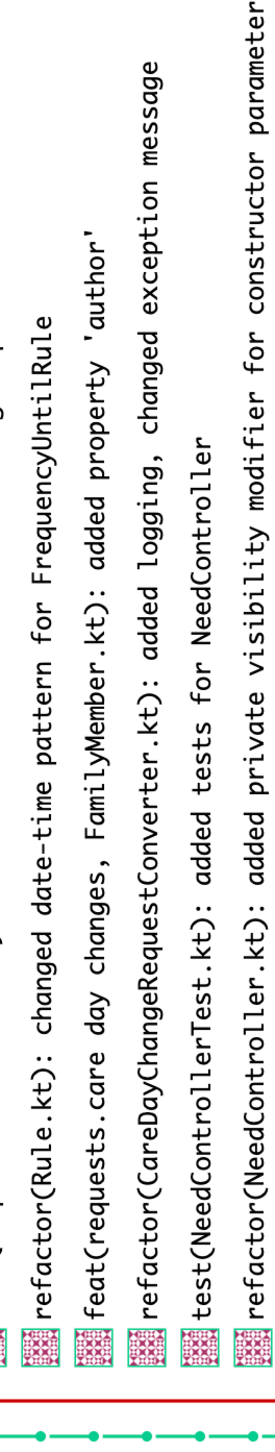
\includegraphics[angle=-90, width=1.0\textwidth]{pdfs/GitLabTree}
	   \caption[Ukázka použití konvence pro práci z~Git]{Ukázka použití konvenci pro práci z~Git na grafu větví}\label{image:gitlab-tree}
    \end{figure}
    Po provedení analýzy pravidel, pravidla byly opraveny podle potřeb tohoto projektu, ale struktura jednotlivé nebyla změněna. Konvence byla zavedena na začátku práce autora na implementaci této bakalářské práce a neměnila se během vývoje. Na obrázku \ref{image:gitlab-tree}) je zobrazen kus grafů větví GitLab po zavedení pravidel. V~následujících podsekcích bude uveden podrobný popis výsledných pravidel po úpravách autora. Struktura pro \verb|commit|, která je definovaná ve zdroji, se skládá ze pěti částí (viz obrázek \ref{code:angular-commit}):
    \begin{itemize}
    \setlength\itemsep{0.3em}
        \item \texttt{typ};
        \item \texttt{rozsah};
        \item \texttt{předmět};
        \item \texttt{tělo};
        \item \texttt{zápatí}.
    \end{itemize}
    
    \subsection{Typ}
        Typ definuje část aplikace, kterou provedený \verb|commit| mění. Seznám hodnot, které je možné zadat, je omezený předem definovaným seznamem:
        \begin{itemize}
        \setlength\itemsep{0.3em}
            \item \texttt{build} -- změny procesu sestavení aplikace nebo úpravy externích závislostí;
            \item \texttt{ci} -- změny týkající se průběžné integrace;
            \item \texttt{docs} -- změny týkající se jenom dokumentace;
            \item \texttt{feta} -- přidání nových funkcí;
            \item \texttt{fix} -- oprava chyb;
            \item \texttt{perf} -- změny zvyšující efektivitu;
            \item \texttt{refactor} -- změny, které nepřidávají nové funkce a současně neopravují chyby;
            \item \texttt{style} -- změny, které nemění význam kódu;
            \item \texttt{test} -- přidaní nebo úprava testů.
        \end{itemize}
    
    \subsection{Rozsah}
        Rozsah definuje konkrétní soubory nebo balíčky, které byly změněny. Uvedený rozsah není povinný, ale v~rámci této bakalářské práce bude rozsah uveden pro každý \verb|commit|. V~případě, že změny byly provedeny současně v~několika různých souborech nebo balíčcích, je potřeba uvést je jako seznam s~položkami v~kulatých závorkách oddělenými čárkami.
    
    \subsection{Předmět}
        Předmět je stručným popisem provedených změn. Změny mají být odděleny od typu dvojtečkou. V~případě, že \verb|commit| obsahuje několik změn, je potřeba je oddělit čárkou. První písmeno každé změny musí být malé. Poslední změna nekončí tečkou.
    
    \subsection{Tělo}
        Tělo je určeno pro podrobnější popis provedených změn. Tato část není povinná, ale je doporučena v~případě, že provedené změny nejsou pochopitelné po přečtení předmětu nebo není jasná příčina provedené změny.
    
    \subsection{Zápatí}
        Zápatí je určeno pro definování přelomových změn a definování závislostí na konkrétní požadavky v~rámci GitHub nebo GitLab\footnote{Webová platforma pro vývoj softwaru pomocí systému řízení verzí Git.}. V~rámci této bakalářské práce jsou každému požadavku v~rámci GitLab přiděleny jednotlivé větve, proto není potřeba uvádět identifikátor požadavku v~zápatí.
    
\section{Použitý jazyk programování}\label{resere:kotlin}
    Současný návrh aplikace byl proveden v~jazyce Kotlin, který je relativně novým jazykem pro JVM\footnote{Java Virtual Machine.}. Poprvé byl tento jazyk představen společností JetBrains v~roku 2011. V~této bakalářské práci byla použita verze 1.3.72 . V~porovnání s~Javou, jejíž podpora je dlouhodobě zaručena společností Oracle, nemá Kotlin předem definovanou periodu podpory, ale podle oficiálních webových stránek zaručuje zpětnou kompatibilitu pro alespoň jednu stabilní verzi, což dovoluje pohodlně migrovat do novější verze jazyka.\cite{java-support-period}\cite{kotlin-compatibility}
    
    %===================================================================
    % Kotlin je relativně nový jazyk pro JVM\footnote{Java Virtual Machine}. Poprvé tento jazyk byl představen společnosti v 2011 roku. První stabilní verze byla představena v únoru roku 2016. Ale už v květnu roku 2017 Kotlin se stal oficiálním jazykem pro Android.
    
    % https://kotlinlang.org/docs/reference/
    Kotlin byl vytvořen jako alternativa k~jazyku Java a řeší některé jeho problémy. Například, Kotlin řeší problém použití \texttt{null}, také známý jako \texttt{The Billion Dollar Mistake}, a problémy s~ním spojené. Java samotna nemá podporu pro \texttt{not-null} proměnné, ale Kotlin takovou podporu má nativně, a to v~podobě oddělení \texttt{nullable} typu pomocí ? operátoru. Pro kompletní seznámení s~jazykem Kotlin je doporučeno navštívit oficiální webové stránky, kde najdeme podrobný návod k~použití jazyka.\cite{kotlin-documentation}
    

\section{Nástroj pro automatizaci sestavování programu}\label{resere:build}
    % https://gradle.org/maven-vs-gradle/
    % https://www.baeldung.com/ant-maven-gradle
    Pro automatizaci sestavování programu se používá nástroj Gradle, který už se používá v~současné implementaci aplikace. Existuje populární alternativa -- Maven, ale Gradle je modernější a pohodlnější. Konfigurace se provádí v~jazyce Groove nebo přímo v~jazyce Kotlin. Také Gradle poskytuje možnost definovat vlastní úkoly spustitelné pomocí příkazové řádky, které pak budou využité pro analýzu a spuštění testů. Podrobnější informaci o~porovnání nástrojů Gradle a Maven lze najít na stránkách \cite{grale-vs-mavem} a \cite{gradle-vs-maven-bealdung}.

\section{Nástroj pro vývoj podnikových aplikací}\label{resere:j2ee}
    % https://spring.io/projects/spring-framework
    % https://spring.io/projects
    % \cite{spring-framework}
    Spring je jeden z~nejznámějších frameworků určených pro vývoj podnikových aplikací. Infrastruktura Spring je velká a komplikovaná. V~době práce na této bakalářské práci se Spring skládal ze 24 aktivních projektů. V~rámci této bakalářské práce bude využito současně několik různých projektů, které zajišťují korektní funkčnost různých aspektů serveru. V~této sekci budou popsány jenom projekty, které budou následně využity při implementaci. Popis je velice stručný a je uveden za účelem pochopení základů použitých technologií. Pro podrobnější informace o~zmíněných projektech je doporučeno navštívit oficiální webovou stránku \cite{spring-projects}.
    
    \subsection{Spring framework}
        Spring framework je základem pro ekosystém různých projektů, které budou popsány v~následujících sekcích.\cite{spring-framework} Tento nástroj samotný je správcem závislostí (\textit{dependency manager}). Spravování závislostí je reprezentováno pomocí principu \texttt{Inversion of Control} (IoC), což znamená, že framework Spring je kontejnerem, který je zodpovědný za vytváření objektů a jejich provázáním mezi sebou. Konfigurace aplikace je reprezentována pomocí rozhraní \texttt{ApplicationContext}.
        
        \begin{figure}
            \begin{minted}{yaml}
spring.profiles.active=dev
            \end{minted}
            \caption{Příklad definování profilu aplikace pomocí proměnné prostředí} 
            \label{code:current-spring-profile}
        \end{figure}
        Pro pohodlnou práci a zvýšení efektivity napsaného kódu má Spring množství dalších užitečných řešení. Jak už bylo zmíněno, popisovat všechno nemá smysl, ale několik nejdůležitějších věcí není možné opomenout. První funkce, která bude široce využita při implementaci, se týká proměnných v~rámci prostředí aplikace. Tyto proměnné umožňují definovat důležité proměnné pro konfiguraci běhu aplikace zvlášť od jejich využití v~kódu. Framework Spring umožňuje využít tyto proměnné přímo v~kódu. Implicitním souborem obsahujícím tyto proměnné je soubor \texttt{application.properties}. Pro zavedení různých proměnných pro různé případy použití aplikace je možné definovat několik takových souborů pro každý z~profilů. Jedinou věcí, kterou je potřeba udělat, je vytvořit soubor, který bude mít v~názvu jméno profilu, kterému patří (\texttt{application-{profile}.properties}). Pro definování, který profil má aplikace použit v~následujících spouštěních, je potřeba v~implicitním souboru zadat potřebný profil jako proměnnou (viz obrázek \ref{code:current-spring-profile}). 
        
        
        \begin{figure}
            \begin{minted}{Kotlin}
@Bean
@ConditionalOnProperty(
        value = ["scheduled.alimonyFactory"],
        matchIfMissing = false,
        havingValue = "true")
fun startAlimonyFactory(): AlimonyFactory {
    logger.info("Schedule job: starting AlimonyFactory")
    return AlimonyFactory(
            alimonySettingRepository,
            alimonyRepository)
}
            \end{minted}
            \caption{Příklad aspektově orientovaného programování v~Spring} 
            \label{code:spring-conditional}
        \end{figure}
        Spring framework používá techniku vkládání závislosti (\textit{dependency injection}), což dává možnost psaní kvalitnějšího softwaru, ale Spring poskytuje možnost zlepšit výsledný kód ještě více. Framework Spring také používá paradigma aspektově orientovaného programování (AOP). Toto paradigma má za cíl zvýšit modularitu výsledného softwaru pomocí rozdělení kódu do logických částí, nalezení opakujících se částí, které jsou také nazývané průřezové problémy, a nahrazení opakujícího se kódu. Příkladem AOP je anotace zaměřená na podmíněné spouštění metody v~závislosti na výsledku předem definované podmínce v~závorkách (viz obrázek \ref{code:spring-conditional}).
    
    \subsection{Spring Boot}
        % https://docs.spring.io/spring-boot/docs/current/reference/html/spring-boot-features.html#boot-features-external-config
        Spring Boot je pomocný nástroj pro programátora při konfiguraci aplikace využívající framework Spring. Spring Boot registruje 17 různých implicitních zdrojů proměnných. Kompletní popis zdrojů je na oficiálních stránkách dokumentace \cite{spring-property-sources}. Podle nalezených proměnných framework provádí analýzu konfigurace aplikace a následně, pomocí anotací pro podmínky, automaticky nastavuje prostředí aplikace. Navíc od klasického frameworku Spring, Sping Boot obsahuje rozšířený seznam anotací pro podmínky, které jsou široce využity pro zmíněnou automatickou konfiguraci.\cite{spring-boot}
    
    \subsection{Spring Security}
        Spring Security je framework určený pro návrh autentizace, autorizace a filtrů. Framework vyžaduje využití frameworku Spring, případně i frameworku Spring Boot. Podrobné informace lze najít na oficiálních stránkách \cite{spring-security}.
    
    \subsection{Spring Data}
        % https://docs.spring.io/spring-data/jpa/docs/current/reference/html/#repositories.query-methods
        Spring Data je framework pro pohodlnou práci programátora při implementaci datové vrstvy\footnote{Vrstva aplikace, která komunikuje s~databází.}. Framewok vytváří dodatečnou vrstvu nad implementací Java Persistense API\footnote{Application programming interface.} (JPA). Implementací JPA může být EclipseLink nebo Hibernate. Příkladem využití je rozhraní \texttt{CrudRepository}, které bude využito v~této bakalářské práci. Rozhraní definuje základní operace s~databází a dovoluje programátorovi jenom definovat typ entity a typ primárního klíče. V~případě, že programátor potřebuje složitější dotazy na databázi, framework poskytuje možnost definování metod, které ve svých názvech obsahují popis dotazů~\cite{query-methods}. Framework rozebírá název na jednotlivé části a překládá ho na SQL\footnote{Structured Query Language.} dotaz.
    
    \subsection{Spring Web Services}
        Spring Web Services je framework určený pro implementaci webových služeb. V~rámci této bakalářské práce bude tento framework využit pro implementaci aplikační vrstvy serveru. Aplikační vrstva aplikace má pokrývat případy užití aplikace. Podrobnou informaci lze najít na oficiálních stránkách~\cite{spring-web-services}.
        

%  \section{Spring Boot}\label{reserse:spring-boot}
    % https://spring.io/projects/spring-boot
    % \cite{spring-boot}
    % TODO Spring Boot je nástrojem určeným pro rychlý a
    
\section{Testování}\label{reserse:testovani}
    Testování aplikace se skládá z~několika částí. První část je testování softwaru samotného pro ověření jestli jednotlivé metody, třídy nebo celé moduly fungují správně a komunikují mezi sebou bezchybně. Druhou částí testování je ověření, jestli testy pokrývají dostatečnou část kódu a jestli pokrývají důležité funkce. V~této sekci jsou popsány nástroje pro zaručení kvalitního testování, které budou následně využity při implementaci testů a jejich analýze.
    
    \subsection{Spring}
        Framework Spring poskytuje velký počet nástrojů pro testování softwaru. Každý z~dodatečných frameworků, jako Spring Boot nebo Spring Security, spolu s~novými funkcemi, přidávají vhodné nástroje pro kvalitní testování těchto funkcí. Celý přehled nástrojů, které poskytuje framework, je na oficiálních stránkách dokumentace~\cite{spring-tests-doc}. V~této sekci jsou uvedeny jenom nejdůležitější použité nástroje.
        
        Prvním nástrojem je anotace \texttt{SpringBootTest}, kterou poskytuje framework Spring Boot pro implementaci integračních testů. Při použití této anotace framework vytvoří nutný kontext aplikace pro kompletní testování.
        
        Druhým důležitým nástrojem je třída \texttt{MockMvc}, která poskytuje možnost kvalitního testování aplikační vrstvy serveru. Tento nástroj je součástí frameworku Spring Web Services.
        
    \subsection{JUnit}
        JUnit je framework určený pro testování softwaru. V~této bakalářské práci bude použita verze 5. Tento framework bude použit pro vytvoření kostry testování. Podrobnější informace o~funkcích frameworku je dostupná na oficiálních webových stránkách~\cite{junit-doc}.
        
    \subsection{JaCoCo}\label{resere:testovani:jacoco}
         %https://www.jacoco.org/jacoco/trunk/doc/implementation.html
        JaCoCo je nástroj poskytující podrobnou analýzu testů. Tento nástroj bude použit pro výslednou analýzu implementovaných testů a také jako pomocný nástroj pro nalezení důležitých neotestovaných funkcí během implementace testů. Nástroj existuje v~reprezentaci přídavného modulu pro nástroj Gradle, který se již používá v~současné implementace programu. Výsledky práce jsou následně uloženy do předem definované složky a jsou reprezentovány pomocí HTML\footnote{Hypertext Markup Language.} stránek. Nástroj je otevřeným softwarem, proto podrobnou informaci o~implementaci lze najít na oficiálních stránkách~\cite{jacoco-implementation}. Výsledky analýzy podle JaCoCo jsou dostupné v~příloze \ref{dodatek:code-coverage}.
        
    \subsection{IntelliJ IDEA}\label{resere:testovani:intellij-idea}
        % https://www.jetbrains.com/help/idea/code-coverage.html
        % TODO nastroj pro analyzu pokryti kodu testy \cite{intellij-idea-code-coverage}
        Pro provedení analýzy testů také bylo využito vývojové prostředí IntelliJ IDEA, používané autorem této práce pro implementaci programu. Nástroj pro pokrytí kódu testy je implicitním nástrojem zmíněného vývojového prostředí a poskytuje možnost zobrazování výsledků analýzy přímo v~kódu. Takový přístup zrychluje proces implementace testů. Nástroj také dovoluje vygenerovat výsledky zvlášť od kódu, proto tyto výsledky jsou také dostupné v~příloze \ref{dodatek:code-coverage}.


\section{Dokumentace}\label{resere:dokumentace}
    Pro dokumentace API v~současné implementaci aplikace se používá framework Swagger. Důležitou funkcí, kterou framework poskytuje, je automatické generování dokumentace na základě přidaných anotací v~kódu. Dokumentace je následně dostupná z~internetu ze stejné adresy jako server, ale na jiném portu. Podrobná informace o~framewoku je dostupná na oficiálních webových stránkách~\cite{swagger-doc}.
    
\section{Použité databáze}\label{resere:databaze}

    \subsection{H2}
        % Pro proces vývoje a testování byla zvolena databáze H2\cite{h2-db}, která je relační databází. 
        % http://www.h2database.com/html/tutorial.html
        Současná implementace používá relační databáze H2. Hlavním důvodem zvolení právě této databáze je možnost volby několika různých režimů, kde jeden z~režimu je vestavěný režim. Tento režim usnadňuje programátorovi práci s~databází, protože se databáze vytváří při spuštění programů a zaniká při jejich zastavení. Soubory s~daty jsou uloženy na disku nebo přímo v~paměti. H2 má též vlastního manažera, který je dostupný přes webový prohlížeč. Podrobnější informace jsou dostupné na oficiálních webových stránkách~\cite{h2-doc}.
        
    \subsection{PostgreSQL}
        % https://www.postgresql.org/docs/12/index.html
        % https://docs.spring.io/spring-cloud-dataflow/docs/1.1.0.RELEASE/reference/html/configuration-rdbms.html
        PostgreSQL je široce využívanou objektově relační databází napsanou v~jazyce C. V~době odevzdání této bakalářské práce je databáze PostgreSQL udržována skupinou Global Development Group a je otevřeným softwarem. Pro implementaci byla zvolena poslední stabilní verze -- 12. Kompletní dokumentace je dostupná online~\cite{postgres-documentation}. Framework Spring, zmíněný v~sekci \ref{resere:j2ee}, nativně podporuje použití PostgreSQL.
        

\section{Nástroj pro analýzu rozsahu implementace}\label{reserse:cloc}
    Nástroj CLOC\footnote{Count Lines of Code.}\cite{cloc-download} poskytuje možnost spočítat počet řádek kódu je v~dané složce. Nástroj podporuje velký počet programovacích jazyků programování. Výsledek obsahuje počet řádek kódu oddělený od komentářů a prázdných řádek. Tento nástroj bude použit pro analýzu současné implementace aplikace a analýzu provedené práce v~rámci bakalářské práce.

\chapter{Analýza}
\label{chapter:analyza}
Hlavním cílem teto bakalářské práce je implementovat návrh backendu podle návrhu a fragmentu implementace, které byly udělány v rámci předmětů BI-SP1 a BI-SP2 bakalářského studia vyučovaných na FIT ČVUT v akademickém roce 2018/2019 a 2019/2020. Tato kapitola se zabývá analýzou výsledků zmíněných předmětu. Autor práce je zároveň i absolventem těchto předmětů, kde pracoval v týmu na analýze požadavku zákazníka a pak pracoval jako backend vývojář a vedoucí backendového týmu.

Pro jasné zajištěni verze aplikace, která bude předmětem analýzy teto kapitoly, uvádím datům ukončení práce na projektu v rámci předmětu BI-SP2 - 25. února 2020. Také pro možnost pohodlně vyhledat konkretní verze uvádím poslední 
\textit{commit}\footnote{252b0288dbfe9942446b78fd452c0edce810a370} udělaný v rámci tohoto předmětu.

% Tato kapitola se zabývá popisem současného stavu aplikace, který je výsledkem zmíněných předmětů.

% Hlavním cílem teto bakalářské práce je implementovat návrh backendu podle návrhu a fragmentu implementace, které byly rozpracovány v rámci předmětů BI-SP1 BI-SP2 bakalářského studia vyučovaných na FIT ČVUT. Dalším cílem teto práci je navrhnou vhodné úpravy za účelem dosažení kvalitnějšího výsledku a splnění požadavku frontedové častí aplikace. Autor teto práci absolvoval zmíněné předměty, proto pro zajištění rozdilu v 

\section{Analýza současného návrhu} \label{analyza:analyza navrhu}
    
    \subsection{Předmět BI-SP1}\label{analyza:navrh:sp1}
    V rámci předměty BI-SP1 pracovalo sedm lidí včetně autora teto práci. Tým měl za úkol analýz požadavku zákazníka a návrh implementaci aplikace. Aplikace se skládá ze dvou částí. Serverového backendu, který je předmětem teto bakalářské práci a frontendové častí aplikace, kterou současně v rámci bakalářské prací implementuje kolega - Martin Beran. Frontendová část aplikace je Android aplikací. Backendová část je serverovým backendém, který má poskytovat REST\footnote{Representational State Transfer} API pro Android aplikaci.
    
    Během semestru tým provedl kompletní analýzu požadavku zákazníka. Především, tým navrhl scénáře použiti aplikace:
    \begin{itemize}
	   \item Přihlašování/Registrace;
	   \item Přihlašování/Registrace do rodiny;
	   \item Role v aplikace a jejich vytváření;
	   \item Nastavení pečovatelský dnů;
	   \item Kalendář;
	   \item Kniha potřeb dítěte;
	   \item Uchování účtenek;
	   \item Správa alimentů.
	\end{itemize}
    Potom byly navrženy Use Case Diagram a Activity Diagramy, podle kterých byly navrženy Wireframy a Doménový model. 
    
    \subsection{Předmět BI-SP2}\label{analyza:navrh:sp2}
        Cílem předmětu BI-SP2 byla implementace návrhu předmětu BI-SP2. Autor teto práce pracoval v backendovém týmu a zároveň vystupoval v roli vedoucího backendového týmu.
        
        Pro vývoj backendové častí aplikace byl zvolen jazyk Kotlin, zmíněný v sekci \ref{resere:kotlin}, a framework Spring, zmíněný v sekci \ref{resere:j2ee}. Jako {buildovací system}\footnote{nástroj pro automatizaci sestavování programu} byl zvoleny nástroj Gradle. Podrobnnějí výsledky předmětu BI-SP2 probrány v sekce \ref{analyza:soucasnaImplementace}.
        
    
    \subsection{Doménový model}\label{analyza:navrh:DomainModel}
        Hlavním zdrojem informace o výsledném návrhu serveru je Doménový model. Kompletní Doménový model se nachází v příloze \ref{dodatek:DomainModel}. Zelenou barvou jsou označeny třídy, které už jsou implementovány. žlutou barvou jsou označeny třídy, které ještě nejsou implementovány. Také, jsou třídy označeny zároveň žlutou a zelenou barvou, což znamená, že třída je implementována jenom částečně. Taková situace se mohla nastat v případe, že implementace vyžadovala implementace jiné třídy, která ještě neexistovala. Tento Doménový model má určité nedostatky podle požadavku frontedové části aplikace. Jako příklad takových nedostatku je možné uvést zbytečně komplikovaný návrh Intervalů (viz. obrázek \ref{image:Interval1}), který byl od začátku předělán.

    \subsection{Registrace a přihlášeni do rodiny}
        Aplikace je navržena tak, že první uživatel, který má vytvořit svůj účet je jeden z rodičů. Pro registraci člověk potřebuje řadu povinných údajů:
        \begin{itemize}
	        \item \textit{name} - zvolené jméno se stává jeho implicitním jménem v systému
	        \item \textit{surname} - zvolené příjmení se stává jeho implicitním příjmením v systému
	        \item \textit{email} - zvolený email je identifikátorem uživatele v rámci systému
	        \item \textit{password} - heslo pro autorizaci v systému
        \end{itemize}
        Na základe těchto údajů se vytváří unikátní uživatel v rámci systému. V tomto stavu člověk není přihlášeny do žádné rodiny a nemá žádnou roli. Podrobněji role budou popsané v sekci \ref{analyza:bezpecnost:role}. \textit{User} také může mít implicitní obrázek profilu (viz. obrázek \ref{image:User-Image1}).
        \begin{figure}\centering
	        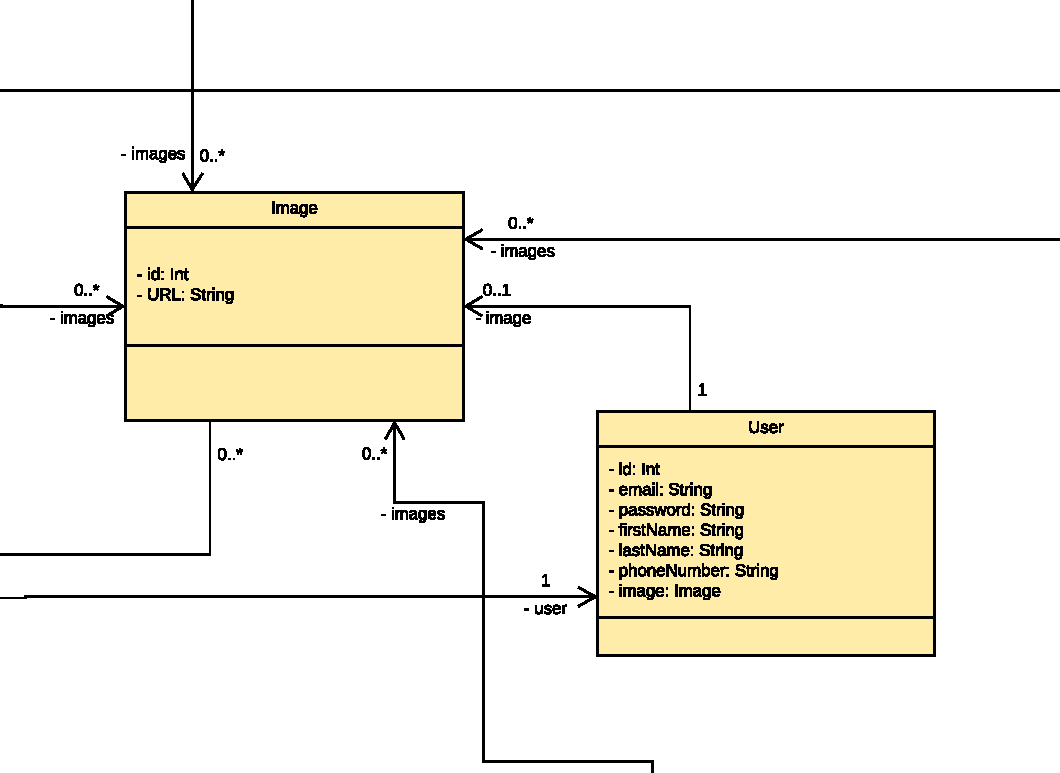
\includegraphics[width=0.5\textwidth]{pdfs/User-Image1}
	        \caption[Návrh User-Image]{Vztah mezi třídami \textit{User} a \textit{Image} podle Doménovém modelu z předmětu BI-SP2}\label{image:User-Image1}
        \end{figure}
        
        Potom uživatel má možnost vytvořit rodinu nebo přihlásit se do již existující rodiny. Pro vytvoření nové rodiny, uživatel potřebuje zadat jméno rodiny a přidat členy rodiny. Autor teto rodiny automaticky se stává jedním s rodičů teto rodiny. jinou možností je přihlásit se do rodiny, která již existuje. Podmínkou k tomu je existování pozvání do některé existující rodiny. V takovém případě uživatel už nemá možnost zvolit role v rámci rodiny. Role má být nastavena uživatelem, který vytvořil toto pozvání.

    \subsection{Kalendář}    
        Kalendář je hlavním zdrojem informaci pro celou rodinu, který společný pro všechny uživatele. Na něm jsou zobrazené zvýrazněné různými barvami pečovatelské dny obou rodičů a důležité události, které mohou být jednorázové nebo pravidelné. 
        
        Kromě dlouhodobých nastavení pečovatelských dnu, kalendář může zobrazovat i jednorázové změny, které mohou vidět všechny členy rodiny. Takový postup pomáhá rodině eliminovat situace, kdy několik členu rodiny najednou myslí, že je v konkretní den dítě v jejích péči nebo několik členu rodiny najednou říkají, že není to jejích den.  
    \subsection{Alimenty}    
        Aplikace řeší i finanční problémy. Hlavní problémem jsou alimenty, které má pravidelně uhrazovat jeden z rodičů. Tento proces byl rozdělen do dvou častí. První častí je nastavení dlouhodobých pravidel (viz. obrázek \ref{image:AlimonySettings1}) pro splacení alimentů. Druhou častí jsou samotné alimenty (viz. obrázek \ref{image:Alimony1}), které se generuje na základě dlouhodobých nastavení. Jedna rodina může mít zároveň několik nastavení v případě, že jedna rodina má několik dětí nebo chce rozdělit alimenty do logický částí.
        \begin{figure}\centering
	        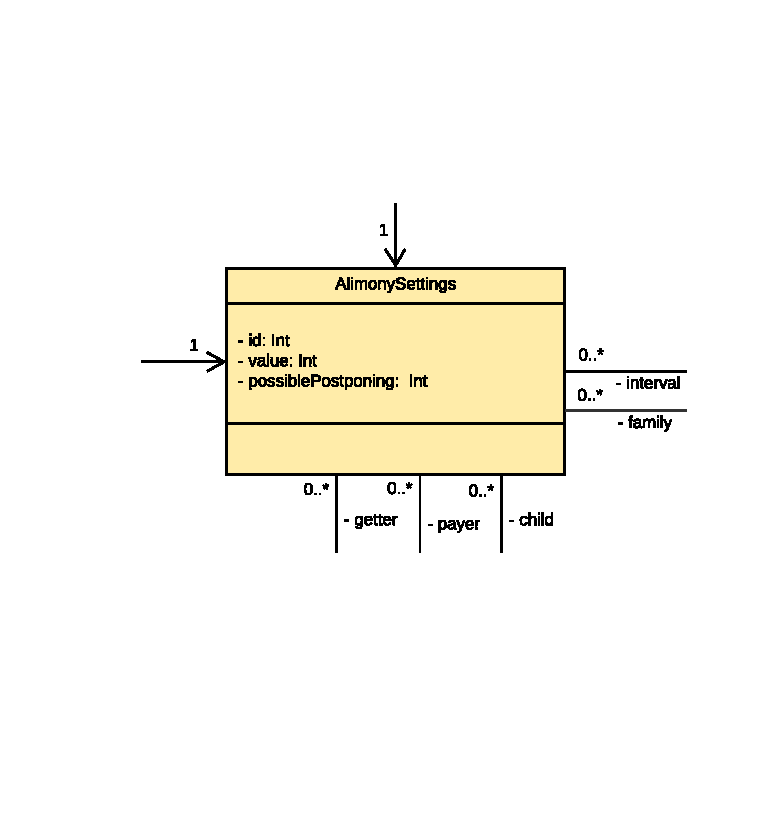
\includegraphics[width=0.5\textwidth]{pdfs/AlimonySettings1}
	        \caption[Návrh AlimonySettings]{Návrh třídy \textit{AlimonySettings} podle Doménovém modelu z předmětu BI-SP2}\label{image:AlimonySettings1}
        \end{figure}
        \begin{figure}\centering
	        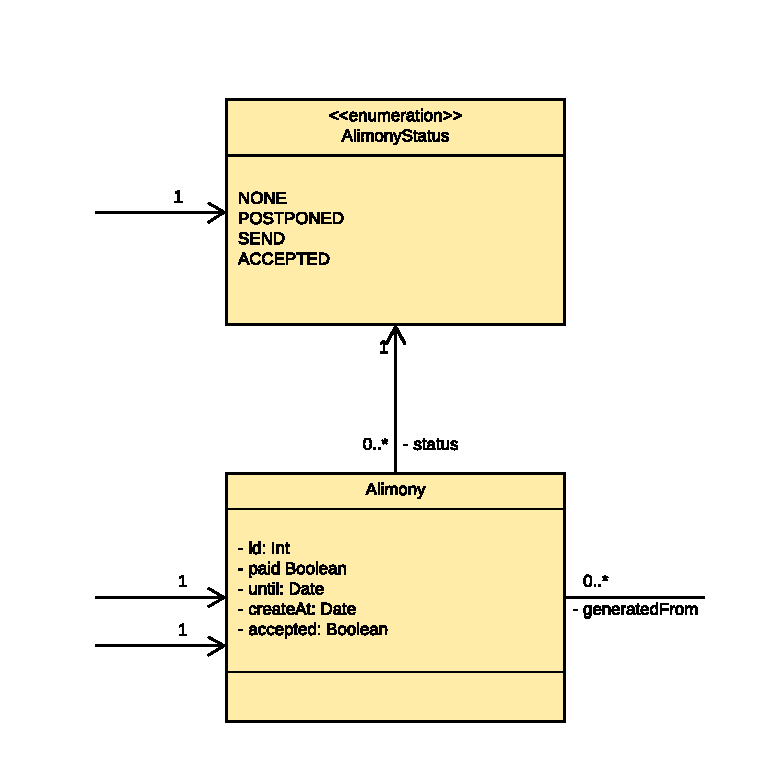
\includegraphics[width=0.5\textwidth]{pdfs/Alimony1}
	        \caption[Návrh Alimony]{Návrh třídy \textit{Alimony} podle Doménovém modelu z předmětu BI-SP2}\label{image:Alimony1}
        \end{figure}
    \subsection{Kniha potřeb dítěte}
    
        Jedním s populárních problému, který vzniká v procesu rozvodu, je nakupování příliš drahých věci o kterých nevědí ostatní členy rodiny. Jako příklad je možné uvést nakupování bot pro dítěte. Jeden s rodičů může chtít "koupit lásku dítěte" a koupit několikrát dražší boty než dítěte opravdu potřebuje. Kniha potřeb dítěte (viz. obrázek \ref{image:Need1}) je zaměřena na překonání takových situací.
        \begin{figure}\centering
	        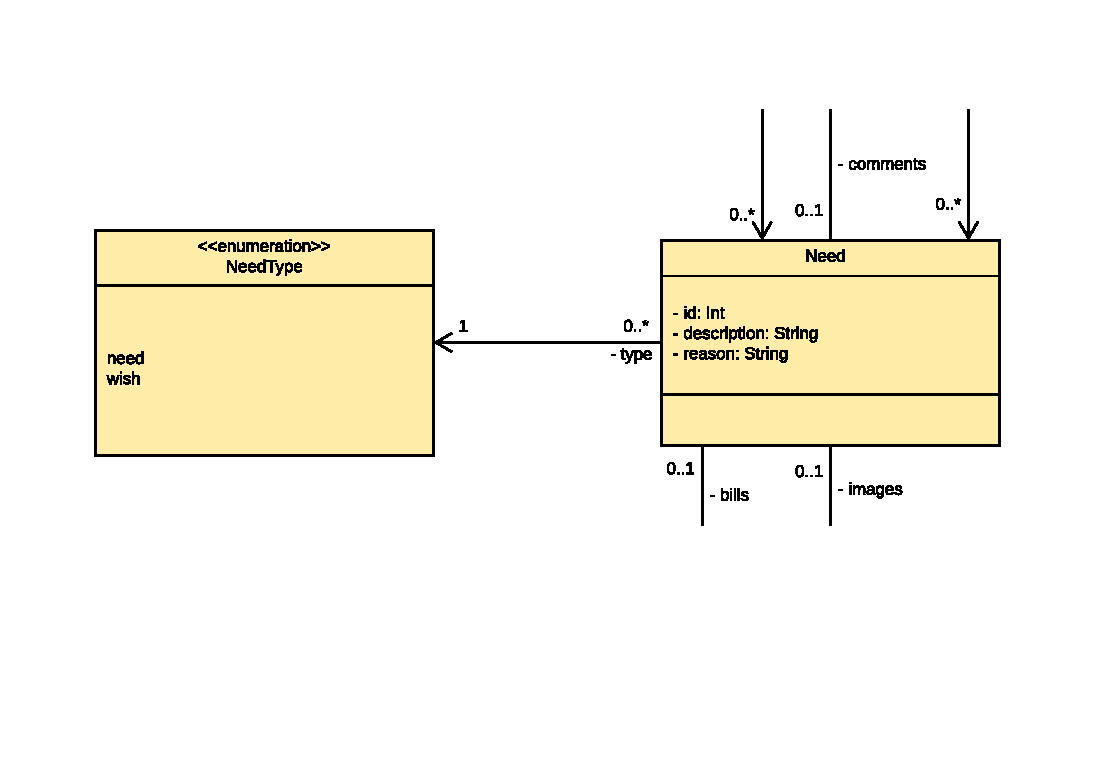
\includegraphics[width=0.5\textwidth]{pdfs/Need1}
	        \caption[Návrh Need]{Návrh třídy \textit{Need} podle Doménovém modelu z předmětu BI-SP2}\label{image:Need1}
        \end{figure}
        
        Potřeba může být typu \textit{need} a \textit{wish}. Podle současného návrhu je rozdíl mezi typy pouze pro informační účely. Každé instance \textit{Need} patři instance \textit{NeedPermission} (viz. obrázek \ref{image:NeedPermissions1}), která definuje přístupová práva pro jednotlivého člena rodiny. V případě, že uživatel nemá žádné z přístupových práv, pak tento záznam nemá ve svém seznamu potřeb dítěte. Toto pravidlo se netýká jenom rodíču, která mají pŕístup ke všemu. 
        \begin{figure}\centering
	        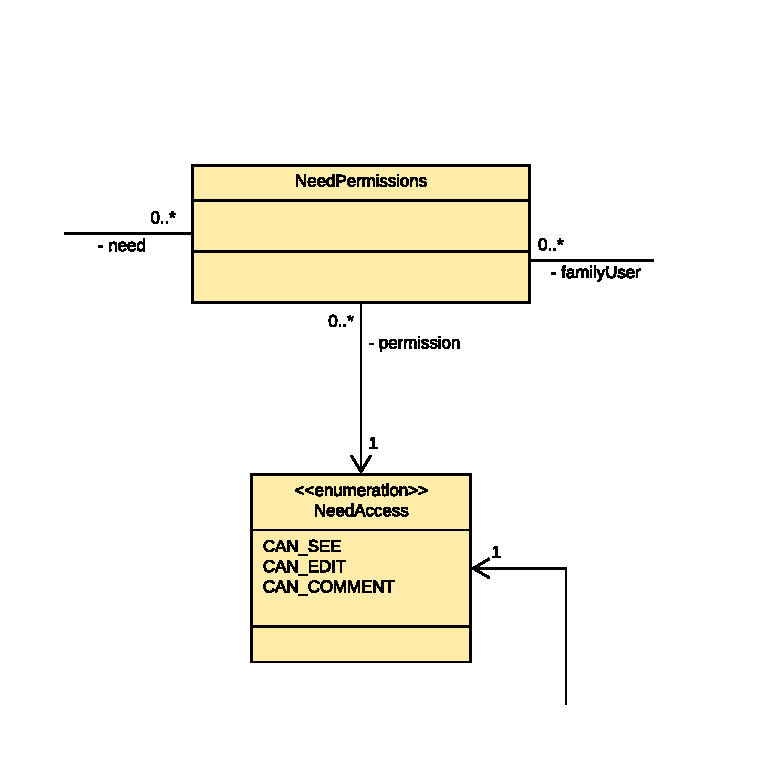
\includegraphics[width=0.5\textwidth]{pdfs/NeedPermissions1}
	        \caption[Návrh NeedPermissions]{Návrh třídy \textit{NeedPermissions} podle Doménovém modelu z předmětu BI-SP2}\label{image:NeedPermissions1}
        \end{figure}
       
       Potřeba má v sobě následující informace:
        \begin{itemize}
            \item \textit{description} - popis potřeby
            \item \textit{reason} - příčina proč dítě tohle potřebuje
            \item \textit{images} - obrázky věcí, kterou dítě potřebuje
            \item \textit{bills} - účtenky v případě, že někdo z rodičů splnil potřebu
            \item \textit{comments} - komentáře členu rodiny včetně dítěte
        \end{itemize}
     
\section{Analýza současné implementace}\label{analyza:soucasnaImplementace}
    Projekt má ve složce \textit{main}\footnote{bi-springboot/src/main} 69 souborů a 845 řádek kódů. Implementace částečné pokrývá Doménový model zmíněný v sekci. \ref{analyza:navrh:DomainModel}.
        
    \subsection{Implementované třídy}
        Seznam implementovaných entit:
        \begin{itemize}
            \item \textit{AlimonyStatus}
            \item \textit{Bill}
            \item \textit{CalendarEvent}
            \item \textit{OneTimeEvent}
            \item \textit{Comment}
            \item \textit{FamilyMember} - částečně
            \item \textit{History}
            \item \textit{IntervalType}
            \item \textit{NWeekInterval}
            \item \textit{WeekInterval}
            \item \textit{NeedAccess}
            \item \textit{NeedType}
            \item \textit{NeedType}
            \item \textit{AbstractPermissions}
            \item \textit{Permissions}
            \item \textit{RequestStatus}
            \item \textit{User}
        \end{itemize}
        
        Byl přidány \textit{Controller} pro testování, zda aplikace běží. \textit{Controller} je namapován na \textquote{/}. Také, byl přidaná třída, která obsahuje nápovědy pro ostatní \textit{Controllery} ohledně zachycování chyb. Tato třída byla zavedena za účelem poskytování uživateli jenom korektně formátovanou informaci  a filtrování zbytečné informace pro koncového uživatele (viz. tabulka \ref{tab:excpetion-handler1}). 
        \begin{table}\centering
	    \caption[Exception handler]{Ukázka \textit{Exception handler} podle návrhu BI-SP2}\label{tab:excpetion-handler1}
	    \begin{tabular}{|l|c|c|c|}\hline
		  Typ chyby		& HTTP status		& zprava	& URL	\tabularnewline \hline \hline
		  \textit{IllegalAccessException}	& 401	& původní zprava chyby		& původní cesta     \tabularnewline \hline
		  \textit{IllegalArgumentException}	& 400	& původní zprava chyby		& původní cesta     \tabularnewline \hline
		  \textit{NullPointerException}	& 500	& původní zprava chyby		& původní cesta     \tabularnewline \hline
		  \textit{NoSuchElementException}	& 404	& nic		& nic     \tabularnewline \hline
	    \end{tabular}
        \end{table}
    
    \subsection{Dokumentáce API}
        Bylo provedeno nastavení frameworku Swagger\ref{resere:dokumentace} pro dokumentace API (viz. obrázek \ref{code:swagger-configuration}). Podrobněji framework Swagger byl popsán v sekci \ref{resere:dokumentace}.
        \begin{figure}
        \begin{minted}{java}
@Configuration
@EnableSwagger2
class SwaggerConfig {
@Bean
fun api(): Docket {
    return Docket(DocumentationType.SWAGGER_2)
        .select()
        .apis(RequestHandlerSelectors.any())
        .paths(PathSelectors.any())
        .build()
    }
}
        \end{minted}
        \caption{Ukázka nastavení frameworku Swagger}\label{code:swagger-configuration}
        \end{figure}
    
    \subsection{Profily}
    %spring profiles: https://docs.spring.io/spring-boot/docs/current/reference/html/spring-boot-features.html#boot-features-profiles
    %applicatioon peoperties: https://docs.spring.io/spring-boot/docs/current/reference/html/spring-boot-features.html#boot-features-external-config-application-property-files
        Framework Spring poskytuje možnost rozdělit implementaci do logických bloků, které budou existovat jenom v konkrétních profilech\cite{spring-profile}. Implicitně všechny komponenty nezávisle na aktuálních profilech. Pro zavedení profilů pro konkretní komponentu je potřeba ji označit anotací \textit{Profile}. V závorkách vedle anotací je potřeba přidat seznam profilu, ve kterých tato komponenta bude existovat. Konfigurace aktuálně zapnutých profilů se provádí pomocí souboru \textit{application.properties}\footnote{TODO}, který definuje \textit{property}\footnote{TODO} pro prostředí aplikace.
    
        Každý profil také může obsahovat vlastní konfigurační soubor, který definuje všechny nutné \textit{property}. Soubor má byt zadán ve formátu \textit{application-\{profile\}.properties}, kde \textit{profile} je názvem profilu kterému patří tento soubor. Současný návrh aplikace obsahuje dva konfiguračních souboru.
    
        První konfigurační soubor obsahuje implicitní \textit{property} pro prostředí aplikace. Aktuálně soubor má jenom definici aktuálního profilu aplikace. 
    
        Druhý konfigurační soubor patří profilu \textit{development}. Tento profil je určen pro pohodlný proces vývoje aplikace. Soubor obsahuje konfiguraci databáze a konfiguraci žurnálu aplikace. Podrobněji použita databáze pude popsána v sekci \ref{analyza:soucasnaImplementace:databaze}.
    \subsection{Databáze}\label{analyza:soucasnaImplementace:databaze}
        Pro proce vývoje byla zvolena relační\footnote{relacni DB TODO} databáze H2\cite{ht-db}. Zvolená databáze umožňuje vytvářet tabulky při každém zapuštěni aplikace přímo v pamětí aplikace. Podrobněji tato databáze a její princip fungování byly popsány v sekci \ref{resere:databaze}
    
\section{Analýza požadavku frontendu}\label{analyza:pozadavky-frontendu}
    V rámci předmětu BI-SP2 současně s implementací backendové častí aplikace, probíhala implementace forntendové častí aplikace - Android aplikace. Během vývoje frotnendové častí aplikace byly zjištěny nedostatky, které zbytečně komplikují implementaci, jak backendu, tak i frontendu.
    \subsection{Interval}
        Prvním takovým příkladem je návrh intervalu\ref{image:Interval1}, které jsou široce využívány v projektu. Návrh řešení tohoto problému bude popsán v sekci \ref{navrh:upravy}. tady bude popsán jenom problém samotný. Entita \textit{Interval} reprezentuje časové rozmezí pro pečovatelské dny, opakované události, nastavení alimentů a navazující na ně požadavky na změny a historické záznamy.
            
        Jádro problému je v tom, že entita je navržena pomoci generalizace, neboli dědičnosti z hlediska implementace. Takový návrh dává možnost vytvořit konkretní typ intervalu pomocí zvolení odpovídající třídy, ale na druhou stranu působí komplikace při implementace a nepokrývá všechny možné případy potřebných intervalu. Například, není možné sestavit interval, který se bude opakovat každý poslední den měsíce. Pokud by jsme chtěli se držet se aktuální implementaci a zároveň pokryt všechny možné případy, ztratili bychom přehlednost zvolení správné třídy při vytváření instance \textit{Intervalu}.
            
        Dalším problémem \textit{Intervalu} je provázanost s pečovatelskými dny. Podle návrhu frontendové častí se bylo zjištěno, že pečovatelské dny nepotřebují komplikované nastavení a zároveň bych potřebovali mít odkazy na konkretního rodiče, který je zodpovědný za dítěte v tento den nebo časový úsek.
    
    \subsection{Alimenty}
        Druhou úpravou návrhu backendu, kterou potřebuje frontend, se tyká entity \textit{ALimony}.
        Tato entita reprezentuje alimenty, které jeden rodič má posílat druhému rodiče. Jedna instance se odpovídá alimentům za jeden měsíc. Současný návrh popisuje návrh entity a její navázanost na entitu \textit{AlimonySettings}(viz. obrázek \ref{image:aliomny-draft1}), která definuje dlouhodobou konfiguraci, na základě které se vytváří jednotlivé instance alimentů. Nastavení alimentů se platí v rámci jedné rodiny. V případě potřeby, rodiče mají možnost rozdělit alimenty do několika nastavění. 
        
        Hlavní problém je v tom, že instance alimentů by se měly vytvářet nezávisle na frontendové části aplikace. Podrobně návrh řešení problému bude popsán v sekci \ref{navrh:upravy:alimenty}.
        
        Dodatečným požadavkem frontendového týmu se týká entity \textit{Alimony} samotné. Za účelem zjednoduďení návrhu frontendové části je potřeba přidat závislost na entitu \textit{Family}. % V takovém pŕípade aplikace může ihned po nalazení novych alimentu rict uZivateli ktere rodine patri tyto alimenty.
        \begin{figure}\centering
	        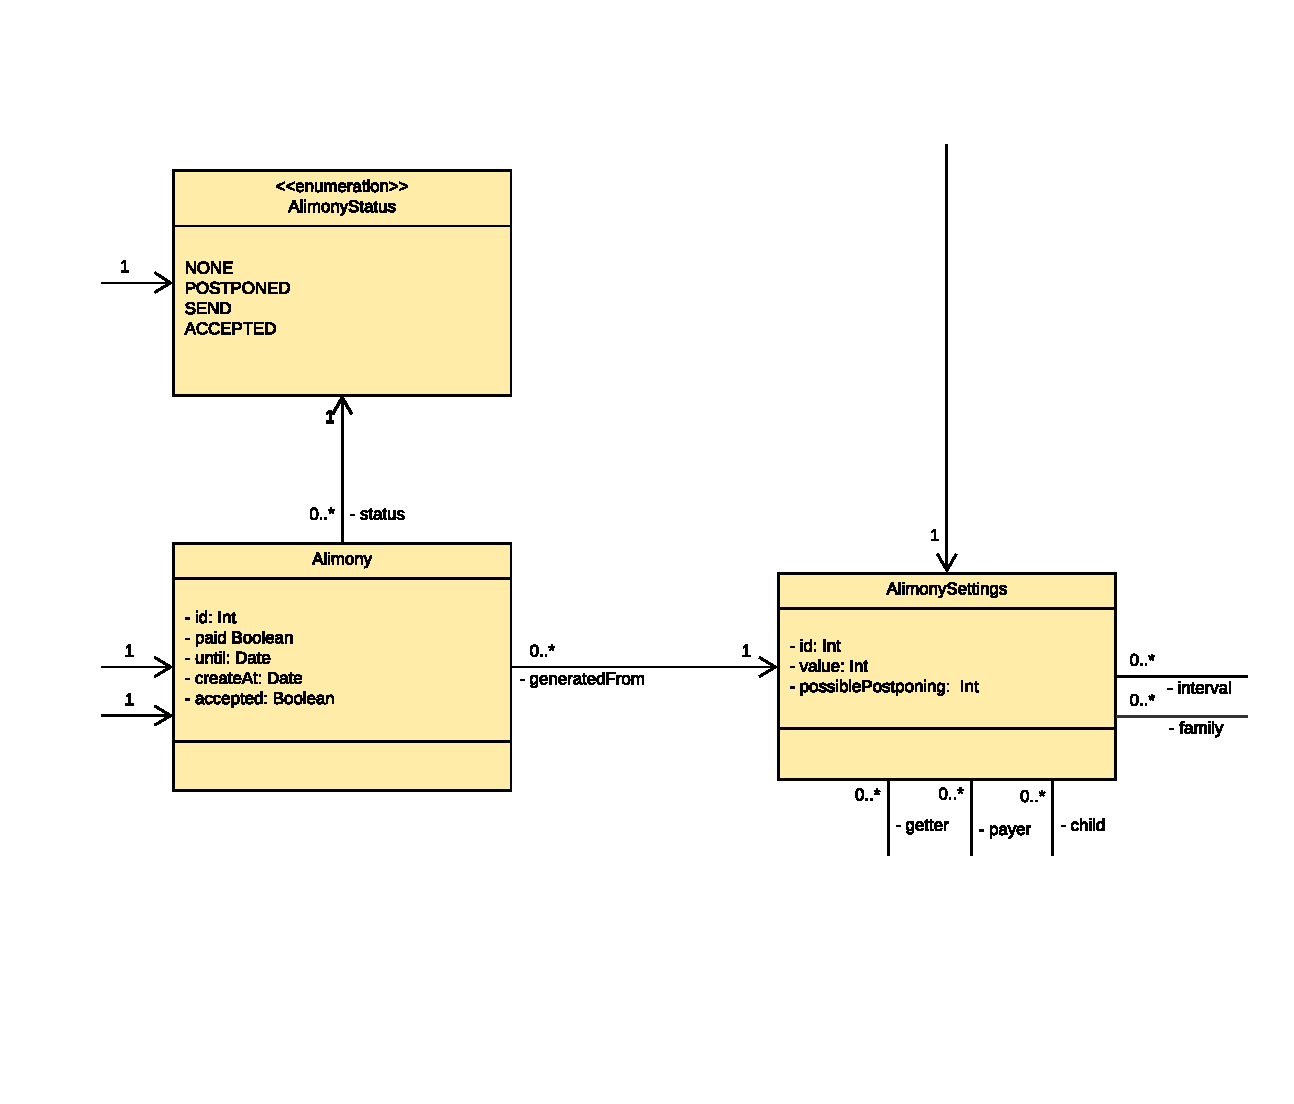
\includegraphics[width=0.5\textwidth]{pdfs/AlimonyDraft1}
	        \caption[Návrh \textit{Alimony} a \textit{AlimonySettings}]{Návrh entit \textit{Alimony} a \textit{AlimonySettings} podle Doménovém modelu z předmětu BI-SP2}\label{image:aliomny-draft1}
        \end{figure}
    % \section{Analýza konkurence}
    %     Tento návrh...
% \section{Analýza testování}

\section{Analýza bezpečnosti}
    
    \subsection{Role}\label{analyza:bezpecnost:role}
    
    % Aplikace je navržená tak, že první věc, kterou uživatel udělat, je registrace. Uživatel potřebuje zvolit jméno, příjmení, email a heslo. Na základě těchto údajů se vytváří účet uživatele. V Doménovém modelu tato třída se jmenuje \textit{User}. V tento okamžik uživatel má role \textit{USER}, která mu nadává možnost udělat jenom omezený počet věcí.  
        Než se uživatel přihlásí do rodiny, nemá žádnou roli nebo má roli uživatele bez rodiny. V takovém stavu uživatel by měl mít velice omezena přístupová práva. 
        
        Po přihlášeni do rodiny uživatel má svou vlastní roli (viz. obrázek \ref{image:Role1}), podle které mohou lišit jeho přístupová práva. Hlavní rolí v aplikace je rodič. Uživatel s takovou rolí má přístup ke všem potřebám dítěte a všem záznamem v kalendáři. Také, rodič může vytvořit pozvání do rodiny pro libovolného uživatele a nastavit mu libovolnou roli, včetně roli rodiče. Mimořádnou roli v rámci systému je dítěte. Uživatel s takovou rolí nemůže vlastnit pečovatelský den nebo splnit přání. Přihlášení dítěte muže proběhnout i bez vytvořeni klasického uživatele systému. Ostatní uživatele v rodině mají roli příbuzného.
        \begin{figure}\centering
	        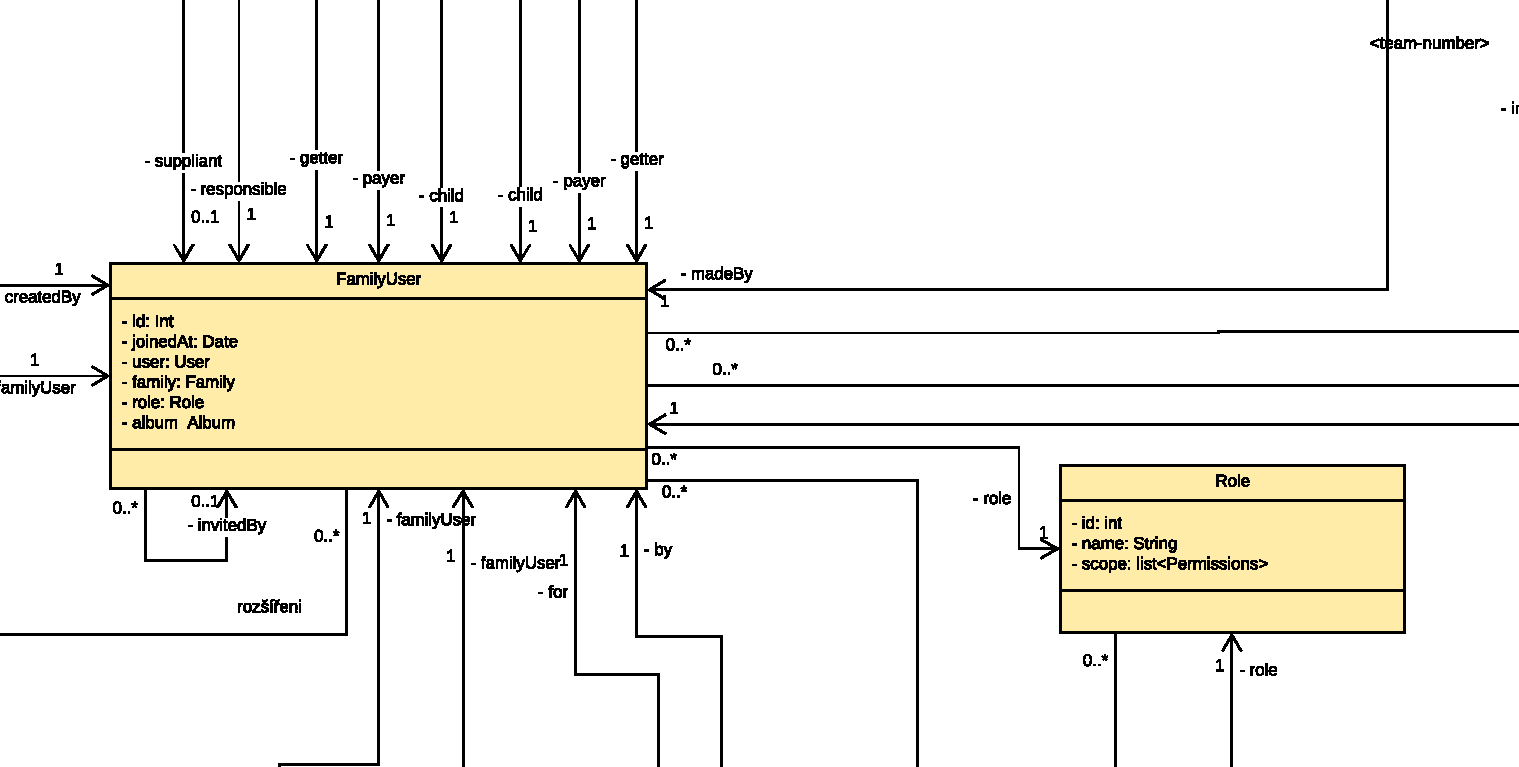
\includegraphics[width=0.7\textwidth]{pdfs/Role1}
	        \caption[Návrh \textit{Role}]{Návrh entity \textit{Role} podle Doménovém modelu z předmětu BI-SP2}\label{image:Role1}
        \end{figure}
    
    \subsection{Autorizace}
        Návrh bezpečné aplikace nebyl cílem předmětu zmíněných v sekcích \ref{analyza:navrh:sp1} a \ref{analyza:navrh:sp2}. Proto návrh a současná implementace neobsahuje proces přihlašovaní uživatele do systému. Nový procesu přihlašovaní bude zmíněn v sekci \ref{navrh:bezpecnost}.
        
    \subsection{Testování}
        Současný návrh neobsahuje informaci o implementaci testování. Současná implementace obsahuje jednu třídu, obsahující test, který se zaměřuje na ověření, zda se načetl {\textit{Context} aplikace}\footnote{Pokročilý kontejner, který funguje podobně \textit{BeanFactory}. Načítá definice beanů, provazuje je a vydává v případe nutnosti} (viz. obrázek \ref{code:test-context-loads1}).
        \begin{figure}
            \begin{minted}{java}
            @RunWith(SpringRunner::class)
            @SpringBootTest
            class RozvodyApplicationTests {

                @Test
                fun contextLoads() {
                }

            }
            \end{minted}
            \caption{Ukázka současného testování} 
            \label{code:test-context-loads1}
        \end{figure}

\chapter{Návrh}
V této kapitole bude popsán návrh backendu, který se skládá s současného návrhu, navržených změn a návrhu chybějící funkcionality.
\section{Navržené úpravy}\label{navrh:upravy}
    V teto sekce budou navrženy změny návrhu vzhledem k nedostatkům aktuálního návrhu, které byly nalezeny během vývoje backendové a forntendové částí aplikace. 
    \subsection{Interval}\label{narh:upravy:interval}
    První změnou je nový návrh entity Interval. Původní návrh (viz. obrázek \ref{image:Interval1}) nevyhovoval svojí složitostí a zároveň jenom částečným pokrytím možných případů. Podrobněji teto problém je popsán v sekci \ref{analyza:pozadavky-frontendu}. Entita interval byla rozdělena do dvou entit. První entita (viz. obrázek \ref{image:Interval2}) úplně nahrazuje původní entitu. Druhou entitou je \textit{CareDayInterval} (viz. obrázek \ref{image:careDayInterval}), která reprezentuje časové rozmezí pečovatelských dnů.
    \begin{figure}\centering
	    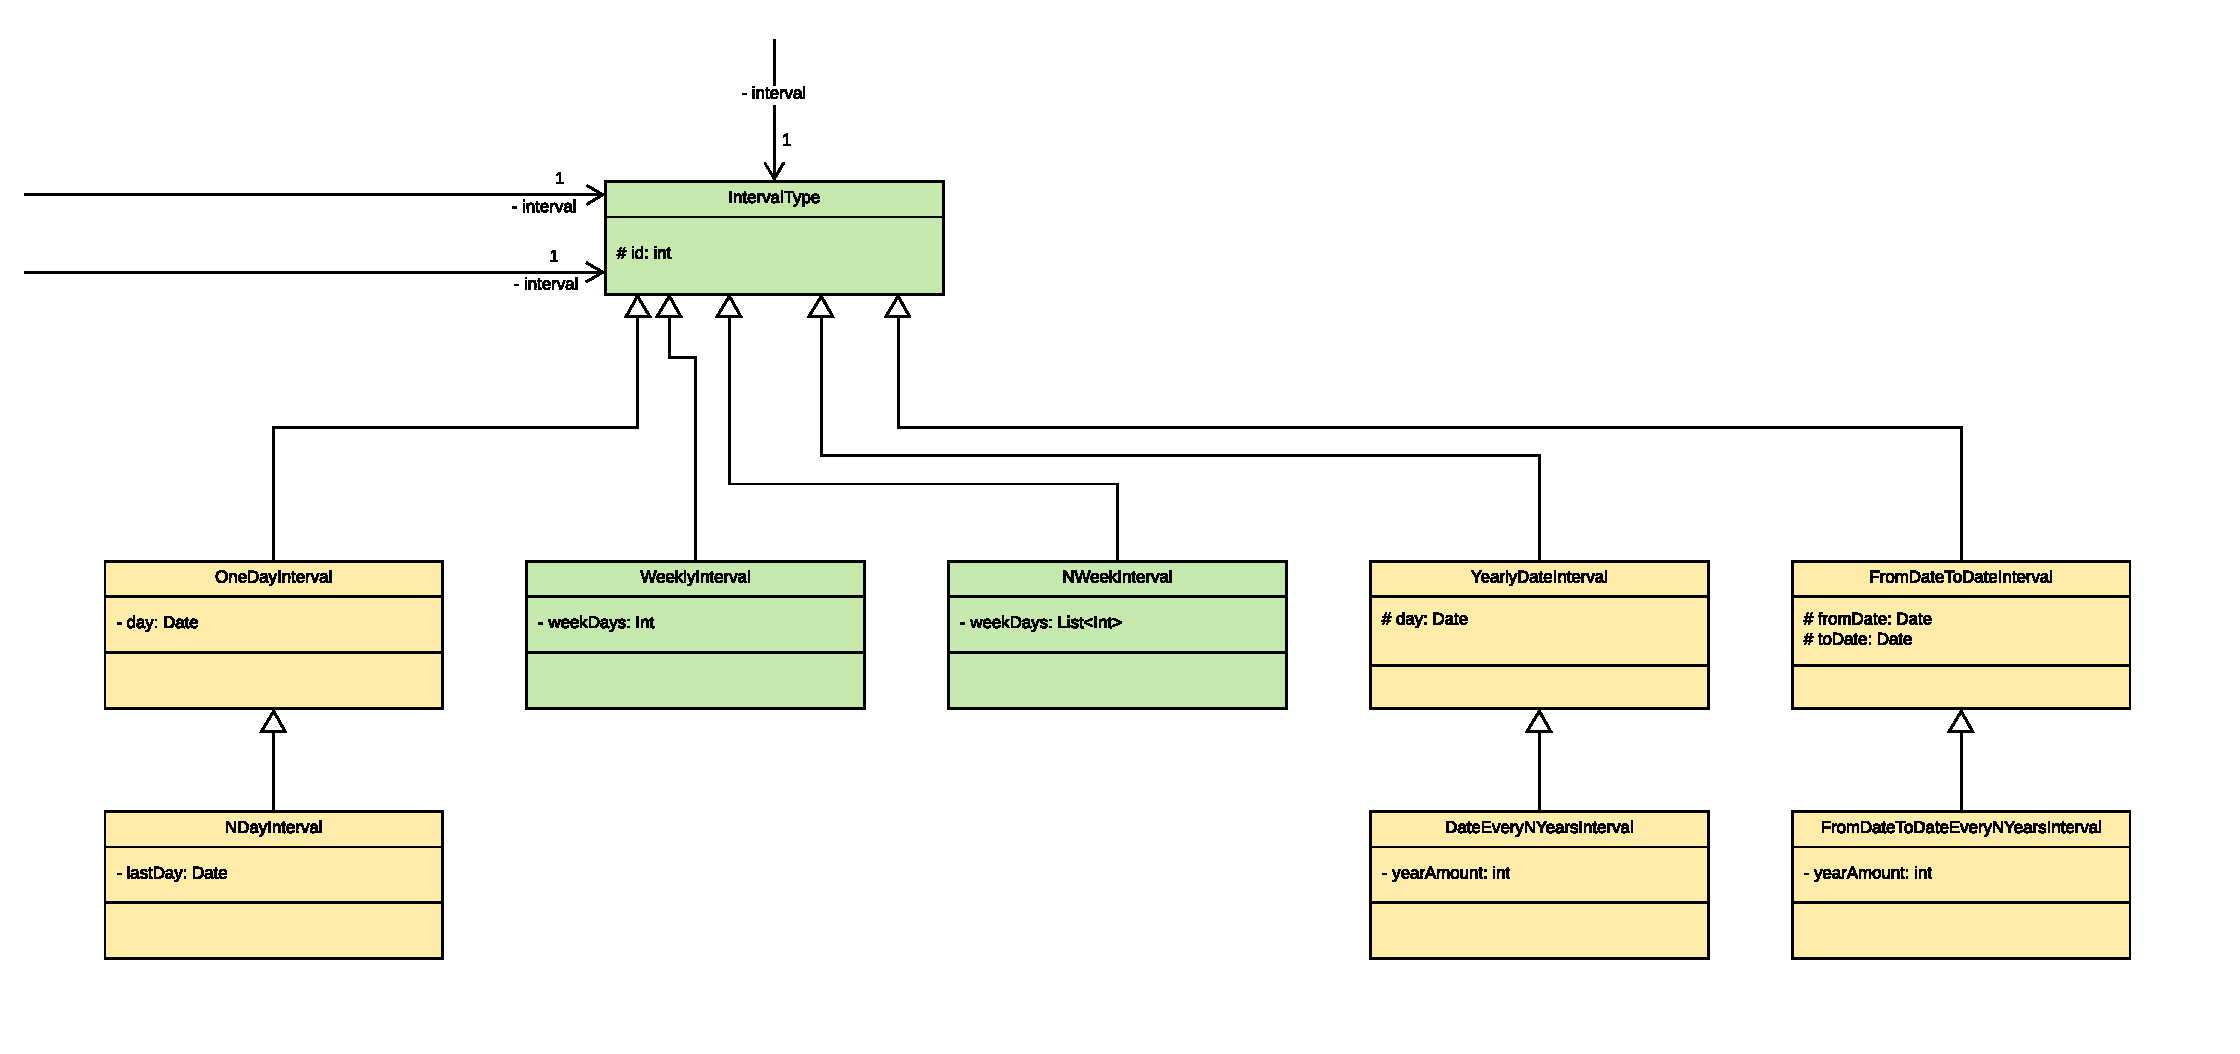
\includegraphics[width=1.0\textwidth]{pdfs/Interval1}
	    \caption[Návrh intervalu]{Návrh entity \textit{Interval} v Doménovém modelu z předmětu BI-SP2}\label{image:Interval1}
    \end{figure}
    \begin{figure}\centering
	    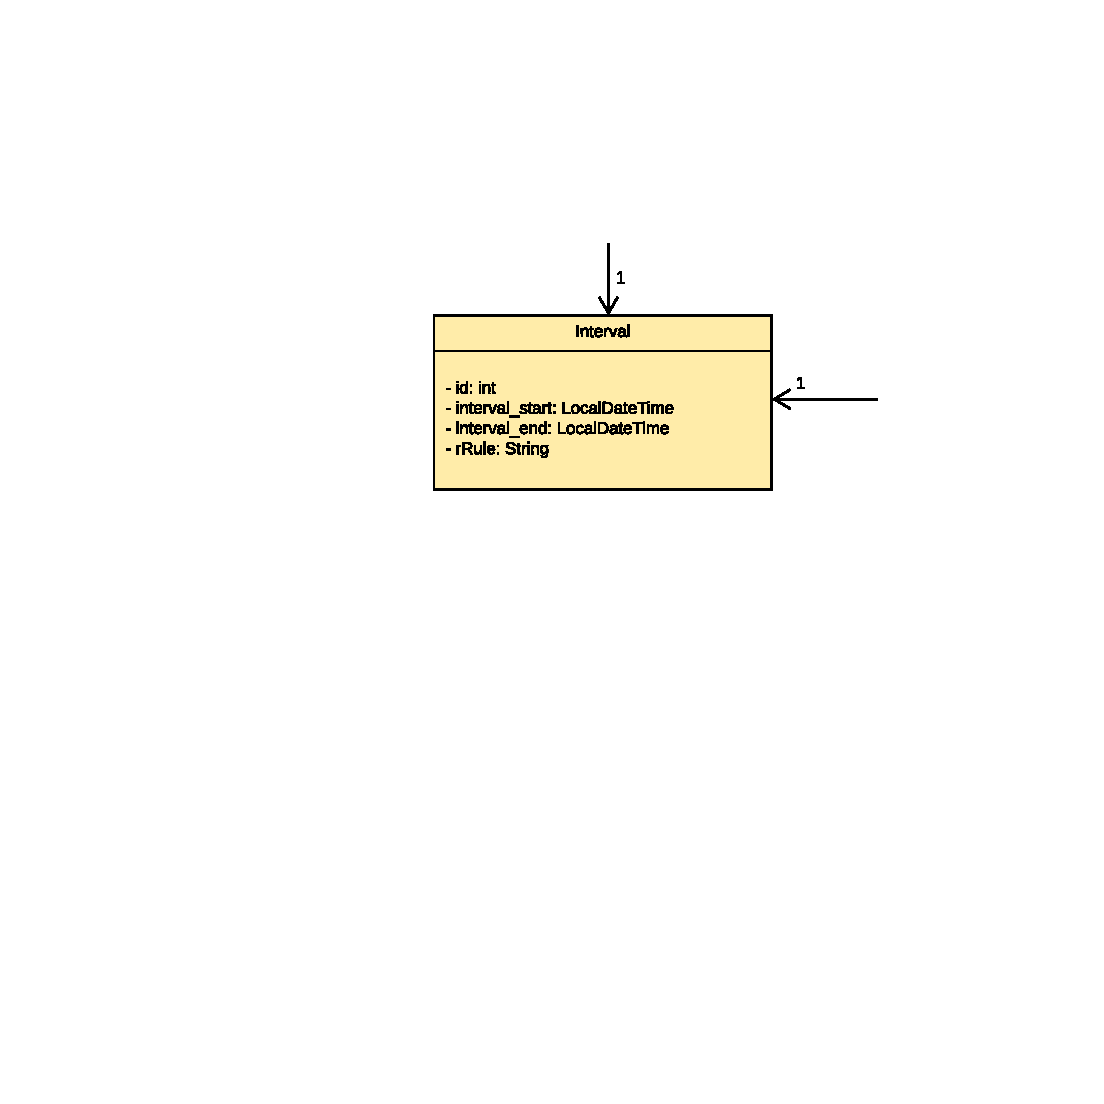
\includegraphics[width=0.5\textwidth]{pdfs/Interval2}
	    \caption[Návrh intervalu]{Nový návrh entity \textit{Interval}}\label{image:Interval2}
    \end{figure}
    \begin{figure}\centering
	    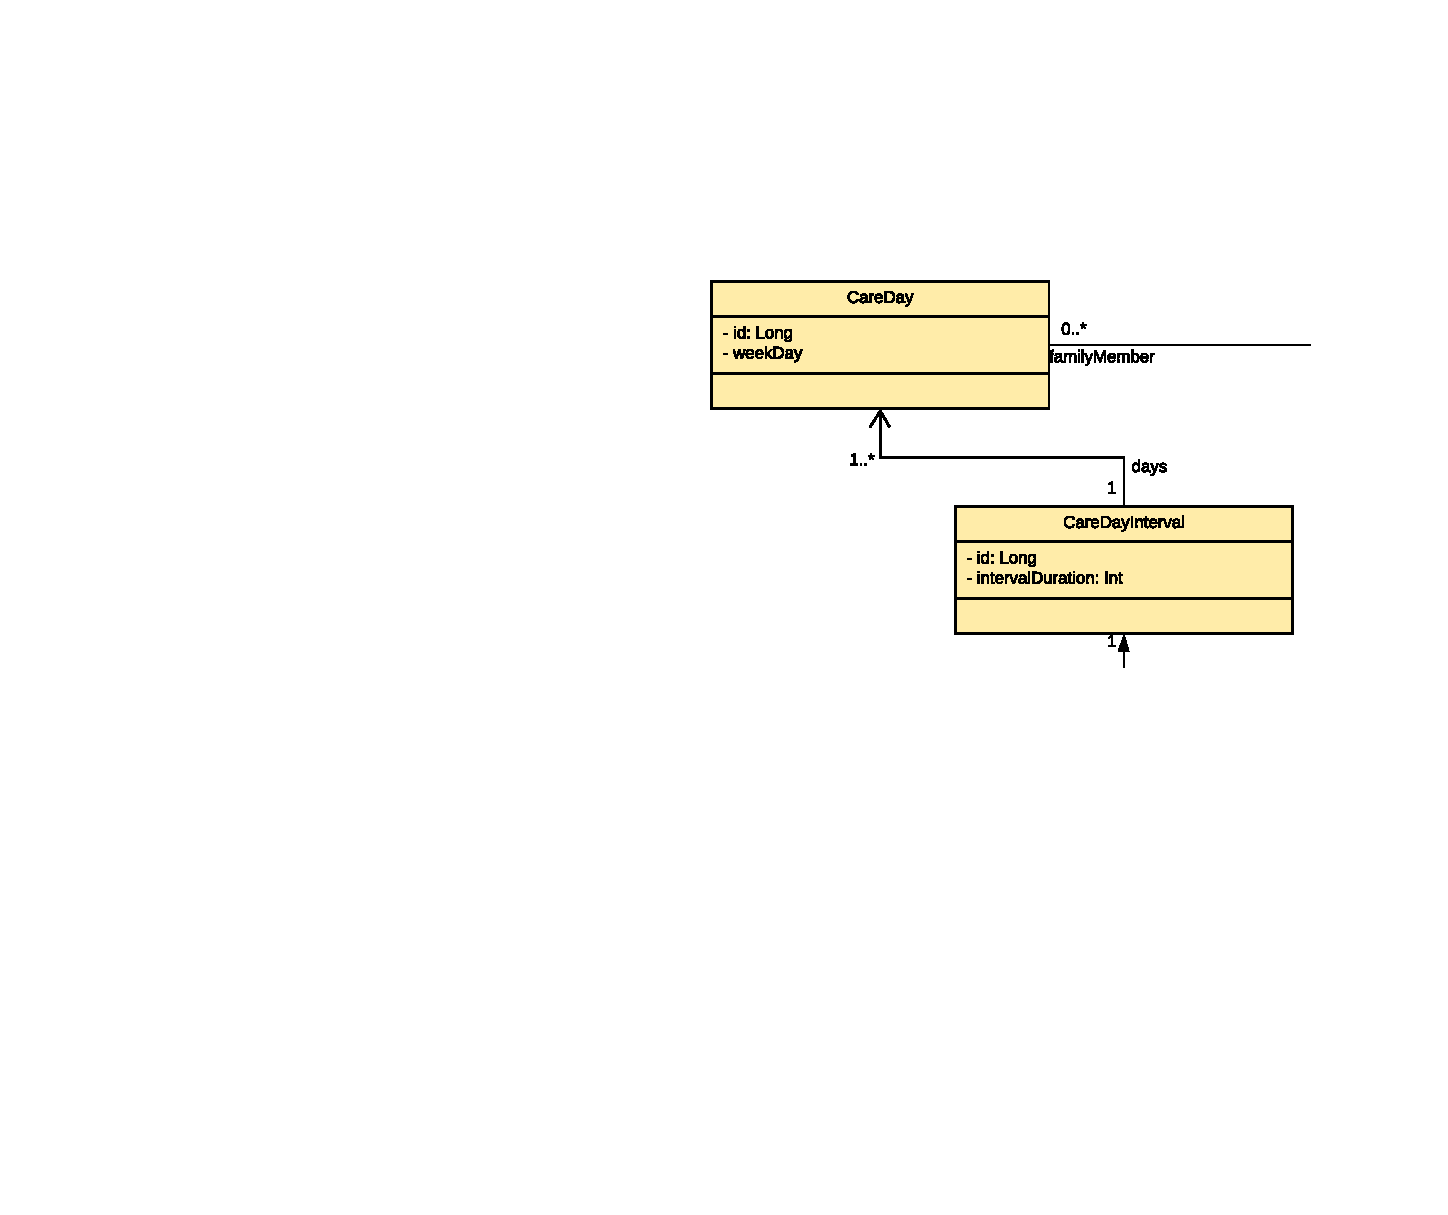
\includegraphics[width=0.5\textwidth]{pdfs/CareDayInterval}
	    \caption[Návrh intervalu]{Návrh entity \textit{CareDayInterval}}\label{image:careDayInterval}
    \end{figure}
    
    Nový návrh je postaven na úplně jiném principu. Časové rozmezí může být reprezentované dvěma způsoby. Oba dva způsoby vyžadují uvedení začátku intervalu. Tento parametr je povinný. První způsob, kromě začátku intervalu, vyžaduje i konec intervalu. Takovým způsobem můžeme definovat jednorázový interval po sobě jdoucích dnů. Druhý způsob vyžaduje zadání pravidlo opakování. Takhle můžeme definovat stejnou interval, ale mnohem složitějším způsobem. Na druhou stranu, pomocí takového pravidla můžeme definovat libovolně složitý interval. Takový návrh vyžaduje aby, buď byl zadán jenom konec intervalu, nebo bylo jenem zadáno pravidlo opakování. Pokud tyto dva parametry budou zadány najednou, server vyhodí chybu a zastaví vytvoření nesprávného intervalu.
    
    Pravidlo opakování je reprezentováno pomocí textového řetězce a má být zadáno ve standardu {RFC 5545}\cite{recurrence-rule}. Pro pohodlné testování byl navržen a implementován {interní DSL jazyk}\footnote{programovací jazyk nebo použití obecného programovacího jazyku, vytvořený za účelem vyřešení konkretní problémové domény}, který nadává možnost vytvořit pravidlo opakovaní. Dále uvádím příklad \textit{Intervalu}, který má pravidlo opakování vytvořené pomoci DSL jazyku. Tento interval bude použit při testování.
    \begin{figure}
        \begin{minted}{java}
        /**
        * Valid Interval with recurrence rule.
        */
        private val validInterval = Interval(
                id = 1,
                interval_start = creationTime,
                interval_end = null,
                rRule = rule(frequency = Frequency.WEEKLY, count = 10) {
                    byDays {
                        and(DayOfWeek.MONDAY)
                        and(DayOfWeek.WEDNESDAY)
                        and(DayOfWeek.SUNDAY)
                    }
                }
        )
        \end{minted}
        \caption{Ukázka \textit{Intervalu} s pravidlem opakování} 
        \label{code:valid-interval}
        \end{figure}
        %TODO popsat implemenaci interniho DSL
\section{Navrh bezpečnosti}\label{navrh:bezpecnost}

\section{Návrh testování}\label{navrh:testovani}
    Pro testování kódu budou využity frameworky JUnit 5 a Spring. Podrobný popis těchto frameworků byl v sekci \ref{resere:testovani}. Testování se skládá s \textit{Unit}\footnote{testy, zaměřené na ověření správnosti } testů a \textit{Integration}\footnote{TODO} testů.

% \chapter{Implementace}

% \section{Dokumentace API}
% \section{Intervaly}
% \section{Profily aplikace}
% Aplikace má root uźivatele, který by neměl vyskytovat v produkce.
% \section{Bezpečnost}

\chapter{Testování}\label{testovani}
% Nedílnou součástí vývoje softwaru je testování. Testování bylo rozděleno do dvou vrstev. Základní vrstvou jsou unit testy. Pro tvorbu těchto testů byl použit framework JUnit 5. Druhou vrstvou jsou integrační testy, které jsou implementovány pomoci funkcionality, kterou poskytuje framework Spring.
V teto kapitole bude popsán proces testování, doplňková funkcionalita, zjednodušující proces testování a také popis pokrytí kódů testy.
\section{Tagy}\label{testovani:tagy}
    TODO popis tagu a jejich implementace
    % Během vývoje velkých projektů zpouštění testů je významným problémem pro programátory. 
    % Framework JUnit 5 poskytuje možnost označovat metody a třídy pomocí tagu.
\section{Zobrazování testů}\label{testovani:zobrazovani}
    TODO popis CamelCaseGeneratoru a displayname
\section{Integrační testy}\label{testovani:intergacni}
    TODO podrobny popis
\section{Unit testy}\label{testovani:unit}
    TODO podrobny popis
\section{Pokrytí kódu testy}\label{testovani:pokryti}
    TODO V teto sekci je uveden popis provedéní analýzy pokrýtí kódu testy.
    % TODO smazat subsection pokud nebude pridan jeste jeden
    \subsection{JoCoCo}
    TODO pokryti kodu testy podle jacoco
    \cite{JoCoCo}
    % vestaveny junit engine v IntelifIDEA prestal fingovat po dosazeni velkeho poctu testu
    % \subsection{IntelliJ IDEA code coverage runner}
    % \cite{IntelliJ IDEA code coverage runner}

\input{tex/60_budouci_kroky}

\begin{conclusion}
	%space 1
%space 2 I hate this box on the top right corner
Projekt byl rozdělen do dvou samostatných častí, které byly vyvíjeny paralelně. První částí je Android aplikace. Druhou částí, která je předmětem této bakalářské práce, je serverový backend, poskytující RESTové služby pro Android aplikace.

Cílem této práce bylo navržení vhodných úprav a následná implementace existujícího návrhu a fragmentů implementace. Také zhodnocení použitelnosti výsledné implementace a navržení vhodných budoucích kroků pro pokračování vývoje serveru. Při implementaci byl také uvažován současný stav souběžně vyvíjené, frontendové části aplikace.

I~když se autor této práce zúčastnil předmětů, během kterých byl udělán předchozí návrh aplikace a fragmenty implementace, byla potřeba přezkoumat návrh programu za účelem vylepšení návrhu a eliminování nalezených nedostatků během implementace frontendové a backendové části. Předchozí implementace programu pokrývala jenom malou část aplikace, proto skoro celá již existující implementace byla přepsána. Byl opraven doménový model, provedeny změny použité třívrstvé architektury, rozšířené API, rozšířená dokumentace API, přidán proces registrace a přihlašování uživatele a také byla implementována bezpečnost aplikace. Při implementaci byly uvazovány požadavky kolegy, který souběžně vyvíjí frontendovou část aplikace.

% Práce se začíná analýzou existujícího návrhu a fragmentů implementace. I když jsem zúčastnil předmětů, které se zabývali těmto návrhem a implementací, potřeboval jsem přezkoumat celý návrh za účelem eliminování, nalezených během implementace frontendové a backendové častí, nedostatků a navržení lepších řešení.
% Potom jsem návrh novou verzí řešení, která obsahuje úpravy podle požadavků frontendové části aplikace a zároveň obsahuje navržené mnou úpravy. Implementace navrženého řešení byla nejsložitější častí této bakalářské práci, protože jsem neměl zkušeností ve vývoje projektů porovnatelného rozsahu a potřeboval jsem naučit mnoha novým věcem.
Důležitou částí této práce bylo testování, které je v~rozsahu napsaného kódu porovnatelné s~implementací serveru samotného. Testy byly rozděleny do dvou typů: unit testy a integrační testy. Unit testy testují samostatně testovatelné funkce programu. Integrační testy využívají za běhu celý kontext aplikace a testují, jestli jednotlivé řadiče fungují správně. 
% \begin{figure}\centering
% 	   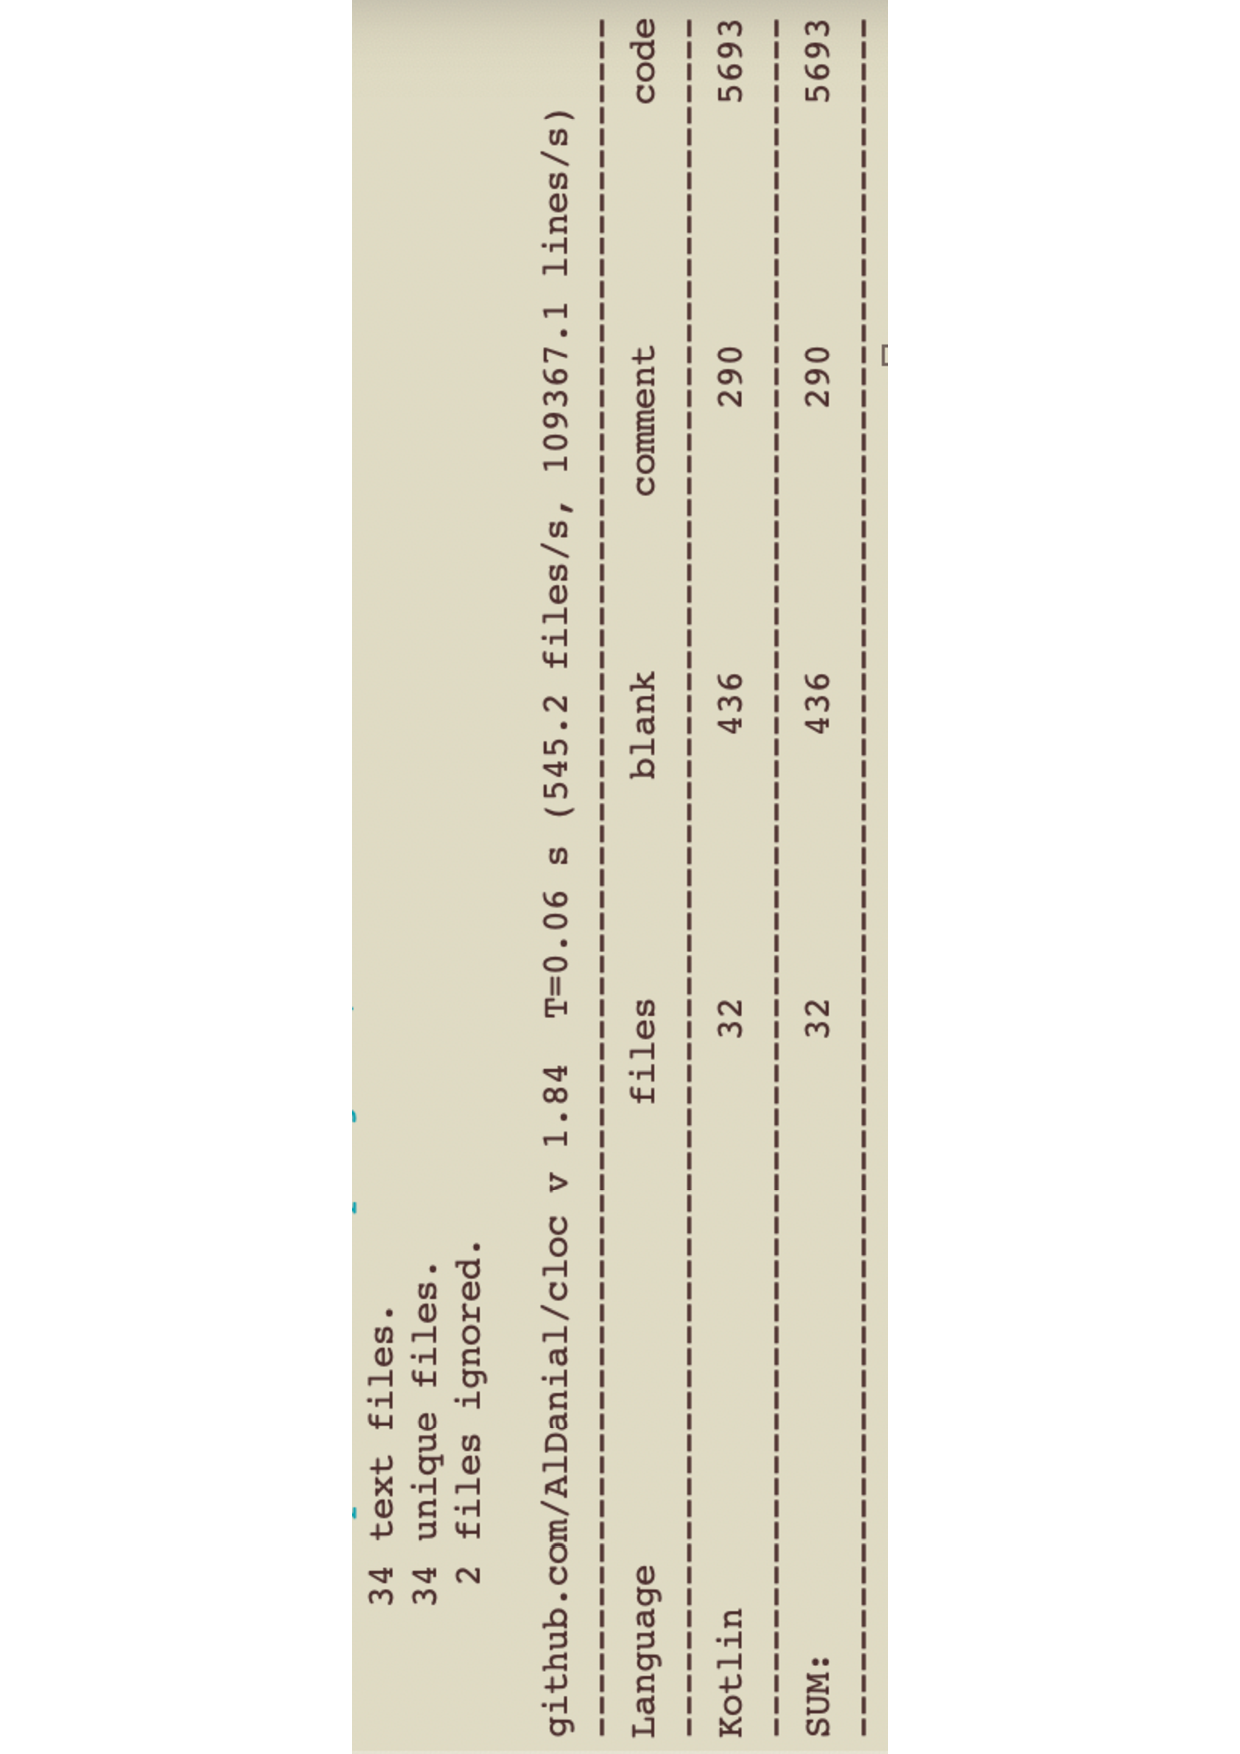
\includegraphics[angle=-90, width=0.5\textwidth]{pdfs/CodeAmountTests2}
% 	   \caption[Analýza kódu testů]{Počet napsáných řádek kódu testů}\label{image:code-count-test}
% \end{figure}
% \begin{figure}\centering
% 	   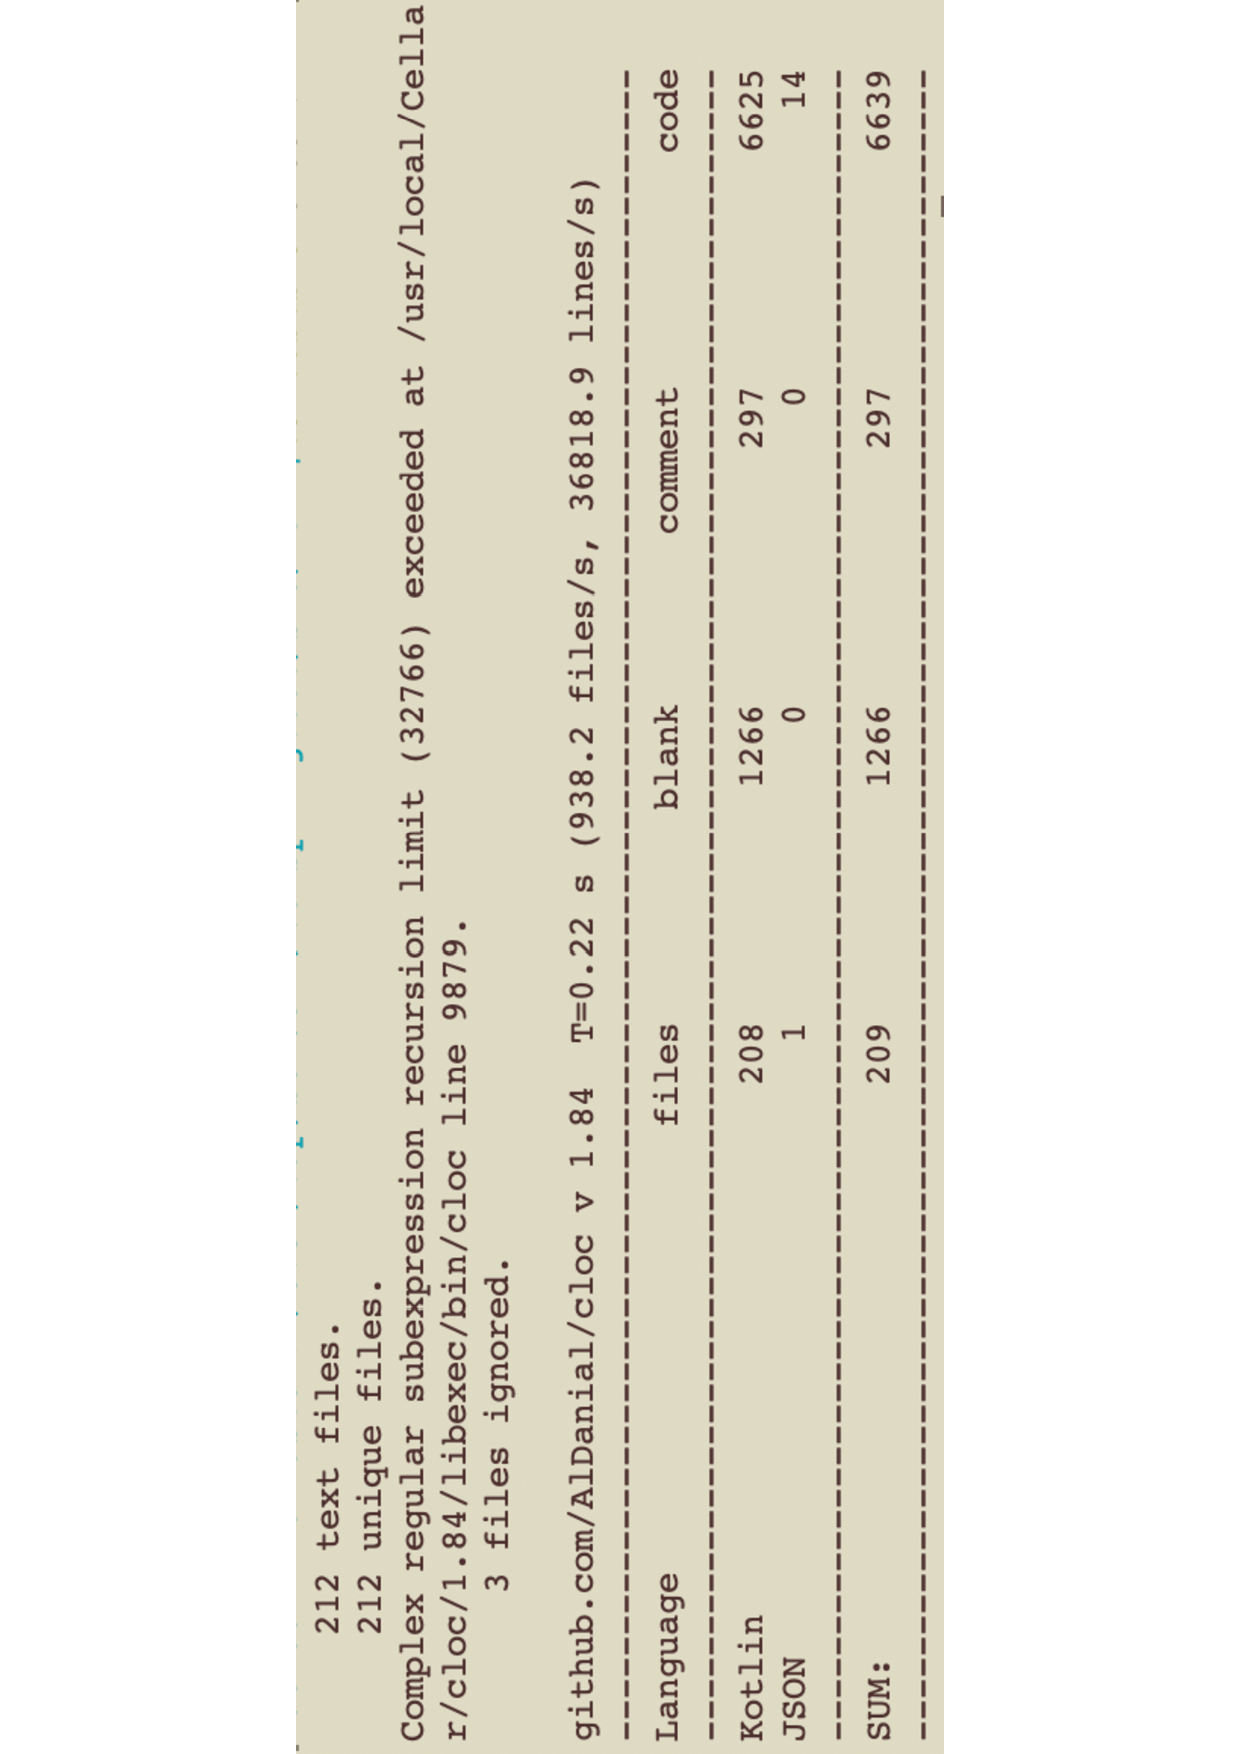
\includegraphics[angle=-90, width=0.5\textwidth]{pdfs/CodeAmountImpl2}
% 	   \caption[Analýza kódu implementace]{Počet napsáných řádek kódu za účelem implementace funkcionality}\label{image:code-count-main}
% \end{figure}

Výsledkem této bakalářské práce je funkční aplikace splňující všechny požadavky frontendové části aplikace. Ale, jak Android aplikace, tak i serverový backend ještě nejsou ve svém finálním stavu. V~rámci této práce byl zhodnocen současný stav a představeny vhodné budoucí kroky pro pokračování vývoje.
% Následující kapitola se věnuje zhodnocení použitelností výsledné implementace a navržení budoucích kroků. Výsledek ještě není připravený pro produkční prostředí a ještě ho očekává dostatečný počet vylepšení. V rámci této bakalářské práci jsem implementoval základ backendu, který má skoro celou potřebnou funkcionalitu, kromě některých věcí, které byly objevený už během pečlivého zanoření do implementace a za
% řazené do budoucích kroků.
\end{conclusion}

% \bibliographystyle{csn690}
% \bibliography{mybibliographyfile}
% \printbibliography


\printbibliography

\appendix

\chapter{Seznam použitých zkratek}
\begin{description}
    \item[API] Application Programming Interface
    \item[BI-SP1] Bakalářský předmět Softwarový týmový projekt 1 vyučovaný na FIT ČVUT
    \item[BI-SP2] Bakalářský předmět Softwarový týmový projekt 2 vyučovaný na FIT ČVUT
    \item[CLOC] Count Lines of Code
    \item[ČVUT] České vysoké učení technické v Praze
    \item[DSL] Domain-Specific Language
    \item[DTO] Data Transfer Object
    \item[FIT] Fakulta informačních technologií
    \item[HTML] Hypertext Markup Language
    \item[HTTP] Hypertext Transfer Protocol
    \item[HTTPS] Hypertext Transfer Protocol Secure 
    \item[ID] Identifikátor
    \item[IoC] Inversion of Control
    \item[JVM] Java Virtual Machine
    \item[REST] Representational State Transfer
    \item[SQL] Structured Query Language 
    \item[URI] Uniform Resource Identifier
\end{description}

\chapter{Slovník pojmů}
\begin{description}[leftmargin=12em,style=nextline] % TODO dodelat vsechny, upravit do spravneho poradi 
    \item[Framework] Framework je softwarová struktura orientovaná na vyřešení problému nebo jeho zjednodušení při procesu vývoje softwarových projektu
	\item[Backend] Část aplikace, která se stará o data a jejích spravování. Pro interakci s backendem klient většinou potřebuje přistup do frontendové části aplikace
    \item[Frontend] Prezentáční vrstva aplikace se kterou interaguje klient. 
	\item[DSL jazyk] Programovací jazyk nebo použití obecného programovacího jazyku, vytvořený za účelem vyřešení konkretní problémové domény
	\item[Interní DSL jazyk] DSL jazyk využívající obecný programovací jazyk
	\item[Unit testy] Testy, zaměřené na ověření správnosti fungování samostatně testovatelné části programu
	\item[Integrační testy] Testy, zaměřené na ověření správné komunikace mezi komponentami
	\item[Inversion of Controle] Princip, za kterého kontrola nad vytvořením a provázáním tříd vlastní framework. 
	\item[Git]  Git je distribuovaný systém řízení verzí
	\item[Commit]  Commit je proces při kterém se uloží všechny udělané v rámci systému řízení verzí změny a zařadí se do historie změn
	\item[GitLab] GitLab je webový platformou pro vývoj softwaru pomocí systému řízení verzí Git
	\item[Diagram Užití] Diagram Užití popisuje chování systému z vnějšího pohledu
	\item[Diagram aktivit] Diagram aktivit zobrazuje jak objekty spolupracují
	\item[Wireframe] Wireframy je grafické zobrazení hlavních prvků frontendové častí aplikace
	\item[Doménový model] Doménový model je náčrtem základních entit systému a vztahů mezi nimi
	\item[CLOC] Nástroj poskytující možnost spočítat počet řádek kódu v dáne složce. Nástroj podporuje velký počet jazyku programování. Výsledek obsahuje počet řádek kódu oddělený od komentářů a prázdných řádků.
	\item[mapování] Proces přidání konkrétnímu controlleru adresy pomocí anotací frameworku Spring, která se zadává jako URI při odesílaní požadavků na Server
	\item[Kontext aplikace] Pokročilý kontejner, který funguje podobně \textit{BeanFactory}. Načítá definice beanů, provazuje je a vydává v případe nutnosti
\end{description}


% % % % % % % % % % % % % % % % % % % % % % % % % % % % 
% % Tuto kapitolu z výsledné práce ODSTRAŇTE.
% % % % % % % % % % % % % % % % % % % % % % % % % % % % 
% 
% \chapter{Návod k~použití této šablony}
% 
% Tento dokument slouží jako základ pro napsání závěrečné práce na Fakultě informačních technologií ČVUT v~Praze.
% 
% \section{Výběr základu}
% 
% Vyberte si šablonu podle druhu práce (bakalářská, diplomová), jazyka (čeština, angličtina) a kódování (ASCII, \mbox{UTF-8}, \mbox{ISO-8859-2} neboli latin2 a nebo \mbox{Windows-1250}). 
% 
% V~české variantě naleznete šablony v~souborech pojmenovaných ve formátu práce\_kódování.tex. Typ může být:
% \begin{description}
% 	\item[BP] bakalářská práce,
% 	\item[DP] diplomová (magisterská) práce.
% \end{description}
% Kódování, ve kterém chcete psát, může být:
% \begin{description}
% 	\item[UTF-8] kódování Unicode,
% 	\item[ISO-8859-2] latin2,
% 	\item[Windows-1250] znaková sada 1250 Windows.
% \end{description}
% V~případě nejistoty ohledně kódování doporučujeme následující postup:
% \begin{enumerate}
% 	\item Otevřete šablony pro kódování UTF-8 v~editoru prostého textu, který chcete pro psaní práce použít -- pokud můžete texty s~diakritikou normálně přečíst, použijte tuto šablonu.
% 	\item V~opačném případě postupujte dále podle toho, jaký operační systém používáte:
% 	\begin{itemize}
% 		\item v~případě Windows použijte šablonu pro kódování \mbox{Windows-1250},
% 		\item jinak zkuste použít šablonu pro kódování \mbox{ISO-8859-2}.
% 	\end{itemize}
% \end{enumerate}
% 
% 
% V~anglické variantě jsou šablony pojmenované podle typu práce, možnosti jsou:
% \begin{description}
% 	\item[bachelors] bakalářská práce,
% 	\item[masters] diplomová (magisterská) práce.
% \end{description}
% 
% \section{Použití šablony}
% 
% Šablona je určena pro zpracování systémem \LaTeXe{}. Text je možné psát v~textovém editoru jako prostý text, lze však také využít specializovaný editor pro \LaTeX{}, např. Kile.
% 
% Pro získání tisknutelného výstupu z~takto vytvořeného souboru použijte příkaz \verb|pdflatex|, kterému předáte cestu k~souboru jako parametr. Vhodný editor pro \LaTeX{} toto udělá za Vás. \verb|pdfcslatex| ani \verb|cslatex| \emph{nebudou} s~těmito šablonami fungovat.
% 
% Více informací o~použití systému \LaTeX{} najdete např. v~\cite{wikilatex}.
% 
% \subsection{Typografie}
% 
% Při psaní dodržujte typografické konvence zvoleného jazyka. České \uv{uvozovky} zapisujte použitím příkazu \verb|\uv|, kterému v~parametru předáte text, jenž má být v~uvozovkách. Anglické otevírací uvozovky se v~\LaTeX{}u zadávají jako dva zpětné apostrofy, uzavírací uvozovky jako dva apostrofy. Často chybně uváděný symbol "{} (palce) nemá s~uvozovkami nic společného.
% 
% Dále je třeba zabránit zalomení řádky mezi některými slovy, v~češtině např. za jednopísmennými předložkami a spojkami (vyjma \uv{a}). To docílíte vložením pružné nezalomitelné mezery -- znakem \texttt{\textasciitilde}. V~tomto případě to není třeba dělat ručně, lze použít program \verb|vlna|.
% 
% Více o~typografii viz \cite{kobltypo}.
% 
% \subsection{Obrázky}
% 
% Pro umožnění vkládání obrázků je vhodné použít balíček \verb|graphicx|, samotné vložení se provede příkazem \verb|\includegraphics|. Takto je možné vkládat obrázky ve formátu PDF, PNG a JPEG jestliže používáte pdf\LaTeX{} nebo ve formátu EPS jestliže používáte \LaTeX{}. Doporučujeme preferovat vektorové obrázky před rastrovými (vyjma fotografií).
% 
% \subsubsection{Získání vhodného formátu}
% 
% Pro získání vektorových formátů PDF nebo EPS z~jiných lze použít některý z~vektorových grafických editorů. Pro převod rastrového obrázku na vektorový lze použít rasterizaci, kterou mnohé editory zvládají (např. Inkscape). Pro konverze lze použít též nástroje pro dávkové zpracování běžně dodávané s~\LaTeX{}em, např. \verb|epstopdf|.
% 
% \subsubsection{Plovoucí prostředí}
% 
% Příkazem \verb|\includegraphics| lze obrázky vkládat přímo, doporučujeme však použít plovoucí prostředí, konkrétně \verb|figure|. Například obrázek \ref{fig:float} byl vložen tímto způsobem. Vůbec přitom nevadí, když je obrázek umístěn jinde, než bylo původně zamýšleno -- je tomu tak hlavně kvůli dodržení typografických konvencí. Namísto vynucování konkrétní pozice obrázku doporučujeme používat odkazování z~textu (dvojice příkazů \verb|\label| a \verb|\ref|).
% 
% \begin{figure}\centering
% 	
\includegraphics[width=0.5\textwidth, angle=30]{cvut-logo-bw}
% 	\caption[Příklad obrázku]{Ukázkový obrázek v~plovoucím prostředí}\label{fig:float}
% \end{figure}
% 
% \subsubsection{Verze obrázků}
% 
% % Gnuplot BW i barevně
% Může se hodit mít více verzí stejného obrázku, např. pro barevný či černobílý tisk a nebo pro prezentaci. S~pomocí některých nástrojů na generování grafiky je to snadné.
% 
% Máte-li například graf vytvořený v programu Gnuplot, můžete jeho černobílou variantu (viz obr. \ref{fig:gnuplot-bw}) vytvořit parametrem \verb|monochrome dashed| příkazu \verb|set term|. Barevnou variantu (viz obr. \ref{fig:gnuplot-col}) vhodnou na prezentace lze vytvořit parametrem \verb|colour solid|.
% 
% \begin{figure}\centering
% 	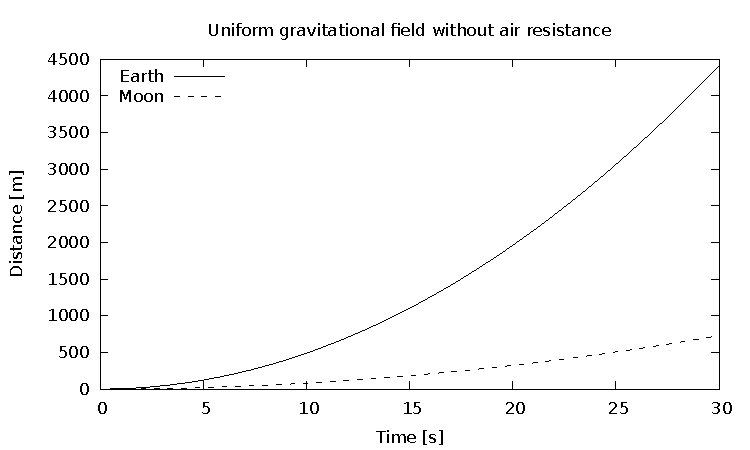
\includegraphics{gnuplot-bw}
% 	\caption{Černobílá varianta obrázku generovaného programem Gnuplot}\label{fig:gnuplot-bw}
% \end{figure}
% 
% \begin{figure}\centering
% 	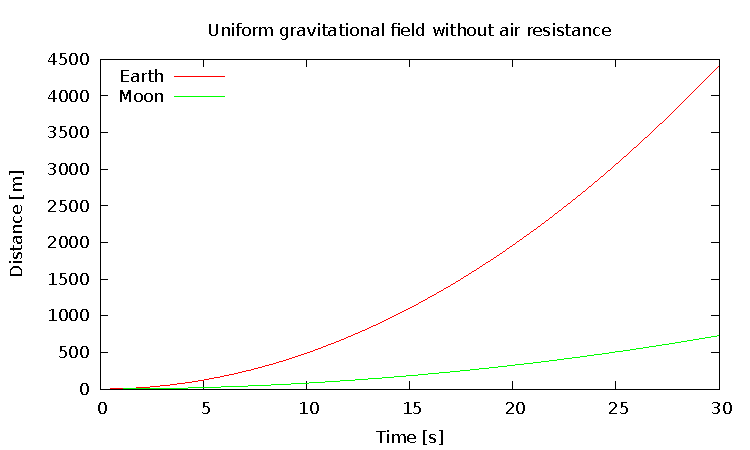
\includegraphics{gnuplot-col}
% 	\caption{Barevná varianta obrázku generovaného programem Gnuplot}\label{fig:gnuplot-col}
% \end{figure}
% 
% 
% \subsection{Tabulky}
% 
% Tabulky lze zadávat různě, např. v~prostředí \verb|tabular|, avšak pro jejich vkládání platí to samé, co pro obrázky -- použijte plovoucí prostředí, v~tomto případě \verb|table|. Například tabulka \ref{tab:matematika} byla vložena tímto způsobem.
% 
% \begin{table}\centering
% 	\caption[Příklad tabulky]{Zadávání matematiky}\label{tab:matematika}
% 	\begin{tabular}{|l|l|c|c|}\hline
% 		Typ		& Prostředí		& \LaTeX{}ovská zkratka	& \TeX{}ovská zkratka	\tabularnewline \hline \hline
% 		Text		& \verb|math|		& \verb|\(...\)|	& \verb|$...$|		\tabularnewline \hline
% 		Displayed	& \verb|displaymath|	& \verb|\[...\]|	& \verb|$$...$$|	\tabularnewline \hline
% 	\end{tabular}
% \end{table}
% 
% % % % % % % % % % % % % % % % % % % % % % % % % % % % 

% TODO uploudovat posledni verzi domenoveho modelu
\chapter{Doménový model před úpravami}\label{dodatek:DomainModel}
    \begin{figure}\centering
	    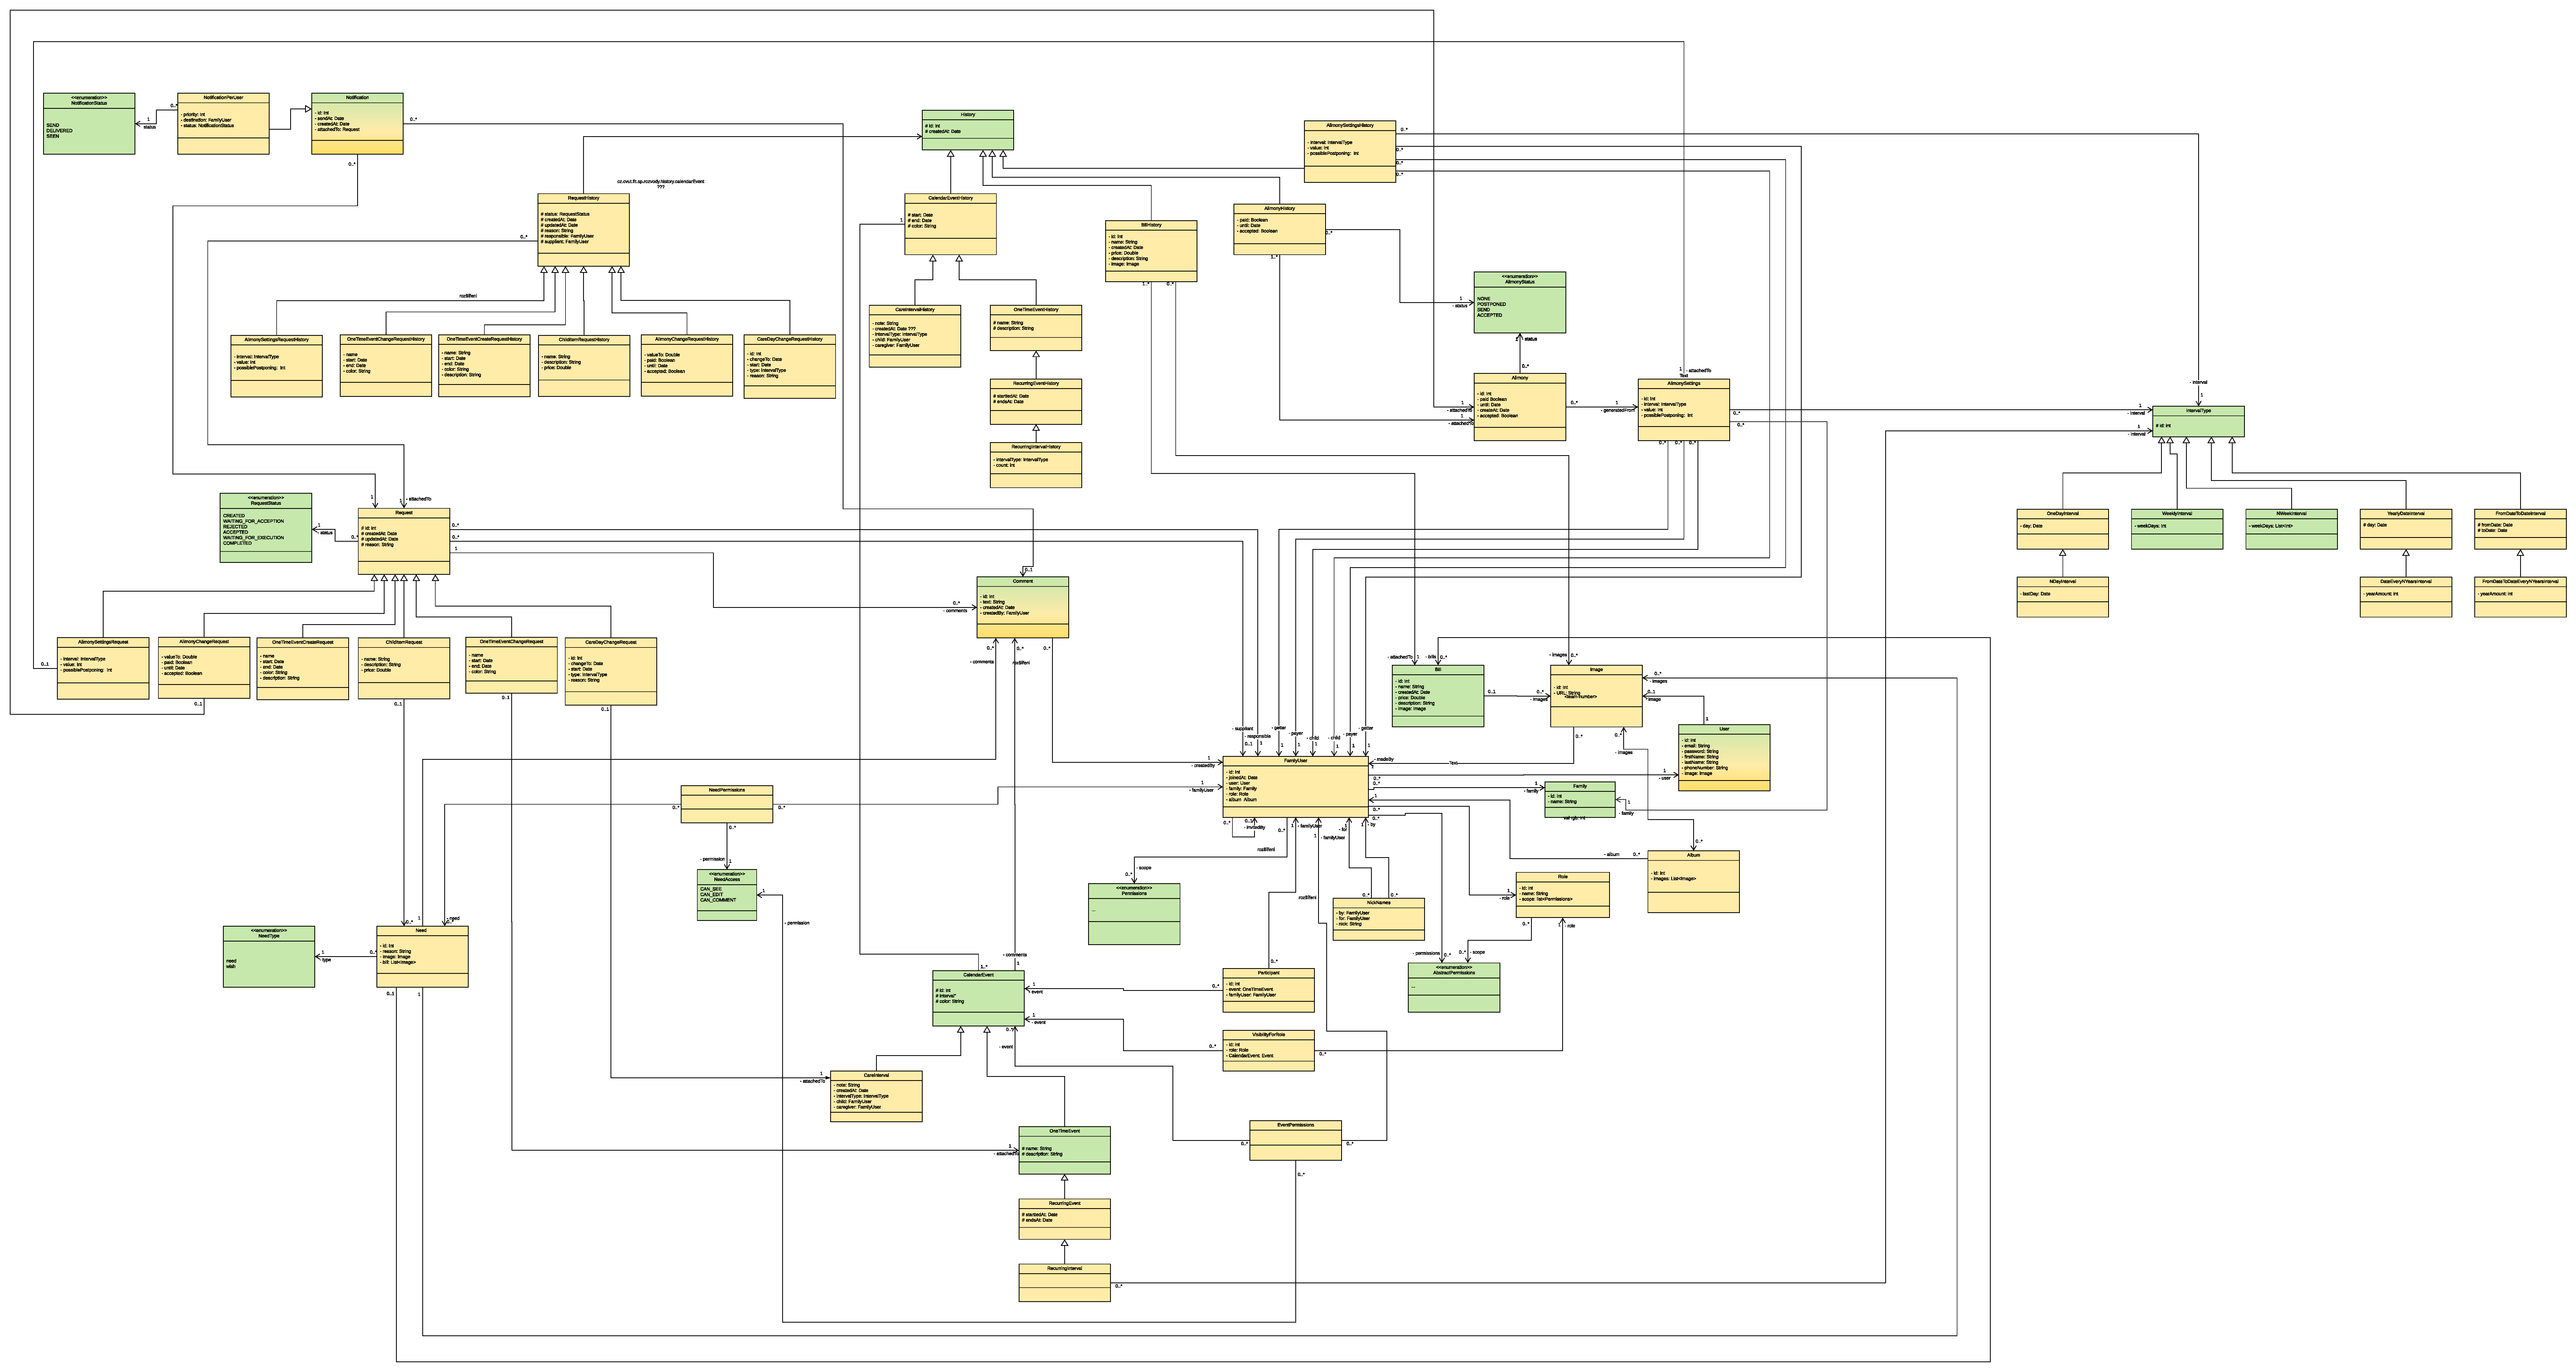
\includegraphics[angle=90, height=0.9\textheight]{pdfs/Domain-Model}
	    \caption[Doménový model před úpravami]{Doménový model z předmětu BI-SP2}\label{image:DomainModel}
    \end{figure}

\chapter{Testování}\label{dodatek:testing}
% \chapter{Pokrytí kódů testy}\label{dodatek:code-coverage}
    \begin{figure}\centering
	    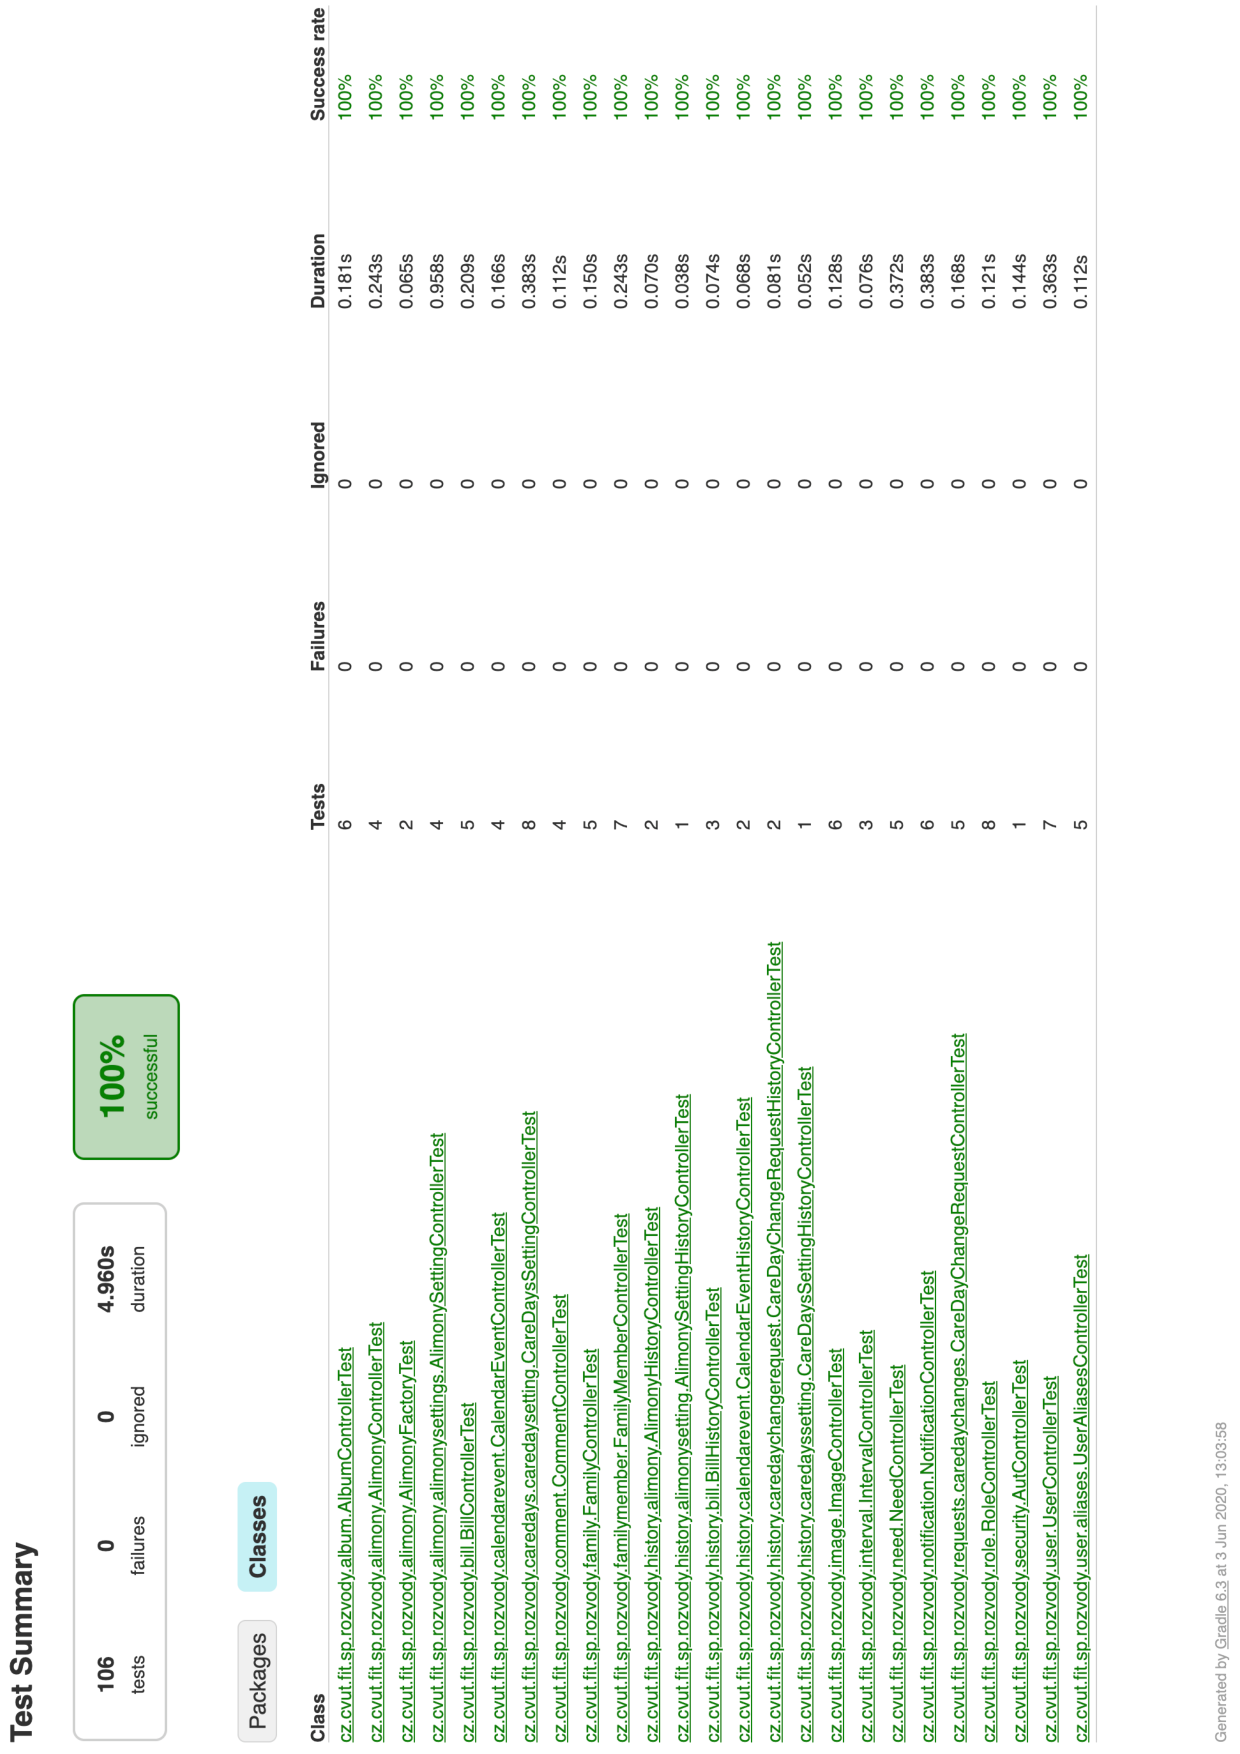
\includegraphics[width=1.0\textwidth]{pdfs/Gradle-unit-tests}
	    \caption[Seznam tříd obsahujících unit testy]{Seznam tříd obsahujících unit testy vygenerovaný pomocí nástroje Gradle}\label{image:gradle-unit-tests}
    \end{figure}
    \begin{figure}\centering
	    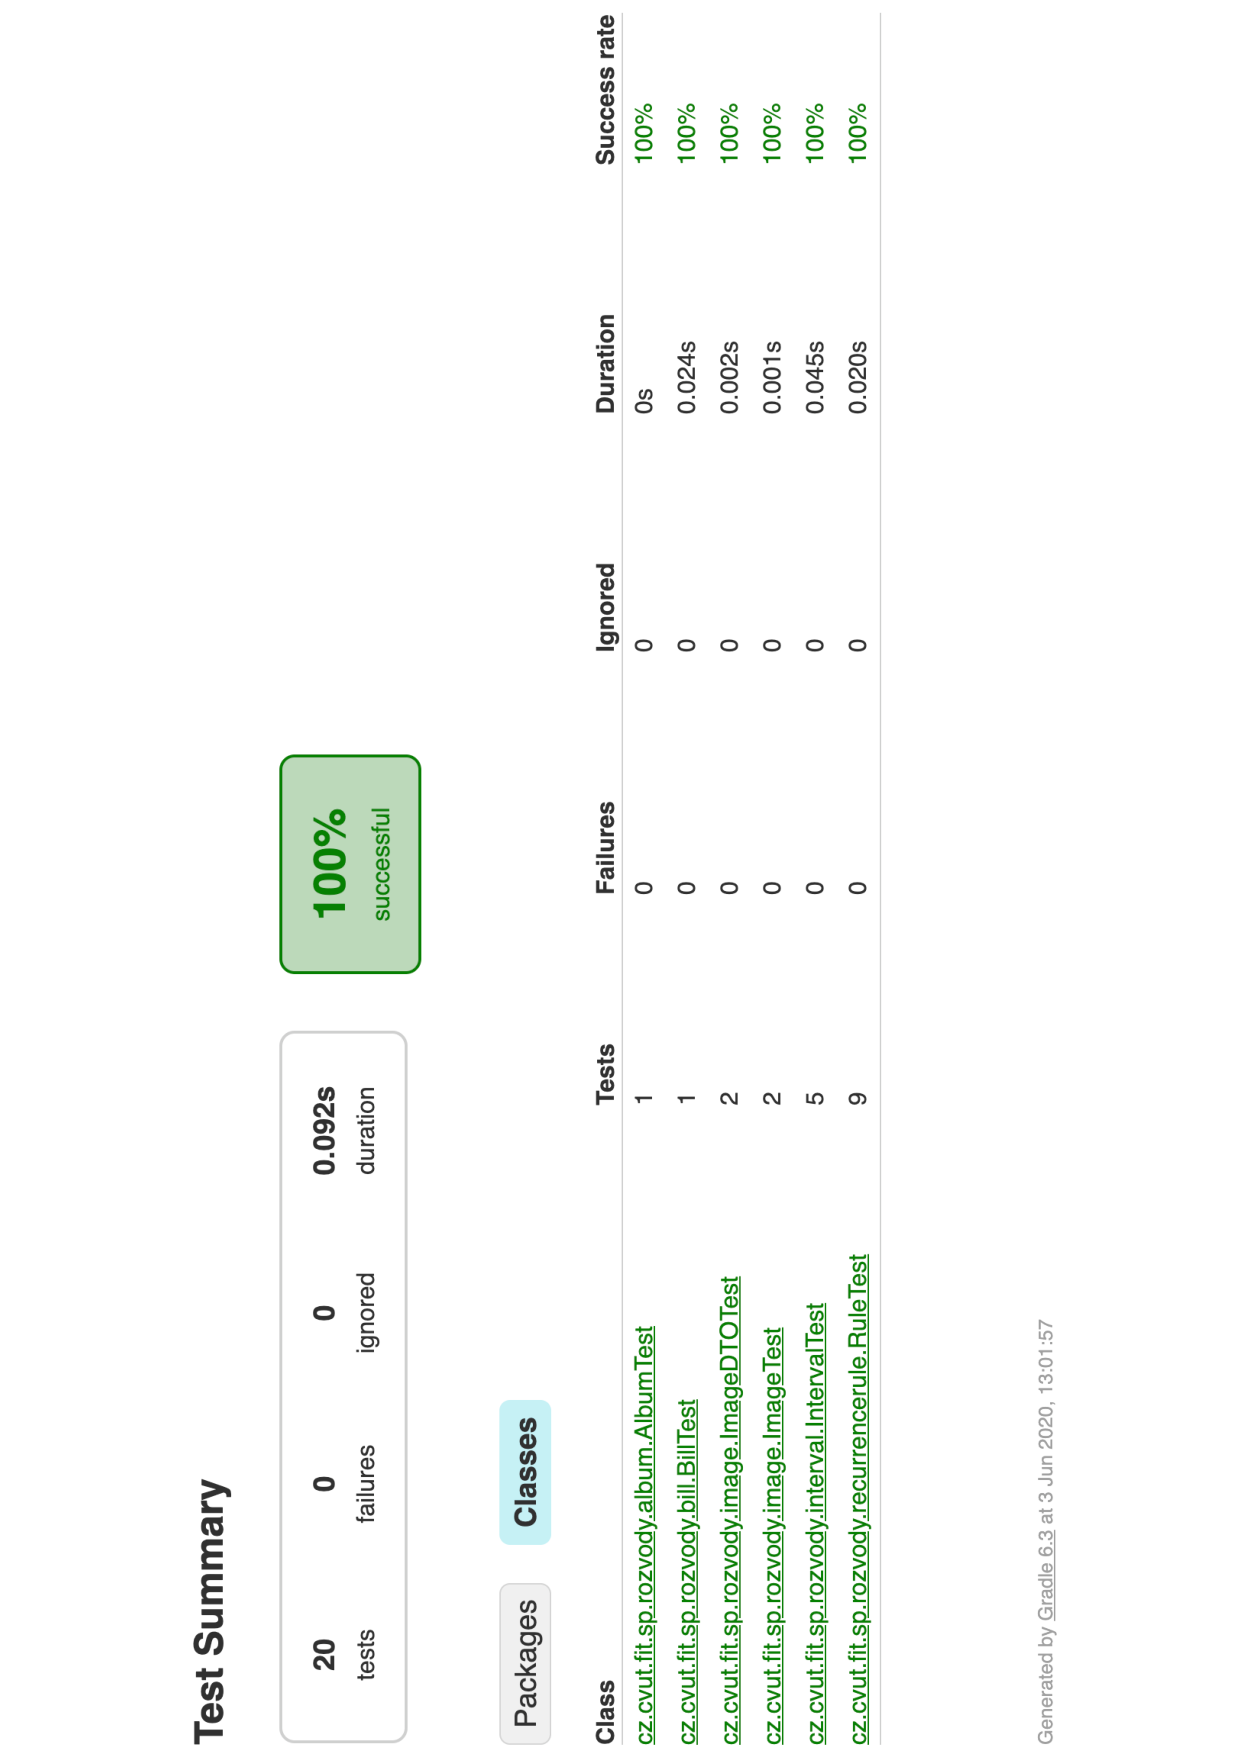
\includegraphics[width=1.0\textwidth]{pdfs/Gradle-integration-tests}
	    \caption[Seznam tříd obsahujících integrační testy]{Seznam tříd obsahující integračních testy vygenerovaný pomocí nástroje Gradle}\label{image:gradle-integration-tests}
    \end{figure}
    \begin{figure}\centering
	    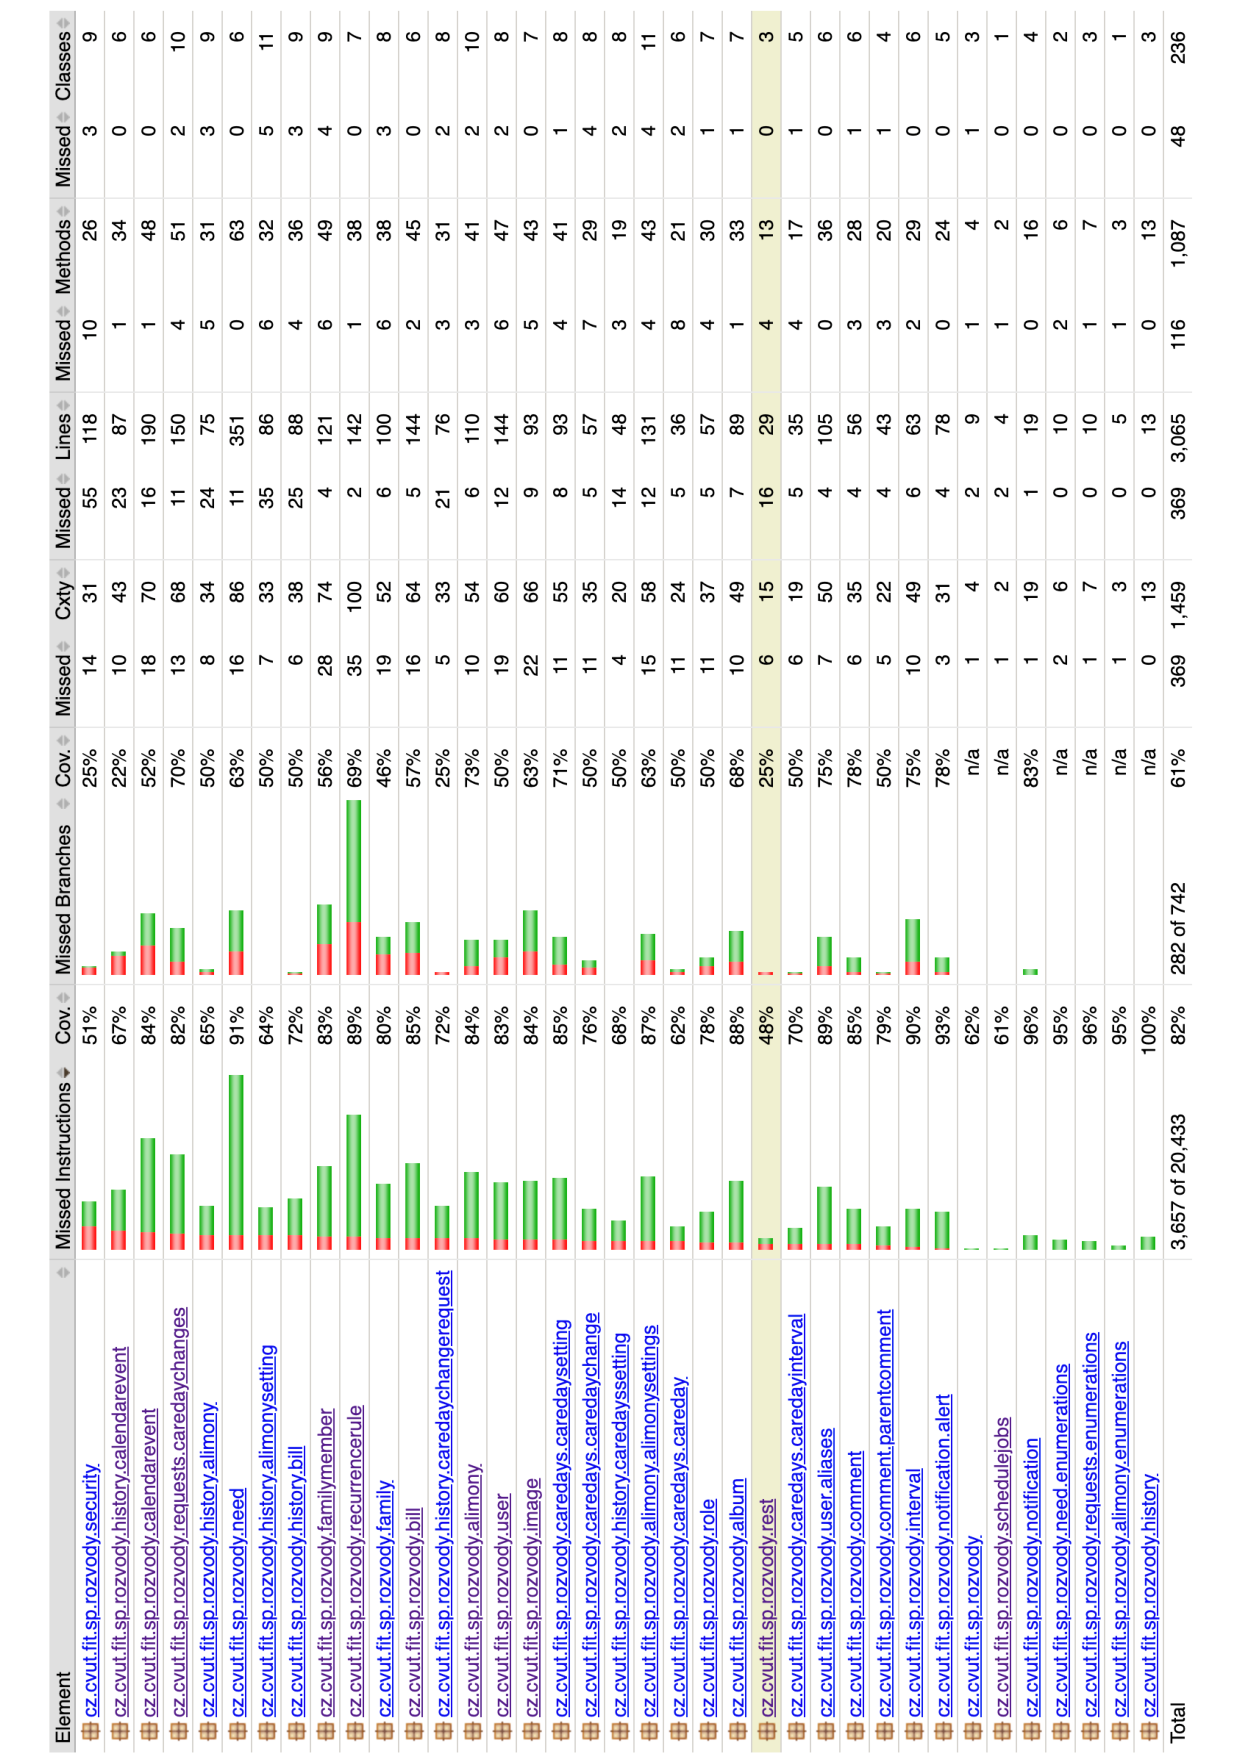
\includegraphics[width=1.0\textwidth]{pdfs/JaCoCo-results}
	    \caption[Pokrytí kódů testy podle JaCoCo]{Poslední verze výsledku pokrytí kódů testy podle JaCoCo}\label{image:jacoco-results}
    \end{figure}
    \begin{figure}\centering
	    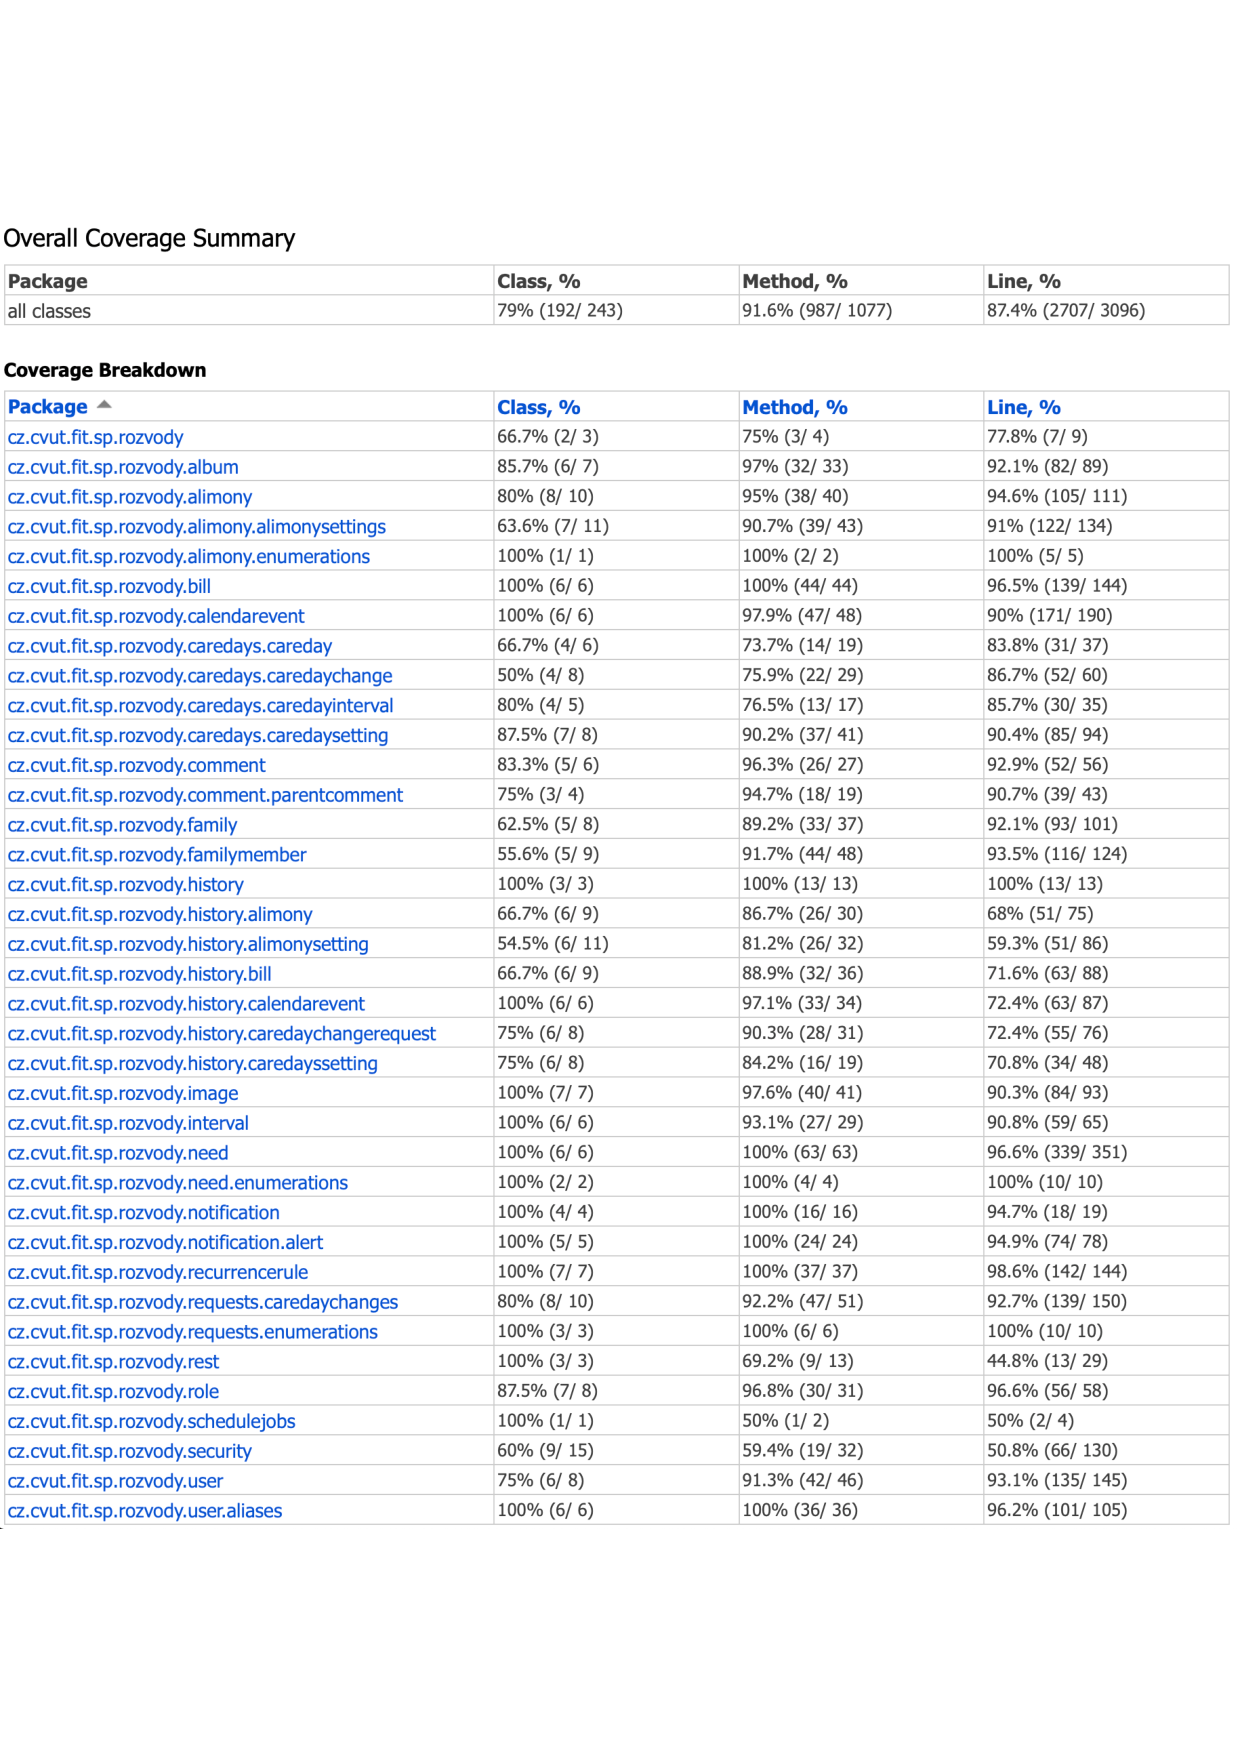
\includegraphics[width=1.0\textwidth]{pdfs/IntelliJ-IDEA-coverage-runner-results}
	    \caption[Pokrytí kódů testy podle JaCoCo]{Poslední verze výsledku pokrytí kódů testy podle IntelliJ IDEA}\label{image:intellij-coverage-result}
    \end{figure}
% TODO tady by měl být výsledný Domenový model
\chapter{Výsledný doménový model}\label{dodatek:DomainModel2}
    \begin{figure}\centering
	    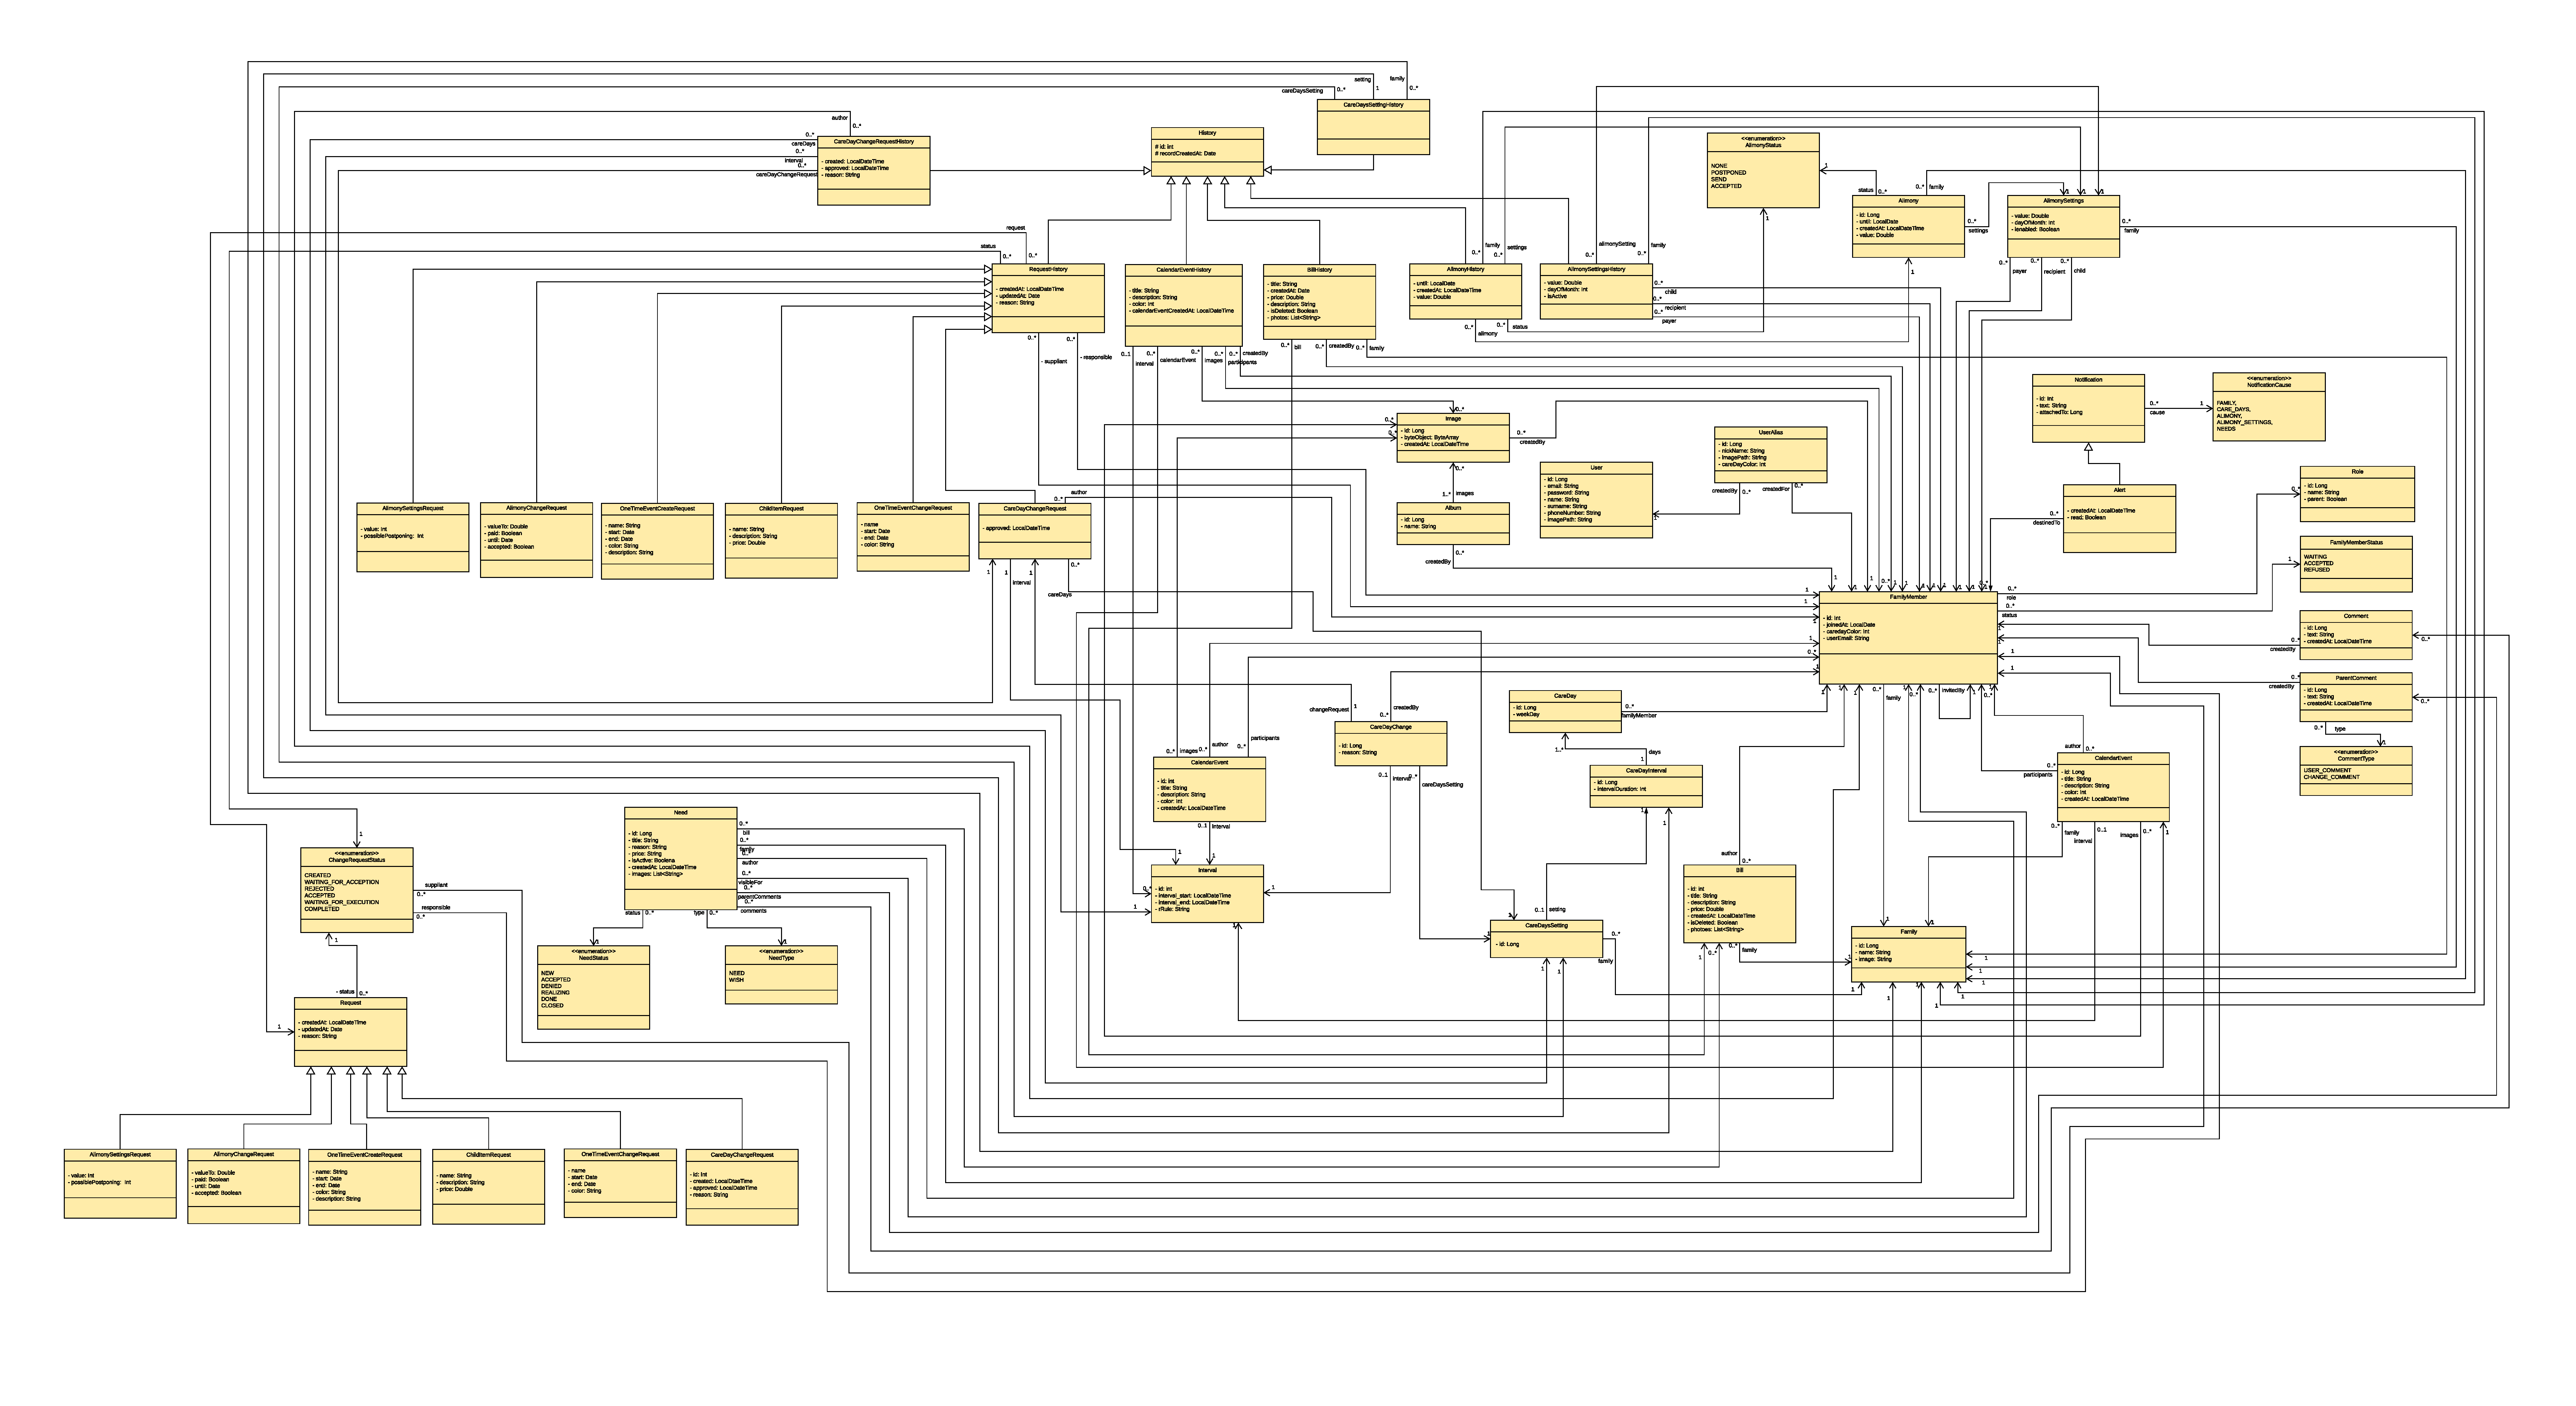
\includegraphics[angle=90, height=0.9\textheight]{pdfs/DomainModel2}
	    \caption[Výsledný doménový model]{Doménový model po navržení a implementaci všech úprav}\label{image:DomainModel2}
    \end{figure}
\chapter{Konfigurace výsledného našeptávače pro chyby}\label{dodatek:excpetion-handler2}
    % \begin{sidewaystable} \centering
    \begin{figure} \centering

    \begin{adjustbox}{angle=90} \centering
            \begin{tabular}{|l|c|c|c|}\hline
        	  Typ chyby		& HTTP status		& zpáva	& URL 	\tabularnewline \hline \hline
        	  \texttt{IllegalAccessException}	& 401	& původní zpráva chyby		& původní cesta     \tabularnewline \hline
        	  \texttt{IllegalArgumentException}	& 400	& původní zpráva chyby		& původní cesta     \tabularnewline \hline
        	  \texttt{NullPointerException}	& 500	& nic		& původní cesta     \tabularnewline \hline
        	  \texttt{No Such Element}	& 404	& nic		& nic     \tabularnewline \hline
        	  \texttt{MissingKotlinParameterException}	& 400	& původní zpráva chyby		& původní cesta     \tabularnewline \hline
            \end{tabular}
    % \end{sidewaystable}
    \end{adjustbox} \caption[Konfigurace výsledného našeptávače pro řadiče]{Ukázka výsledné konfigurace našeptávače zachycování výjimek pro řadiče}
    \end{figure}
\chapter{Obrázky}\label{dodatek:images}
    % ANALYZA
    \begin{figure}\centering
        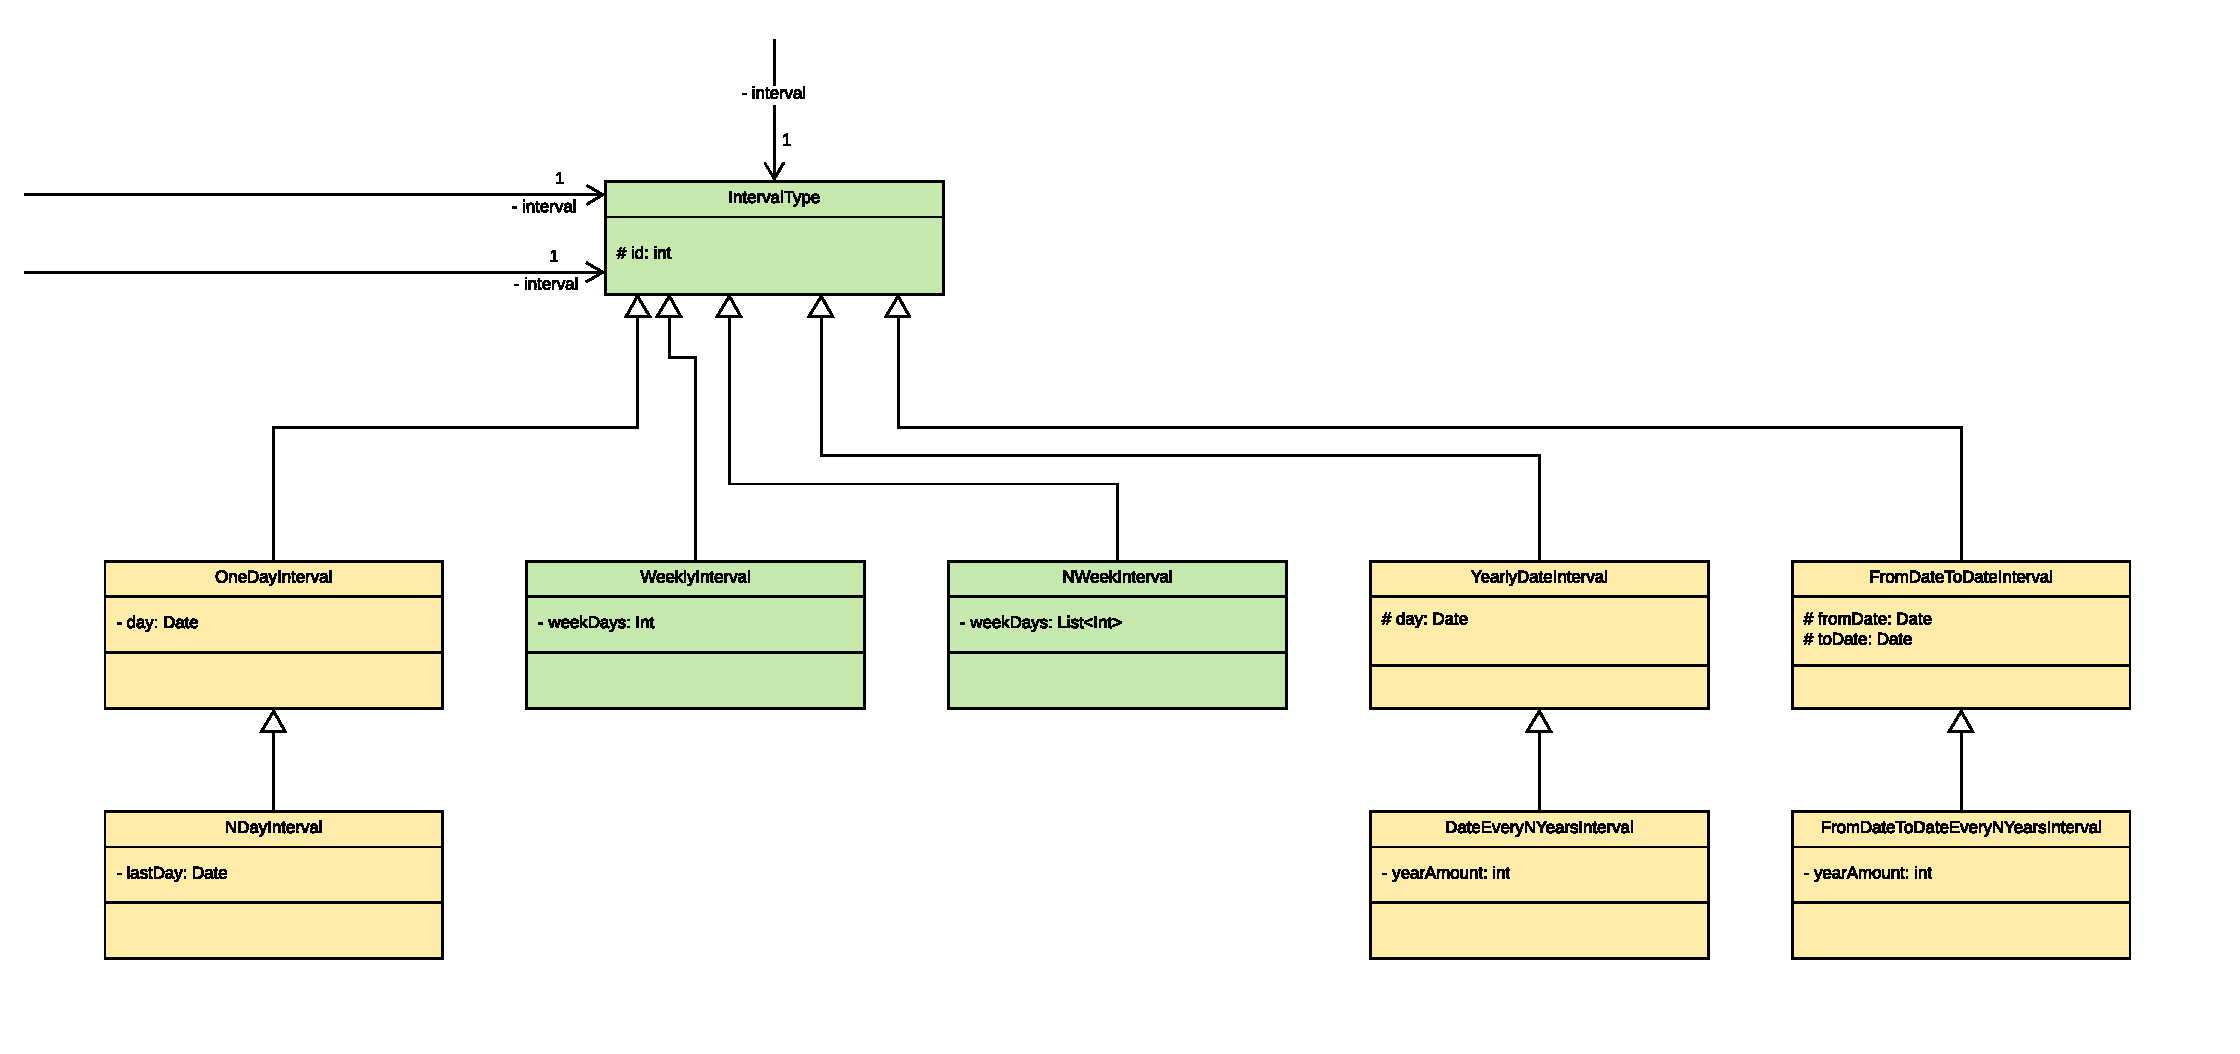
\includegraphics[angle=90, height=0.9\textheight]{pdfs/Interval1}
        \caption[Předešlý návrh entity \texttt{Interval}]{Návrh entity \textit{Interval} podle doménového modelu z předmětu BI-SP2}\label{image:Interval1}
    \end{figure}
    \begin{figure}\centering
            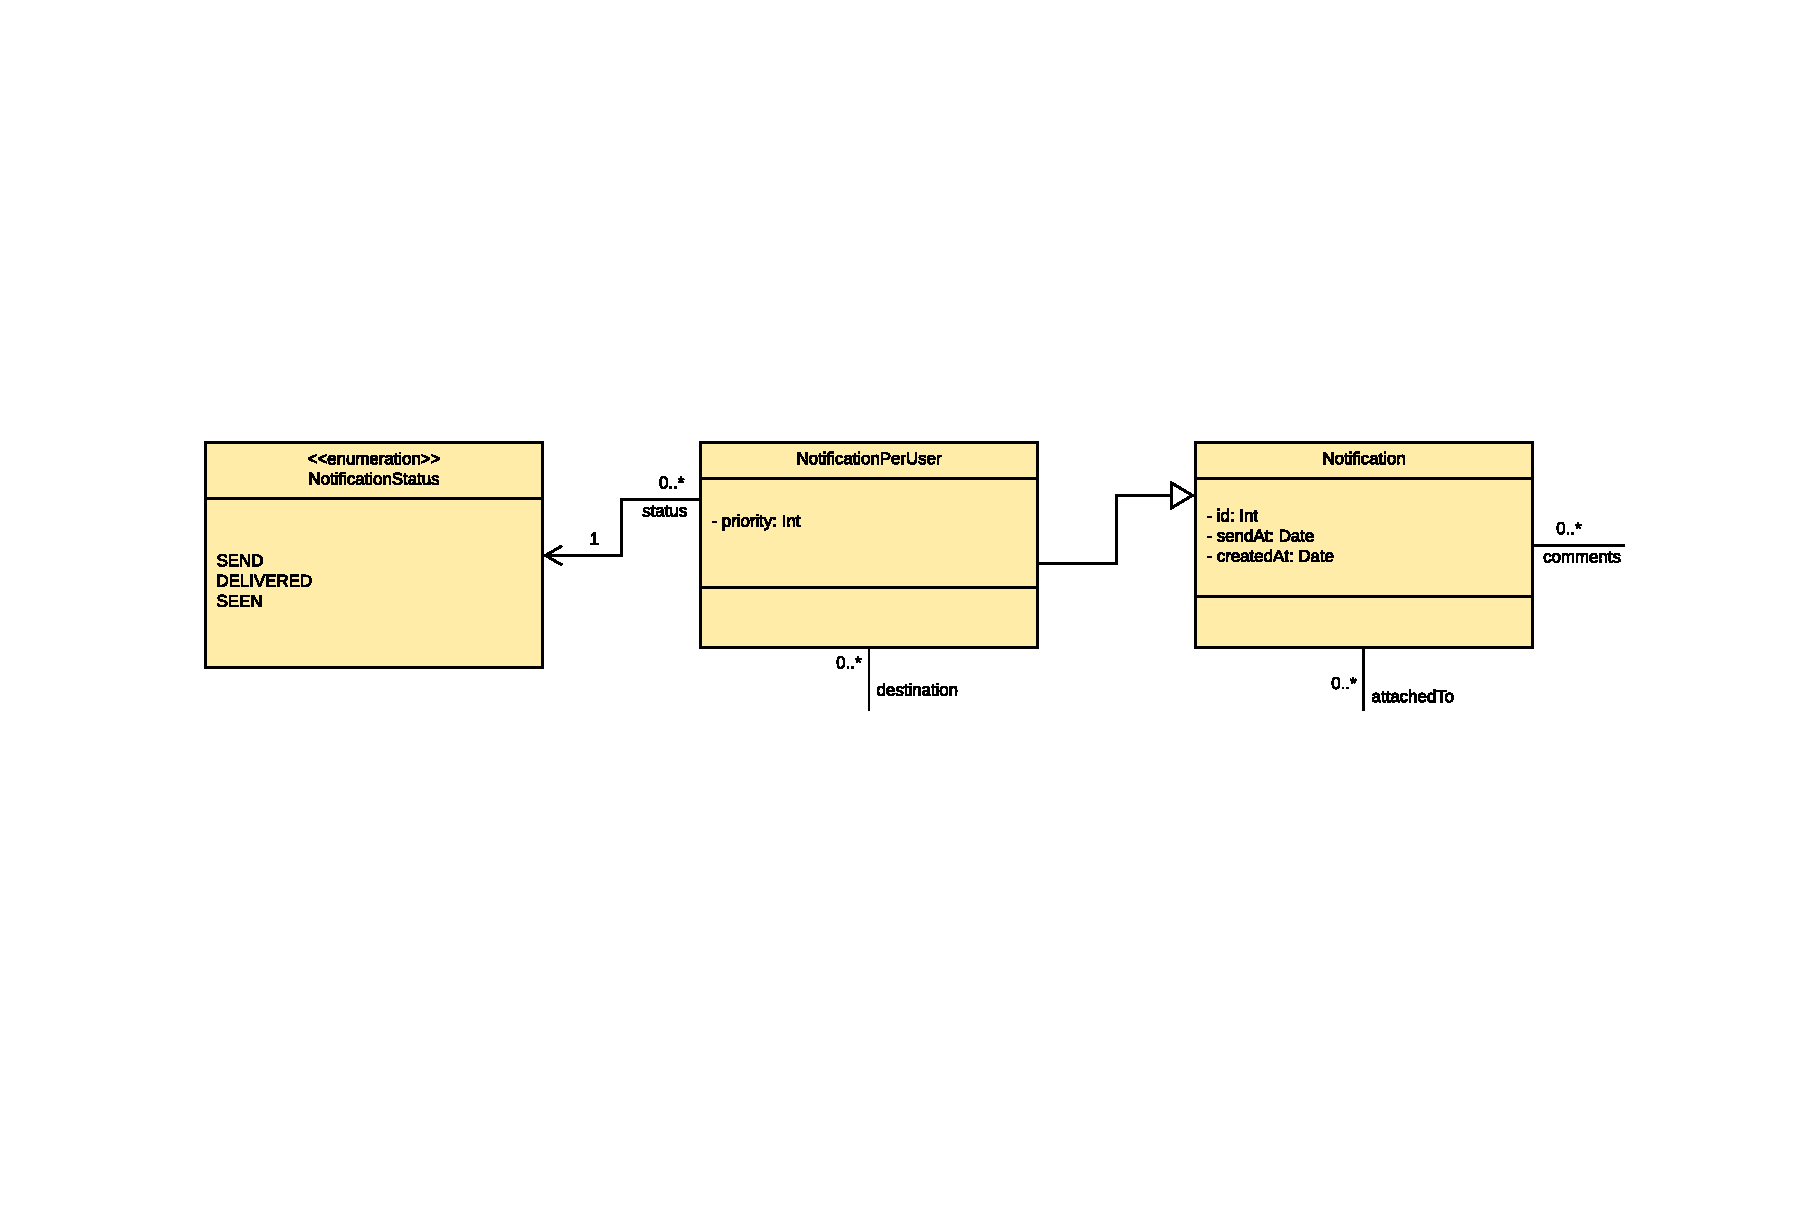
\includegraphics[angle=90, height=0.9\textheight]{pdfs/Notification1}
            \caption[Předešlý návrh oznámení]{Návrh oznámení podle doménového modelu předmětu BI-SP2}\label{image:notification1}
        \end{figure}
        \begin{figure}\centering
	        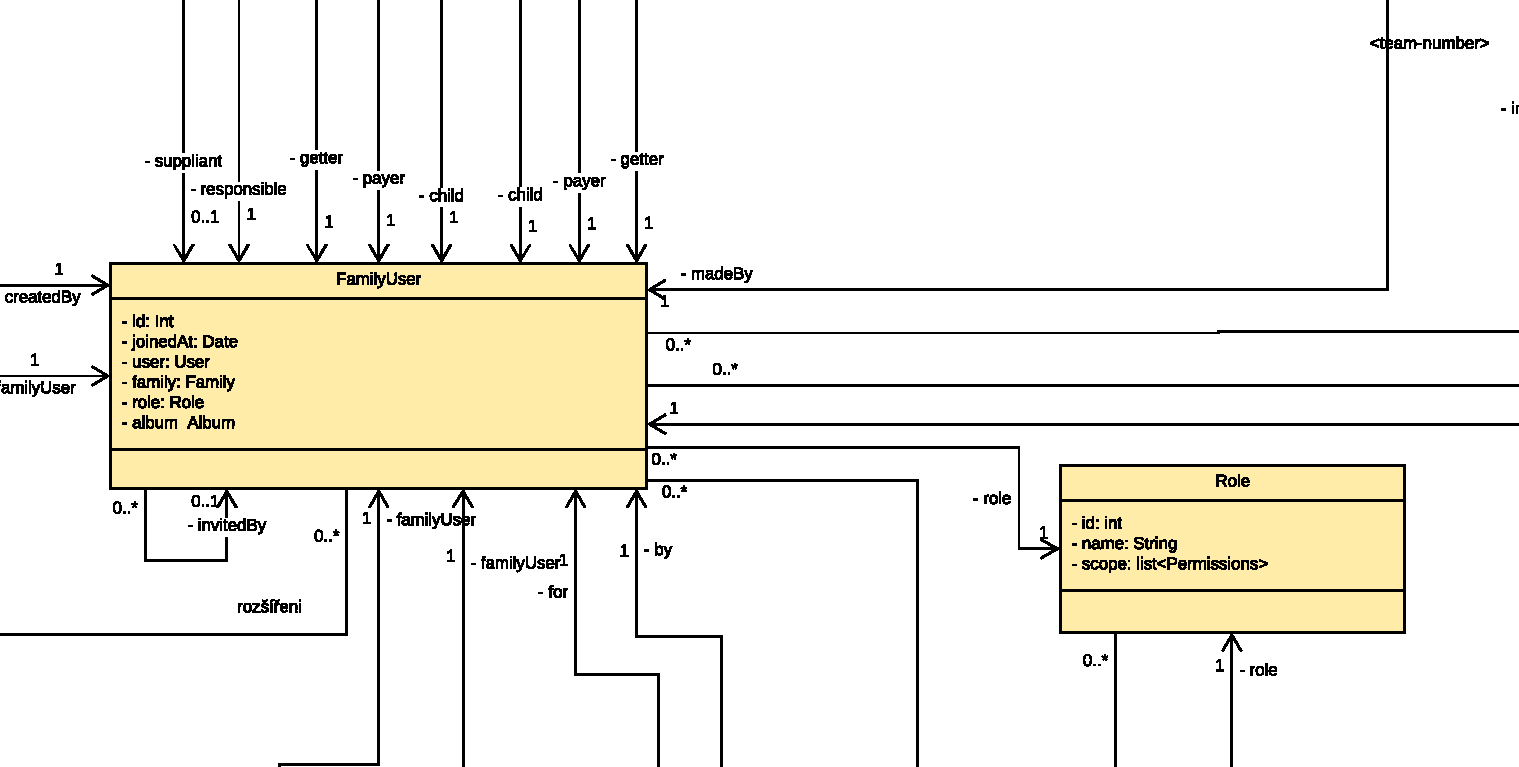
\includegraphics[angle=90, height=0.9\textheight]{pdfs/Role1}
	        \caption[Návrh \texttt{Role}]{Návrh entity \texttt{Role} podle doménového modelu z~předmětu BI-SP2}\label{image:Role1}
        \end{figure}
    % Navrh a Implementace 
    \begin{figure}\centering
	       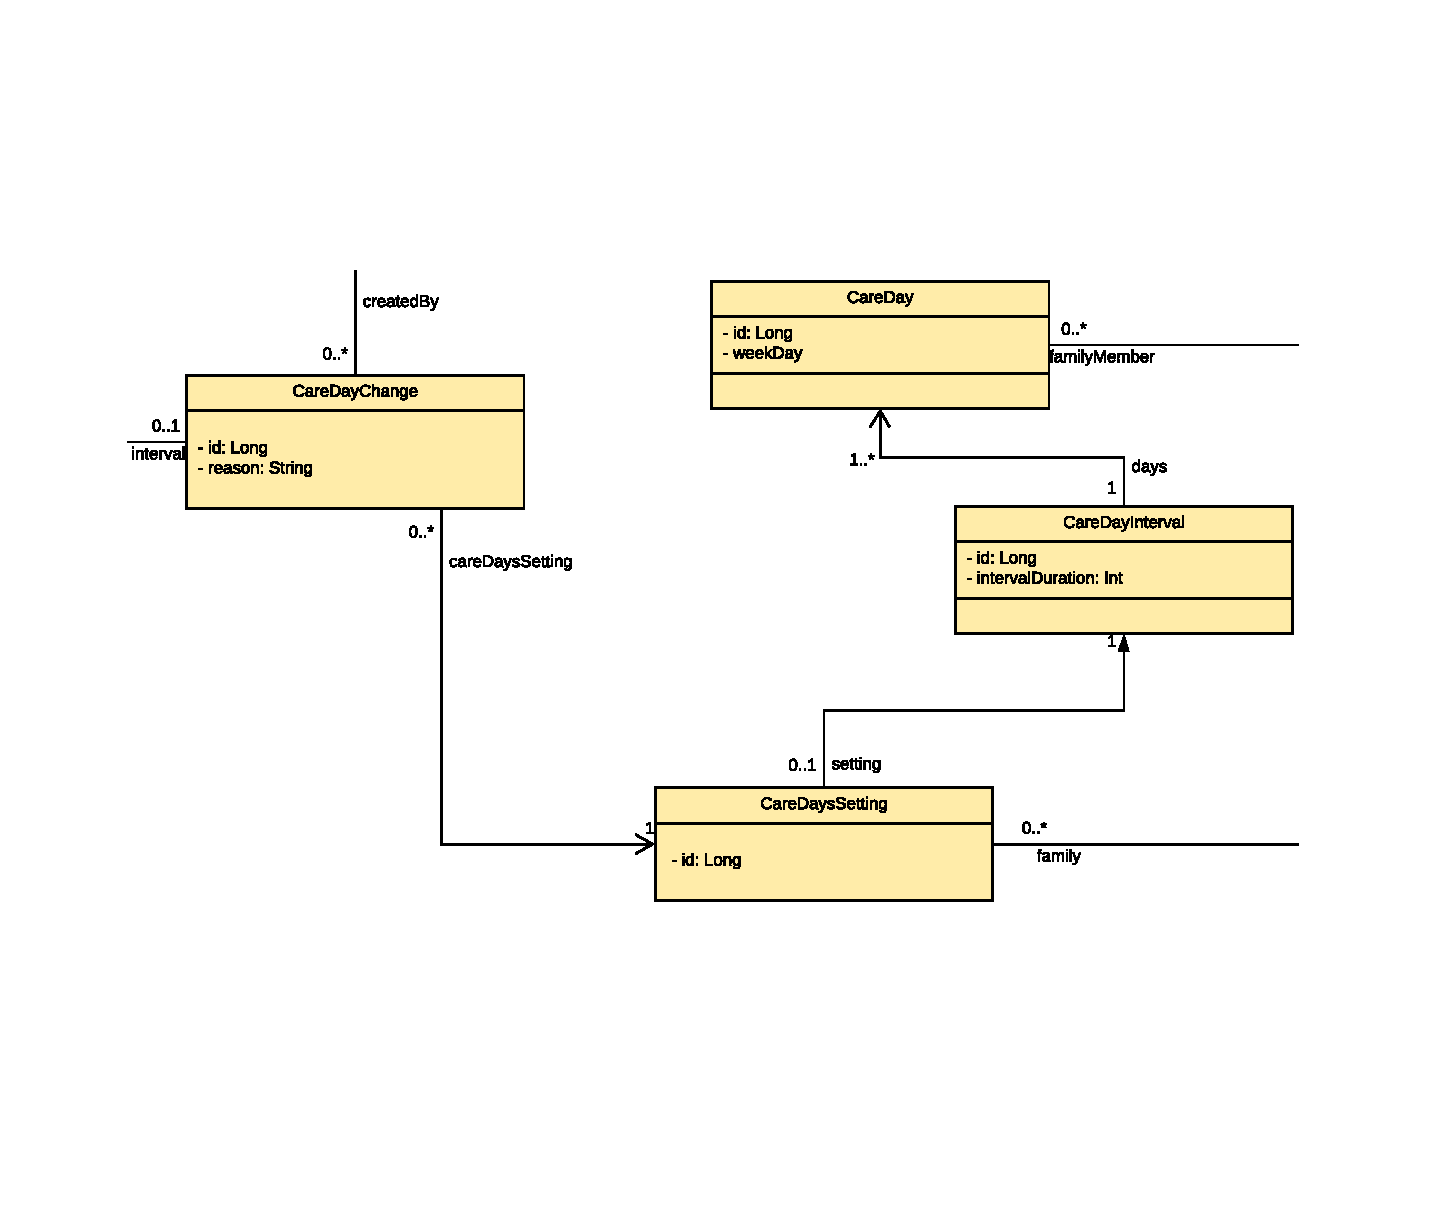
\includegraphics[angle=90, height=0.9\textheight]{pdfs/CareDays2}
	       \caption[Nový návrh pečovatelských dnů]{Nový návrh pečovatelských dnů}\label{image:caredays2}
        \end{figure}
          \begin{figure}\centering
	        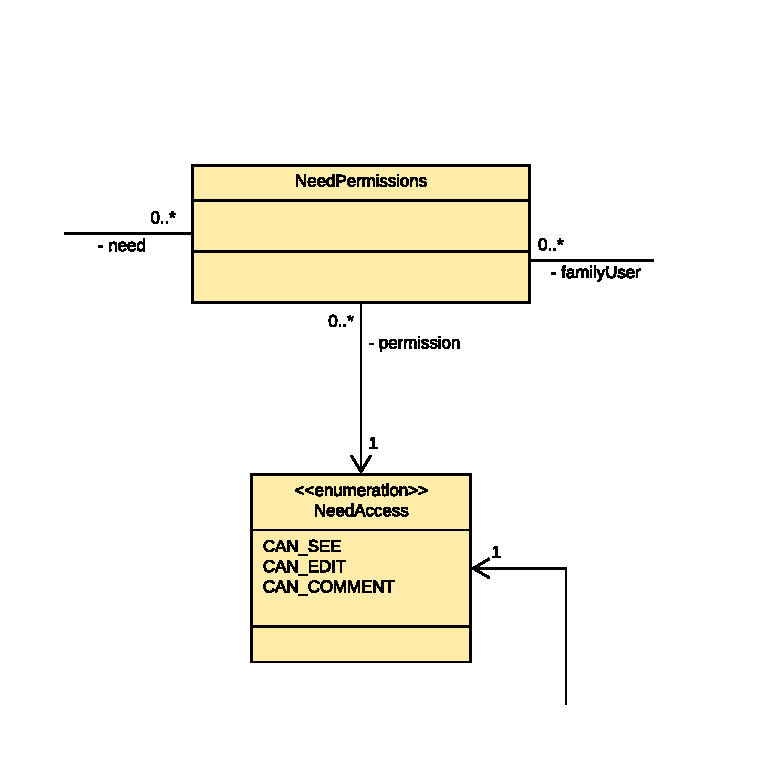
\includegraphics[width=1.0\textwidth]{pdfs/NeedPermissions1}
	        \caption[Návrh entity \texttt{NeedPermissions}]{Návrh entity \texttt{NeedPermissions} podle doménového modelu z~předmětu BI-SP2}\label{image:NeedPermissions1}
        \end{figure}
    \begin{figure}\centering
        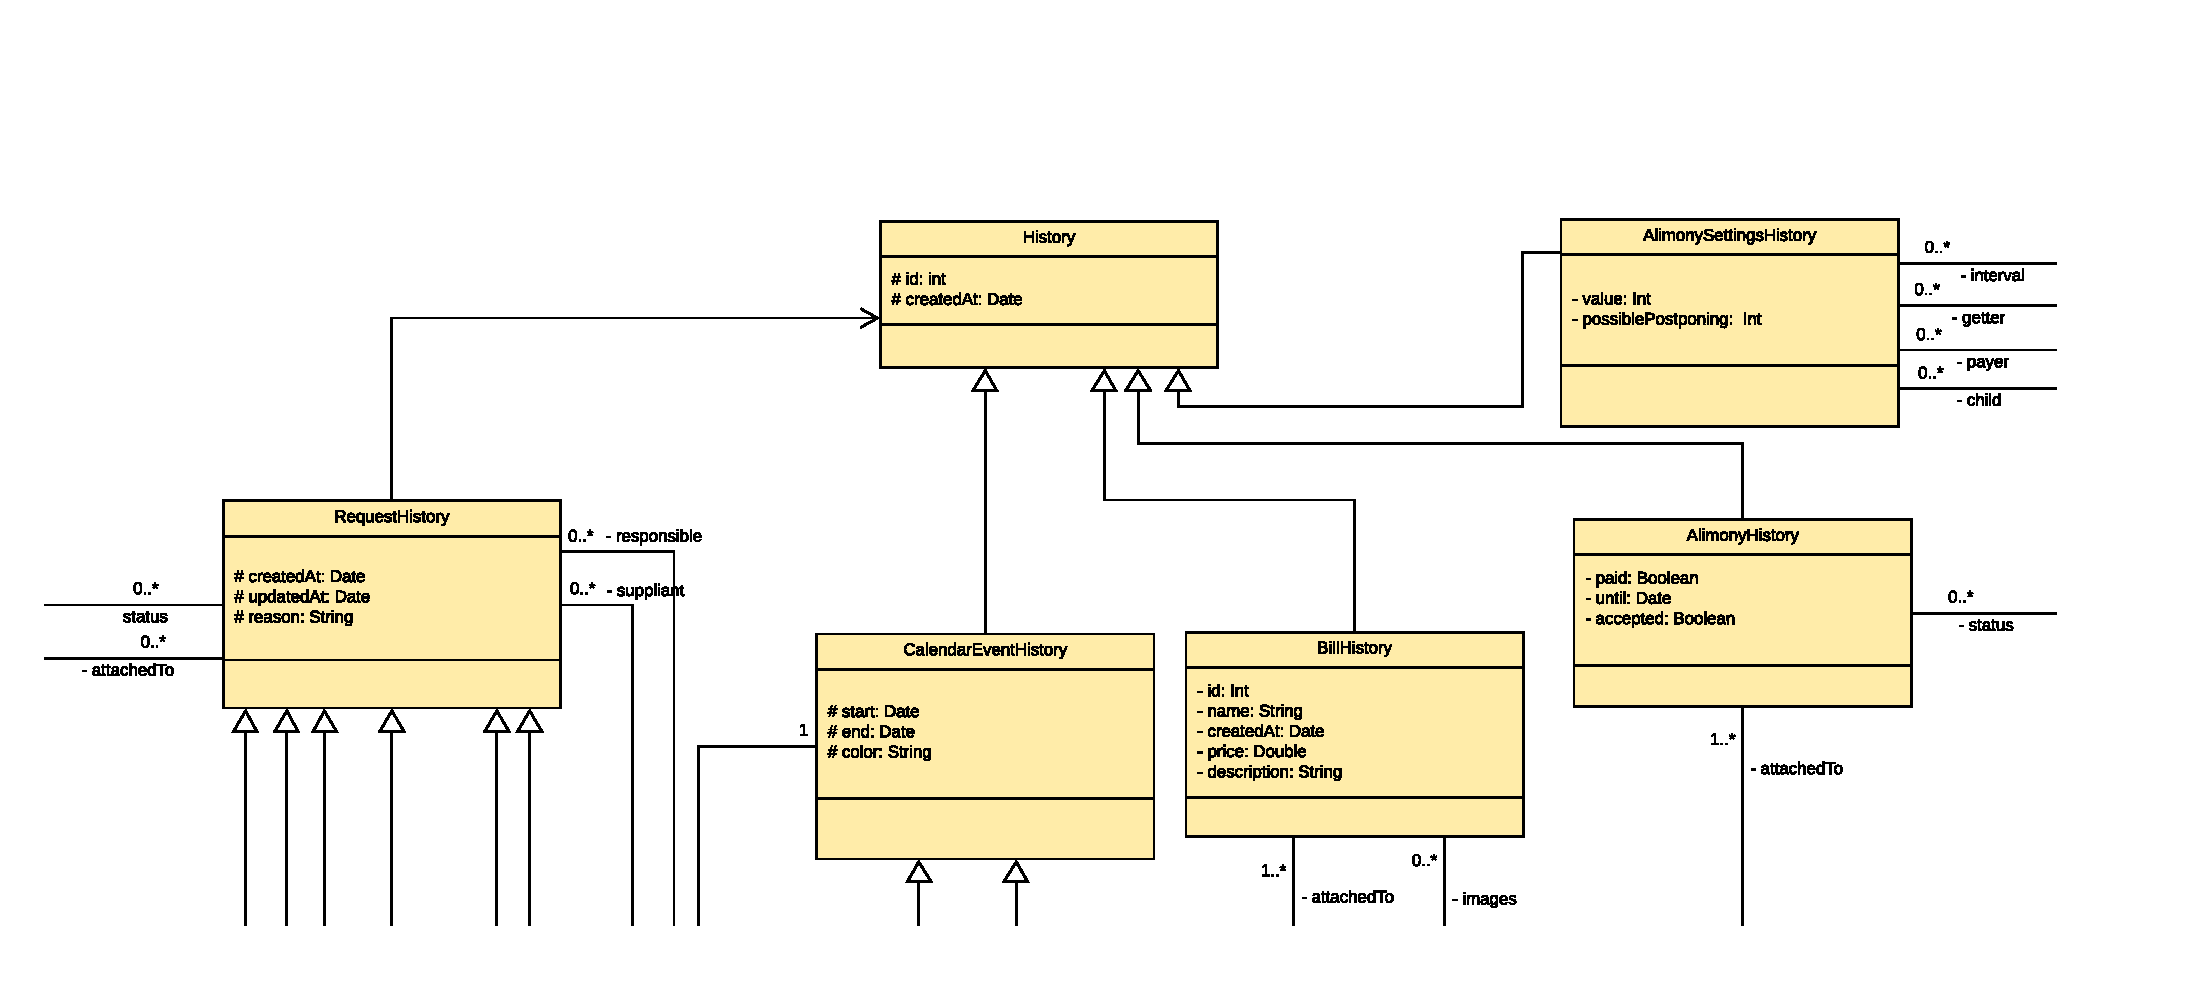
\includegraphics[angle=90, height=0.9\textheight]{pdfs/History1}
        \caption[Předešlý návrh entity \texttt{History}]{Předchozí návrh entity \texttt{History} podle doménového modelu z předmětu BI-SP2}\label{image:History1}
    \end{figure}
    \begin{figure}\centering
        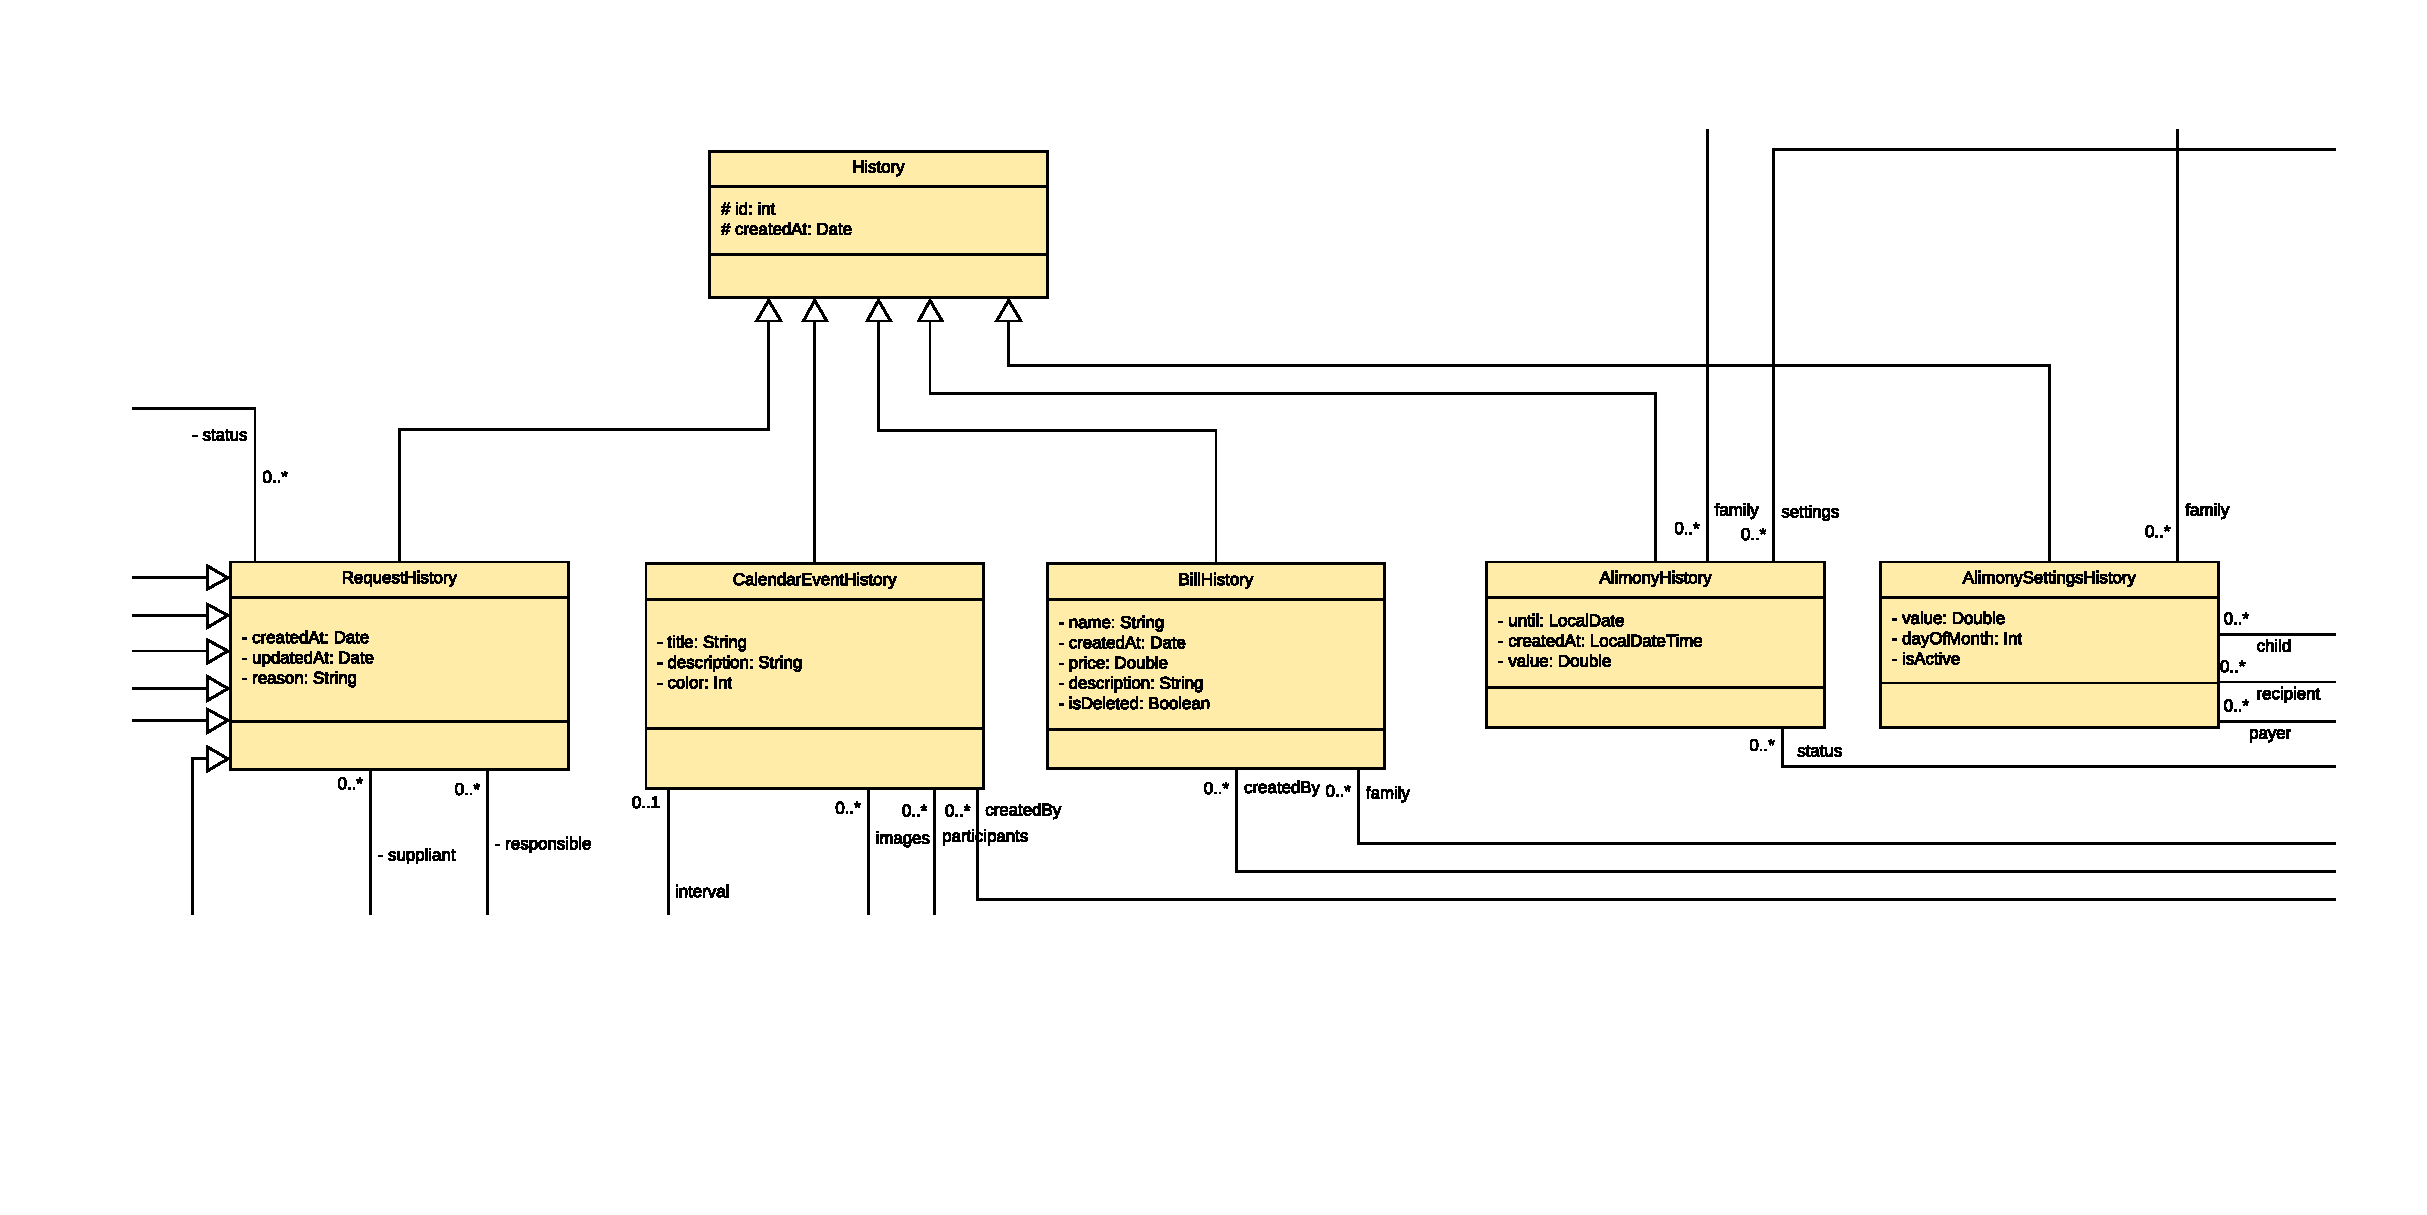
\includegraphics[angle=90, height=0.9\textheight]{pdfs/History1_2}
        \caption[Návrh entity \texttt{History} po změnách návrhu]{Návrh entity \texttt{History} po navržení změn pro entity, kterým patří příslušné entity historie}\label{image:History1_2}
    \end{figure}



%upravte podle skutecnosti

\chapter{Obsah přiloženého CD}

\begin{figure}
	\dirtree{%
		.1 README.md\DTcomment{stručný popis obsahu CD}.
		.1 jar\DTcomment{adresář se spustitelnou formou implementace}.
		.1 src.
		.2 impl\DTcomment{zdrojové kódy implementace}.
		.2 thesis\DTcomment{zdrojová forma práce ve formátu \LaTeX{}}.
		.1 text\DTcomment{text práce}.
		.2 thesis.pdf\DTcomment{text práce ve formátu PDF}.
		.2 thesis.ps\DTcomment{text práce ve formátu PS}.
	}
\end{figure}


\end{document}
